

\documentclass [
  english
% 	draft		% falls ohne Bilder gedruckt werden soll (Entwurf)
	]{scrbook}	% KOMA Klasse für Bücher

%%MOD%%
\usepackage{fhacmb}	% Style-File für Titelblatt. Ggf. bei Enning holen

\KOMAoptions{
	parskip=true,		% Absätze mit Abstand
	fontsize=12pt,		% Standardschriftgröße
	toc=flat,		% Inhaltsverzeichnis ohne Einzüge
	twoside=false,		% Einseitig setzen
	numbers=nodotatend,	% Nummerierungen nicht mit Punkt abschließen
% die folgenden Optionen nehmen die entsprechende Dinge ins Inhaltsverzeichnis auf
% mit der bei texlive vorhandenen aktuellen Version von pdflatex funkioniert es nicht mehr
% (bekannter Bug)
	toc=bibliography,	% Literaturverzeichnis ins Inhaltsverzeichnis
	toc=listof,		% Abbildung- und Tabellenverzeichnis ins Inhaltsverzeichnis
	toc=index,		% Stichwortverzeichnis ins Inhaltsverzeichnis
	}
%

\usepackage{amsmath,amssymb}






\IfFileExists{xcolor.sty}{
    \RequirePackage{xcolor}
}{
    \RequirePackage{color}
}


\providecommand{\tightlist}{%
  \setlength{\itemsep}{0pt}\setlength{\parskip}{0pt}}



\usepackage{footnotebackref}
\usepackage{graphicx}




%
% for the background color of the title page
%

%
% break urls
%
\PassOptionsToPackage{hyphens}{url}

%
% When using babel or polyglossia with biblatex, loading csquotes is recommended
% to ensure that quoted texts are typeset according to the rules of your main language.
%
\usepackage{csquotes}
%
% variables for title, author and date
%
\usepackage{titling}
%
% ADD SYNTAX HIGHLIGHTING
%

%
%
% Listings
%
%
\usepackage{listings}
\newcommand{\passthrough}[1]{#1}
\lstset{defaultdialect=[5.3]Lua}
\lstset{defaultdialect=[x86masm]Assembler}
%
% general listing colors
%
\definecolor{listing-background}{HTML}{F7F7F7}
\definecolor{listing-rule}{HTML}{B3B2B3}
\definecolor{listing-numbers}{HTML}{B3B2B3}
\definecolor{listing-text-color}{HTML}{000000}
\definecolor{listing-keyword}{HTML}{435489}
\definecolor{listing-keyword-2}{HTML}{1284CA} % additional keywords
\definecolor{listing-keyword-3}{HTML}{9137CB} % additional keywords
\definecolor{listing-identifier}{HTML}{435489}
\definecolor{listing-string}{HTML}{00999A}
\definecolor{listing-comment}{HTML}{8E8E8E}

\lstdefinestyle{eisvogel_listing_style}{
  language         = java,
  numbers          = left,
  xleftmargin      = 2.7em,
  framexleftmargin = 2.5em,
  backgroundcolor  = \color{listing-background},
  basicstyle       = \color{listing-text-color}\linespread{1.0}\small\ttfamily{},
  breaklines       = true,
  frame            = single,
  framesep         = 0.19em,
  rulecolor        = \color{listing-rule},
  frameround       = ffff,
  tabsize          = 4,
  numberstyle      = \color{listing-numbers},
  aboveskip        = 1.0em,
  belowskip        = 0.1em,
  abovecaptionskip = 0em,
  belowcaptionskip = 1.0em,
  keywordstyle     = {\color{listing-keyword}\bfseries},
  keywordstyle     = {[2]\color{listing-keyword-2}\bfseries},
  keywordstyle     = {[3]\color{listing-keyword-3}\bfseries\itshape},
  sensitive        = true,
  identifierstyle  = \color{listing-identifier},
  commentstyle     = \color{listing-comment},
  stringstyle      = \color{listing-string},
  showstringspaces = false,
  escapeinside     = {/*@}{@*/}, % Allow LaTeX inside these special comments
  literate         =
  {á}{{\'a}}1 {é}{{\'e}}1 {í}{{\'i}}1 {ó}{{\'o}}1 {ú}{{\'u}}1
  {Á}{{\'A}}1 {É}{{\'E}}1 {Í}{{\'I}}1 {Ó}{{\'O}}1 {Ú}{{\'U}}1
  {à}{{\`a}}1 {è}{{\'e}}1 {ì}{{\`i}}1 {ò}{{\`o}}1 {ù}{{\`u}}1
  {À}{{\`A}}1 {È}{{\'E}}1 {Ì}{{\`I}}1 {Ò}{{\`O}}1 {Ù}{{\`U}}1
  {ä}{{\"a}}1 {ë}{{\"e}}1 {ï}{{\"i}}1 {ö}{{\"o}}1 {ü}{{\"u}}1
  {Ä}{{\"A}}1 {Ë}{{\"E}}1 {Ï}{{\"I}}1 {Ö}{{\"O}}1 {Ü}{{\"U}}1
  {â}{{\^a}}1 {ê}{{\^e}}1 {î}{{\^i}}1 {ô}{{\^o}}1 {û}{{\^u}}1
  {Â}{{\^A}}1 {Ê}{{\^E}}1 {Î}{{\^I}}1 {Ô}{{\^O}}1 {Û}{{\^U}}1
  {œ}{{\oe}}1 {Œ}{{\OE}}1 {æ}{{\ae}}1 {Æ}{{\AE}}1 {ß}{{\ss}}1
  {ç}{{\c c}}1 {Ç}{{\c C}}1 {ø}{{\o}}1 {å}{{\r a}}1 {Å}{{\r A}}1
  {€}{{\EUR}}1 {£}{{\pounds}}1 {«}{{\guillemotleft}}1
  {»}{{\guillemotright}}1 {ñ}{{\~n}}1 {Ñ}{{\~N}}1 {¿}{{?`}}1
  {…}{{\ldots}}1 {≥}{{>=}}1 {≤}{{<=}}1 {„}{{\glqq}}1 {“}{{\grqq}}1
  {”}{{''}}1
}
\lstset{style=eisvogel_listing_style}

%
% Java (Java SE 12, 2019-06-22)
%
\lstdefinelanguage{Java}{
  morekeywords={
    % normal keywords (without data types)
    abstract,assert,break,case,catch,class,continue,default,
    do,else,enum,exports,extends,final,finally,for,if,implements,
    import,instanceof,interface,module,native,new,package,private,
    protected,public,requires,return,static,strictfp,super,switch,
    synchronized,this,throw,throws,transient,try,volatile,while,
    % var is an identifier
    var
  },
  morekeywords={[2] % data types
    % primitive data types
    boolean,byte,char,double,float,int,long,short,
    % String
    String,
    % primitive wrapper types
    Boolean,Byte,Character,Double,Float,Integer,Long,Short
    % number types
    Number,AtomicInteger,AtomicLong,BigDecimal,BigInteger,DoubleAccumulator,DoubleAdder,LongAccumulator,LongAdder,Short,
    % other
    Object,Void,void
  },
  morekeywords={[3] % literals
    % reserved words for literal values
    null,true,false,
  },
  sensitive,
  morecomment  = [l]//,
  morecomment  = [s]{/*}{*/},
  morecomment  = [s]{/**}{*/},
  morestring   = [b]",
  morestring   = [b]',
}

\lstdefinelanguage{C++}{
  morekeywords={
    % normal keywords (without data types)
    abstract,assert,break,case,catch,class,continue,default,
    do,else,enum,exports,extends,final,finally,for,if,implements,
    import,instanceof,interface,module,native,new,package,private,
    protected,public,requires,return,static,strictfp,super,switch,
    synchronized,this,throw,throws,transient,try,volatile,while,
    const,this,template,struct,union,volatile,auto,inline,noexcept,not_eq,
    const_cast,extern,namespace,mutable,reflexpr,reinterpret_cast,
    static_cast,throw,typedef,typeid,wchar_t,xor_eq,or_eq,asm,std
    % var is an identifier
    var
  },
  morekeywords={[2] % data types
    % primitive data types
    bool,char,int,float,double,void,wchar_t,string,short,signed,long,unsigned
  },
  morekeywords={[3] % literals
    % reserved words for literal values
    null,true,false,
  },
  sensitive,
  morecomment  = [l]//,
  morecomment  = [s]{/*}{*/},
  morecomment  = [s]{/**}{*/},
  morestring   = [b]",
  morestring   = [b]',
}

\lstdefinelanguage{QML}{
  morekeywords={
    % normal keywords (without data types)
    default,required,readonly,property,function,
    import,qsTr,delegate
  },
  morekeywords={[2] % data types
    % primitive data types
    QtQuick,TextInput,Text,Connections,Rectangle,Item,Button,MenuManager,
    Image,BusyIndicator,GraphChart,ListView,AnimatedImage,Flickable,TextEdit,
    BorderImage,FocusScope,MouseArea,CheckBox,CheckDelegate,ComboBox,DelayButton,Dial,
    Frame,GroupBox,ItemDelegate,Label,Page,PageIndicator,Pane,ProgressBar,
    RadioButton,RadioDelegate,RangeSlider,RoundButton,ScrollView,Slider,SpinBox,StackView,
    SwipeDelegate,SwipeView,Switch,SwitchDelegate,TabBar,TabButton,TextArea,TextField,ToolBar,
    ToolButton,ToolSeperator,Tumbler,ColumnLayout,GridLayout,RowLayout,StackLayout,
    Column,Flow,Grid,Row,GridView,ListView,PathView,
    ColorAnimation,NumberAnimation,ParallelAnimation,PauseAnimation,PropertyAction,PropertyAnimation,
    ScriptAction,SequentialAnimation
  },
  morekeywords={[3] % literals
    % reserved words for literal values
    null,true,false,id,x,y,width,height,color,visible,objectName,target,
    horizontalAlignment,wrapMode,change,value´
  },
  sensitive,
  morecomment  = [l]//,
  morecomment  = [s]{/*}{*/},
  morecomment  = [s]{/**}{*/},
  morestring   = [b]",
  morestring   = [b]',
}


\lstdefinelanguage{JavaScript}{
  keywords={typeof, new, true, false, catch, function, return, null, catch, switch, var, if, in, while, do, else, case, break},
  %keywordstyle=\color{blue}\bfseries,
  ndkeywords={class, export, boolean, throw, implements, import, this},
  %ndkeywordstyle=\color{darkgray}\bfseries,
  %identifierstyle=\color{black},
  sensitive=false,
  comment=[l]{//},
  morecomment=[s]{/*}{*/},
  %commentstyle=\color{purple}\ttfamily,
  %stringstyle=\color{red}\ttfamily,
  morestring=[b]',
  morestring=[b]"
}

\usepackage{xcolor}
\colorlet{punct}{red!60!black}
\definecolor{background}{HTML}{EEEEEE}
\definecolor{delim}{RGB}{20,105,176}
\colorlet{numb}{magenta!60!black}
\lstdefinelanguage{JSON}{
    basicstyle=\normalfont\ttfamily,
    numbers=left,
    %numberstyle=\scriptsize,
    %stepnumber=1,  
    %showstringspaces=false,
    breaklines=true,
    literate=
     *{0}{{{\color{numb}0}}}{1}
      {1}{{{\color{numb}1}}}{1}
      {2}{{{\color{numb}2}}}{1}
      {3}{{{\color{numb}3}}}{1}
      {4}{{{\color{numb}4}}}{1}
      {5}{{{\color{numb}5}}}{1}
      {6}{{{\color{numb}6}}}{1}
      {7}{{{\color{numb}7}}}{1}
      {8}{{{\color{numb}8}}}{1}
      {9}{{{\color{numb}9}}}{1}
      {:}{{{\color{punct}{:}}}}{1}
      {,}{{{\color{punct}{,}}}}{1}
      {\{}{{{\color{delim}{\{}}}}{1}
      {\}}{{{\color{delim}{\}}}}}{1}
      {[}{{{\color{delim}{[}}}}{1}
      {]}{{{\color{delim}{]}}}}{1},
}



\lstdefinelanguage{XML}{
  morestring      = [b]",
  moredelim       = [s][\bfseries\color{listing-keyword}]{<}{\ },
  moredelim       = [s][\bfseries\color{listing-keyword}]{</}{>},
  moredelim       = [l][\bfseries\color{listing-keyword}]{/>},
  moredelim       = [l][\bfseries\color{listing-keyword}]{>},
  morecomment     = [s]{<?}{?>},
  morecomment     = [s]{<!--}{-->},
  commentstyle    = \color{listing-comment},
  stringstyle     = \color{listing-string},
  identifierstyle = \color{listing-identifier}
}




%%%%%% Immer benötigte Packages
%
\usepackage[T1]{fontenc}		% sonst funktioniert die Silbentrennung bei Umlauten nicht
\usepackage[utf8]{inputenc}	% Eingabedekodierung. Ermöglicht Umlaute. Achtung: Unbedingt mit Betreuer
				% Verwendung der Umlaute-Eingabemethode absprechen. Im Zweifel \"O für Ö
\usepackage[ngerman]{babel}	% Silbentrennung und Sprachanpassung
\usepackage{blindtext}		% Blindtext

%\usepackage[hidelinks]{hyperref}		% Sprungmarken, z.B. im Inhaltsverzeichnis auf Textpassagen



\usepackage{graphicx}		% Definiert o.a. \includegraphics
\usepackage[export]{adjustbox}
\let\oldincludegraphics\includegraphics
\renewcommand{\includegraphics}[2][]{%
  \oldincludegraphics[#1,max width=\linewidth]{#2}}



\usepackage{textcomp}		% Sonst funktioniert z.B. \texteuro nicht
\usepackage{scrlayer-scrpage}	% Package zum Definieren der Kopf- und Fußzeilen
\usepackage{amsmath,amssymb}		% Muss sein
\usepackage{mathrsfs} 	% Weitere Mathematik-Symbole, z.B. Laplace-L
%
%%%%% Anpassung an Formatvorlagen des Fachbereichs
%
\usepackage{helvet}		% Serifenlose Schrift ähnlich Arial
\renewcommand{\familydefault}{\sfdefault}	% als Standardschrift serifenlose Schrift verwenden
%
\usepackage{geometry} 		% Ränder direkt einstellen
\geometry{a4paper, top=20mm, left=30mm, right=20mm, bottom=25mm} % nach Vorgabe
\linespread{1.25} 		% Zeilenabstand nach Vorgabe
%
\usepackage{chngcntr}		% Ändert Verhalten von Countern
\counterwithout{figure}{section}	% Figure-Nummerierung nicht bei section-Wechsel zurücksetzen
\renewcommand{\thefigure}{\textbf\thechapter-\arabic{figure}}	% im Stil 3-2
%
%%%% für das Erzeugen von Grafiken mit Zeichenbefehlen
%
\usepackage{tikz}		% Grundpaket
\usetikzlibrary{shapes,arrows}	% einige Symbolpackages
\usepackage{tikz-cd}		% einige Symbolpackages

%
%%%% TABELLEN
%
\usepackage{colortbl}		% für die Hintergrundfarbe von Tabellen
\usepackage{paralist}		% Weitere Nummeriungsoptionen, z.b. alphabetisch für enumerate/itemize

\usepackage{longtable}% FOR PANDOC TABLE GENERATOR
\usepackage{booktabs} % FOR TOPRULE MIDRULE

%
%%%% CODE
%
\usepackage{listings}

\lstset{ 
%  backgroundcolor=\color{white},   % choose the background color; you must add \usepackage{color} or \usepackage{xcolor}; should come as last argument
  basicstyle=\footnotesize,        % the size of the fonts that are used for the code
  breakatwhitespace=false,         % sets if automatic breaks should only happen at whitespace
  breaklines=true,                 % sets automatic line breaking
  captionpos=b,                    % sets the caption-position to bottom
  extendedchars=true,              % lets you use non-ASCII characters; for 8-bits encodings only, does not work with UTF-8
 % frame=single,	                   % adds a frame around the code
  keepspaces=true,                 % keeps spaces in text, useful for keeping indentation of code (possibly needs columns=flexible)
%  keywordstyle=\color{blue},       % keyword style
  numbers=left,                    % where to put the line-numbers; possible values are (none, left, right)
  numbersep=5pt,                   % how far the line-numbers are from the code
%  rulecolor=\color{black},         % if not set, the frame-color may be changed on line-breaks within not-black text (e.g. comments (green here))
  tabsize=2,	                   % sets default tabsize to 2 spaces
  title=\lstname                   % show the filename of files included with \lstinputlisting; also try caption instead of title
}

%
%%%% UNORDERED LISTS
%
\renewcommand{\labelitemii}{$\circ$} % Bullets für itemize-Listen



%
%%%% PAGE AND FIGURE NUMBERING
%
\usepackage{chngcntr}		% Ändert Verhalten von Countern
\counterwithout{figure}{section}	% Figure-Nummerierung nicht bei section-Wechsel zurücksetzen
\renewcommand{\thefigure}{\textbf\thechapter-\arabic{figure}}	% im Stil 3-2

%\usepackage{subfig}		% Unterfigures mit eigenen Bildunterschriften
\usepackage{caption}
\captionsetup[table]{name=Table}
%\setcounter{tocdepth}{3} % SHOW SUB SUB SUB SUB SECTIONS


%
%%%% acronyms
%



\usepackage{pdflscape}

%\usepackage{hyperref}
%\usepackage[colorlinks=true, urlcolor=blue, linkcolor=red]{hyperref}


\usepackage[acronym]{glossaries}
\makeglossaries

\makeglossaries
\newacronym{ic}{IC}{Integrated Circuit}
\newacronym{mrp}{MRP}{MagneticReadoutProcessing}
\newacronym{mri}{MRI}{Magnetic Resonance Imaging}
\newacronym{rest}{REST}{Representational State Transfer}
\newacronym{pc}{PC}{Personal Computer}
\newacronym{ip}{IP}{Internet Protocol}
\newacronym{usb}{USB}{Universal Serial Bus}
\newacronym{ptp}{PTP}{Precision Time Protocol}
\newacronym{pps}{PPS}{Puls Per Second}
\newacronym{i2c}{I2C}{Inter-Integrated Circuit}
\newacronym{cli}{CLI}{Command Line Interface}
\newacronym{pip}{PIP}{Python Package Installer}
\newacronym{hal}{HAL}{Hardware Abstraction Layer}
\newacronym{pdf}{PDF}{Portable Document Format}
\newacronym{html}{HTML}{Hypertext Markup Language}
\newacronym{ide}{IDE}{Integrated Development Environment}
\newacronym{gui}{GUI}{Graphical User Interface}
\newacronym{sbc}{SBC}{Single Board Computer}
\newacronym{gpio}{GPIO}{General Purpose Input/Output}
\newacronym{uart}{UART}{Universal Asynchronous Receiver / Transmitter}
\newacronym{lut}{LUT}{Lookup Table}
\newacronym{cdc}{CDC}{Communication Device Class}
\newacronym{cad}{CAD}{Computer Aided Design}
\newacronym{json}{JSON}{JavaScript Object Notation}
\newacronym{id}{ID}{Identification Number}
\newacronym{pcb}{PCB}{Printed Circuit Board}
\newacronym{os}{OS}{Operating System}
\newacronym{uuid}{UUID}{Universal Unique Identifier}
\newacronym{nmr}{NMR}{Nuclear Magnetic Resonance}
\newacronym{dut}{DUT}{Device Under Test}
\newacronym{ppm}{ppm}{Parts Per Million}
\newacronym{snr}{SNR}{Signal to Noise Ratio}
\newacronym{sd}{SD}{Standard Deviation}
\newacronym{yaml}{YAML}{Yet Another Markup Language}
\newacronym{dr}{DR}{Dynamic Range}
\newacronym{mds}{MDS}{Minimum Detectable Signal}
\newacronym{cog}{CoG}{Center Of Gravity}
\newacronym{adc}{ADC}{Analog to Digital Converter}
\newacronym{ai}{AI}{Artificial Intelligence}
\newacronym{pla}{PLA}{Polylactic Acid}





%
%%%%%%%%%%  Angaben für Titelseite %%%%%%%%%%%%%%%%%%%%%%
%
% Angaben für Titelseite
\arbeitstyp{Masterarbeit}
\fachbereich{Fachbereich 5}
\studiengang{Information Systems Engineering}
\vertiefung{Systeme und Management}
\titel{Information Systems Engineering}
\autor{Marcel Werner Heinrich Friedrich Ochsendorf}
\matrnr{3120232}
\betreuer{Prof. Dr.-Ing. Thomas Dey}
\cobetreuer{Prof. Dr.-Ing. Volkmar Schulz}
%\extbetreuer{- extbetreuer -}
\datum{08.01.2024}
%\dank{- dank -}





%\hypersetup{draft} %DISBALE HYPERLINKS
% https://charly-lersteau.com/posts/2019-12-26-latex-hyperref-error-pdfendlink/
%\usepackage{etoolbox}

%\makeatletter
%\patchcmd\@combinedblfloats{\box\@outputbox}{\unvbox\@outputbox}{}{%
 %   \errmessage{\noexpand\@combinedblfloats could not be patched}%
%}%
%\makeatother

\usepackage{rotating}

\definecolor{LightCyan}{rgb}{0.88,1,1}
\definecolor{Gray}{gray}{0.9}
\usepackage[first=0,last=9]{lcg}
\newcommand{\ra}{\rand0.\arabic{rand}}


% ADD PAGE PACING FOR BETTER READABLE TABLES
\newcolumntype{g}{>{\columncolor{Gray}}c}
\renewcommand*{\arraystretch}{2} %2.0 IS  THE SPACING

\begin{document}



%%MOD%%
% Einige Anpassungen müssen nach \begin{document} stehen !!
\renewcaptionname{ngerman}{\figurename}{\textbf Figure} 	% Bild ... statt Abbildung ...
\renewcaptionname{ngerman}{\contentsname}{Contents}% Inhalt statt Inhaltsverzeichnis
\renewcaptionname{ngerman}{\bibname}{Bibliography}
\renewcaptionname{ngerman}{\tablename}{Table}
\renewcaptionname{ngerman}{\listfigurename}{List of Figures}
\renewcaptionname{ngerman}{\listtablename}{List of Tables}

\renewcommand*{\acronymname}{List of abbreviations}
% printglossaries
%%%%%%%%%%%%%%%%%%%%%%%%%%%%%%%%%%%%%%%%%%%%%%%%%%%%%%%%%%%%
% Titel im FH Style
%%%%%%%%%%%%%%%%%%%%%%%%%%%%%%%%%%%%%%%%%%%%%%%%%%%%%%%%%%%%
\fhacmbtitle{
\includegraphics[height=4cm]{fh_logo}}{5pt}{5pt}
%%%%%%%%%%%%%%%%%%%%%%%%%%%%%%%%%%%%%%%%%%%%%%%%%%%%%%%%%%%%
% Erklärung / Geheimhaltung
%%%%%%%%%%%%%%%%%%%%%%%%%%%%%%%%%%%%%%%%%%%%%%%%%%%%%%%%%%%%
%\frontmatter 	% Wenn der Hauptteil mit Seite 1 beginnen soll
\pagestyle{plain}








\frontmatter

%%%%%%%%%%%%%%%%%%%%%%%%%%%%%%%%%%%%%%%%%%%%%%%%%%%%%%%%%%%%
% Erklaerung
%%%%%%%%%%%%%%%%%%%%%%%%%%%%%%%%%%%%%%%%%%%%%%%%%%%%%%%%%%%%
\newpage

\hypertarget{erkluxe4rung}{%
\section*{Erklärung}\label{erkluxe4rung}}
Hiermit erkläre ich, dass ich die vorliegende Arbeit eigenständig und
ohne fremde Hilfe angefertigt habe. Textpassagen, die wörtlich oder dem
Sinn nach auf Publikationen oder Vorträgen anderer Autoren beruhen, sind
als solche kenntlich gemacht. Die Arbeit wurde bisher keiner anderen
Prüfungsbehörde vorgelegt und auch noch nicht veröffentlicht.

Aachen, den \datum  \_\_\_\_\_\_\_\_\_\_\_\_,
\_\_\_\_\_\_\_\_\_\_\_\_\_\_\_\_\_\_\_\_\_\_\_\_



%%%%%%%%%%%%%%%%%%%%%%%%%%%%%%%%%%%%%%%%%%%%%%%%%%%%%%%%%%%%
% ABSTRACT
%%%%%%%%%%%%%%%%%%%%%%%%%%%%%%%%%%%%%%%%%%%%%%%%%%%%%%%%%%%%
\newpage

\hypertarget{abstract}{%
\section*{Abstract}\label{abstract}}
In the construction of low-field MRI devices based on permanent magnets,
a large number of magnets are used. In order to realize a homogeneous B0
field with these magnets, which is necessary for many setups, the
magnetic properties of these magnets have to be as similar to a certain
degree. Due to the complex manufacturing process of neodymium magnets,
the different properties, the direction of magnetization, can deviate
from each other, which affects the homogeneity of the field. To adjust
the field afterwards, a passive shimming process is typically performed,
which is complex and time-consuming and requires manual corrections to
the magnets used. To avoid this process, magnets can be systematically
measured in advance. In this methodology, the recording, data storage
and subsequent evaluation of the data play an important role. Various
existing open-source solutions implement individual parts, but do not
provide a complete data processing pipeline from aqusation to analysis
and the data storage formats of these are not compatible to each other.
For this use case, the MagneticReadoutProcessing library was created,
which implements all major aspects of acquisition, storage, analysis,
and each intermediate step can be customized by the user without having
to create everything from scratch, favoring an exchange between
different user groups. Complete documentation, tutorials and tests
enable users to use and adapt the FRamework as quickly as possible. The
framework for the characterisation of different N45 neodymium magnets,
which requires the integration of magnetic field sensors, was used for
the evaluation.



\newpage
%%%%%%%%%%%%%%%%%%%%%%%%%%%%%%%%%%%%%%%%%%%%%%%%%%%%%%%%%%%%
% ACRONYM VERZEICHNIS
%%%%%%%%%%%%%%%%%%%%%%%%%%%%%%%%%%%%%%%%%%%%%%%%%%%%%%%%%%%%
\printglossaries


%%%%%%%%%%%%%%%%%%%%%%%%%%%%%%%%%%%%%%%%%%%%%%%%%%%%%%%%%%%%
% Inhaltsverzeichnis
%%%%%%%%%%%%%%%%%%%%%%%%%%%%%%%%%%%%%%%%%%%%%%%%%%%%%%%%%%%%
\tableofcontents


%%%%%%%%%%%%%%%%%%%%%%%%%%%%%%%%%%%%%%%%%%%%%%%%%%%%%%%%%%%%
% CONTENT
%%%%%%%%%%%%%%%%%%%%%%%%%%%%%%%%%%%%%%%%%%%%%%%%%%%%%%%%%%%%
\mainmatter	% Wenn der Hauptteil mit Seite 1 beginnen soll
\pagestyle{scrheadings}
%%%%%%%%%%%%%%% Anpassung des Seitenstils an FH-Layoutvorschrift %%%%%%%%%%%%
\renewcommand{\chaptermark}[1]{\markboth{\thechapter\hspace{1cm}#1}{}}	% Kapitel für Headerzeile neu definieren (ohne Nummer)
\chead{}		% Header Mitte löschen
\ihead{\leftmark}	% Kapitelbezeichnung links setzen
\renewcommand{\headfont}{\bfseries}	% Bold-Font für Headerzeile verwenden
\setheadsepline{0.5pt}



\hypertarget{introduction}{%
\chapter{Introduction}\label{introduction}}

\hypertarget{background-and-motivation}{%
\section{Background and Motivation}\label{background-and-motivation}}

As the following, the motivation for the development of this framework
is listed. A brief introduction to the topic of low-field \gls{mri} is
given, followed by the research problem to be solved by this work.

\hypertarget{low-field-mri}{%
\subsection{Low-Field MRI}\label{low-field-mri}}

Low-field magnetic resonance imaging (low-field \gls{mri}) is a
\gls{mri} technique that operates at a lower magnetic field strength
compared to conventional high-field \gls{mri} scanners. Typically, the
magnetic field in low-field MRI systems measured between
\passthrough{\lstinline!0.1T!} and \passthrough{\lstinline!0.3T!}
compared to the usual \passthrough{\lstinline!1.5T!} to
\passthrough{\lstinline!3T!} and above in high-field \gls{mri} scanners
\cite{Hori2021-pt}.

This technology is used in medical imaging as well as in preclinical
research. The main advantage of low-field MRI is the improved imaging of
soft tissues, especially when examining joints and muscles. It also
offers more cost-effective alternatives to high-field MRI systems
\cite{Hori2021-pt}.

\hypertarget{magnet-system}{%
\subsection{Magnet System}\label{magnet-system}}

\%\%Example\_hallbach\_ring\_magnet\_with\_cutouts\_for\_eight\_cubical\_permanent\_magnets.png\%\%

Halbach ring magnets \cite{Halbach1980DesignOP} have become a common
design for low field \gls{mri} and \gls{nmr} systems
\cite{cmr.a.20165}.

They have the ability to generate extremely homogeneous magnetic flux
densities, produce virtually no stray fields and are particularly
attractive for larger magnets as their design has the best flux-to-mass
ratio \cite{Wickenbrock_2021}.

A halbach ring of this type is usually based on a ring with permanent
magnets arranged in a circle. The graphic
\ref{Example_hallbach_ring_magnet_with_cutouts_for_eight_cubical_permanent_magnets.png}
shows an example \gls{cad} model of such a ring, in which in this case
eight cubic \passthrough{\lstinline!12x12x12mm!} magnets are embedded to
generate homogeneous magnetic flux densities of around
\passthrough{\lstinline!20mT!}.

The homogeneity in this configuration depends, among other things, on
the following aspects:

\begin{itemize}
\item
  \textbf{Material}: The magnetic properties of a material influence the
  generated field strength. Different materials have different magnetic
  susceptibilities.
\item
  \textbf{Magnetization}: The orientation of the magnetic moments in the
  material influences the field strength. A higher magnetization leads
  to a stronger field strength.
\item
  \textbf{Temperature}: Temperature can influence the magnetic
  properties of a material. The magnetization of some materials
  decreases with increasing temperature.
\item
  \textbf{Manufacturing process}: The manufacturing process can
  influence the magnetic properties of the material. This is dependent
  on the purity of the starting materials used and the processing
  methods. There may also be deviations in field strength if different
  magnets from different production batches are compared.
\end{itemize}

These aspects can also be applied to individual magnets. As a result,
this also complicates the effect on the structure of a Halbach ring
magnet. If these are joined together to form a ring, positioning
tolerances are also added.

In order to compensate for inhomogeneities in a finished system, there
are various so-called shimming procedures which further improve
homogeneity after the system has been assembled.

\hypertarget{shimming-procedure}{%
\subsection{Shimming Procedure}\label{shimming-procedure}}

The shimming process is a crucial step in magnetic resonance imaging
\gls{mri} to ensure homogeneous magnetic fields for precise imaging.
Shimming corrects irregularities in the static magnetic field that can
be caused by external influences or internal system errors. This process
optimizes field homogeneity, which is crucial for high-resolution and
artifact-free images \cite{10.3389/fphy.2021.704566}.

The sources for the shimming process can be hardware and software based.
Hardware shimming involves the use of gradient and radio frequency coils
that are specifically placed to align the magnetic field. Software
shimming, on the other hand, uses algorithms to adjust the control
parameters of the \gls{mri} system and improve homogeneity
\cite{10.3389/fphy.2021.704566}.

In this work, reference is made exclusively to the hardware shim
process. Since this project is to be used in the future to construct a
low-field \gls{mri} field magnet from permanent magnets.

\hypertarget{state-of-the-art}{%
\section{State of the Art}\label{state-of-the-art}}

The shimming process described describes how, after the field magnet has
been set up, if the homogeneous magnetic flux densities are not
sufficient, these can be adjusted manually by means of adjustments to
the setup or, if the hardware allows it, by software. In addition, the
causes that cause the inhomogeneity, the output permanent magnet, are
also known. As a result, there is the possibility of using the shimming
process or checking the permanent magnets used in advance before they
are used in a Hallbach configuration.

In order to measure the magnets individually, there are already
implementations that use different measurement methods to determine the
field strength of individual magnets. Individual measuring points are
recorded. This data is then evaluated in separate software
\cite{Wickenbrock_2021}.

There are two ways of using the data from the magnets that were
previously measured:

\begin{itemize}
\tightlist
\item
  By using binning or sorting algorithms to filter for the most similar
  magnets
\item
  Adjustment of the rotation and position within the Hallbach
  configuration
\end{itemize}

This form of data processing of previously characterized magnetic data
is currently being implemented experimentally in projects using various
algorithms \cite{Wickenbrock_2021}. Standard sorting algorithms are
used as well as specialized algorithms for optimizing homogeneity by
rotating the individual magnets in a Hallbach ring relative to each
other \cite{HalbachMRIDesigner}.

These are each separate projects that implement individual aspects of
data processing, which realize the process of measuring individual
magnets by manual combination. However, there are still compatibility
problems and limitations in the adaptation of hardware and software.

Special algorithms from various projects are used to optimize
homogeneity. The challenge here is to ensure the seamless integration
and compatibility of these algorithms into the overall process. This
should make it possible to create a workflow from the individual magnet
to the finished optimized \gls{cad} model of a halbach ring.

\hypertarget{aim-of-this-thesis}{%
\section{Aim of this Thesis}\label{aim-of-this-thesis}}

The present work aims to provide an efficient and comprehensive solution
for the design of low-field \gls{mri} devices by developing and
implementing a software and hardware framework.

The scope of the software library is to lay the foundation for the
systematic characterization of magnets based on permanent magnets. The
library will enable data acquisition, storage and analysis of magnetic
properties, with customization possible at each step of the process.

The work aims to facilitate magnetic field characterization and improve
the exchange of data between different user groups. Complete
documentation, tutorials and tests will enable users to use the
framework efficiently and adapt it to their specific requirements.

The application of the developed framework for the characterization of
different magnets and the integration of various available magnetic
field sensors serve the practical application and validation of the
developed solution.

\hypertarget{structure}{%
\section{Structure}\label{structure}}

This work is divided into six main chapters, which deal with the
approach and implementation. The techniques and concepts used are
explained in detail. Specific examples provide an overview of the
possible use of the developed solution by the user.

Chapter \ref{usecases}. \textbf{Usecases} are the application cases in
which the project is to be used. They illustrate the practical scenarios
and define how the product can be used in the real world. This is
crucial for understanding the needs of the target group and designing
the end result accordingly.

Chapter \ref{unified-sensor}. \textbf{Unified Sensor} refers to the
integration of different sensors into a standardised solution. This
enables simple data acquisition and serves as a basic hardware system on
which the subsequent data processing library can be applied.

Chapter \ref{software-readout-framework}. \textbf{Software Readout
Framework} describes the implementation of the data readout framework.
This includes an explanation of the various modules and specific
application examples.

Chapter \ref{usability-improvements}. \textbf{Usability Improvements}
refers to additional activities to improve user-friendliness. This
includes the optimisation of interfaces, interactions and processes to
ensure intuitive and efficient use of the product. This also includes
the documentation of code and the distribution of the source code as a
package to users.

Chapter \ref{evaluation}. \textbf{Evaluation} comprises the systematic
review and assessment of the overall system. This includes the
demonstration of the implemented capabilities of the overall system
against the previously defined usecases.

\hypertarget{usecases}{%
\chapter{Usecases}\label{usecases}}

The following section defines some usecases that the future project
should be able to cover. These illustrate practical situations to
understand the functionality and added value of the implemented solution
for the user.

These were defined in the course of project planning and provide an
overview of how the user interacts with the project and what
functionalities can be expected. In the later accomplished evaluation
process \ref{evaluation}, the defined usecases are also used as a
reference to demonstrate the implemented capabilities of the solution.

\begin{enumerate}
\def\labelenumi{\arabic{enumi}.}
\tightlist
\item
  \textbf{Ready to use hardware sensor designs}
\end{enumerate}

A universal, easy-to-integrate Hall sensor design allows users to
evaluate the framework quickly and cost-effectively. The pre-built
hardware sensors provide an optimal solution for research, reducing
development time and achieving repeatable measurement results. Once
successfully evaluated, the Hall sensor design should be easily
adaptable to other sensors without the need for major firmware changes.

\begin{enumerate}
\def\labelenumi{\arabic{enumi}.}
\setcounter{enumi}{1}
\tightlist
\item
  \textbf{Taking automatic measurements from sensors}
\end{enumerate}

The purpose of the framework is to enable the automated acquisition of
measurement data from various connected hadware sensors. The user should
be able to configure various measurement series, which should then be
carried out by the framework without further user interaction.

\begin{enumerate}
\def\labelenumi{\arabic{enumi}.}
\setcounter{enumi}{2}
\tightlist
\item
  \textbf{Open storage formats for data export}
\end{enumerate}

The use of open storage formats for the export of data enables an
interoperable data exchange environment. The implementation of
standardized formats improves the portability and long-term availability
of data. This encourages the exchange and further processing of
measurement data in other software tools.

\begin{enumerate}
\def\labelenumi{\arabic{enumi}.}
\setcounter{enumi}{3}
\tightlist
\item
  \textbf{Ready to integrate data analysis functions}
\end{enumerate}

Once it is possible to record and store measured values, it should be
possible for the user to analyse and visualize this data using various
algorithms. The focus here should be on extending the framework with
user-created algorithms.

\begin{enumerate}
\def\labelenumi{\arabic{enumi}.}
\setcounter{enumi}{4}
\tightlist
\item
  \textbf{User programmable data processing pipelines}
\end{enumerate}

User-programmable data processing pipelines enable the flexible design
of data processing sequences as pipeline by users. The framework should
enable users to create their own pipelines with the previously defined
data analysis functions.

\hypertarget{unified-sensor}{%
\chapter{Unified Sensor}\label{unified-sensor}}

A defined main objective of this project is the development of a
cost-effective magnetic field sensors interface that is also universally
expandable. The focus is on mapping different sensors and being
compatible with different magnet types and shapes.

This ensures a wide range of applications in different scenarios.
Another goal is reproducibility to ensure uniform results, which as a
result reduces the susceptibility to errors. Easy communication with
standard \gls{pc} hardware, which offers a variety of common interface
options, maximizes the user-friendliness.

The flexibility to support different sensors and magnets makes the
system versatile and opens the possibility for use in different
applications. A low-cost magnetic field sensors interface will therefore
not only be economically attractive, but also facilitate the integration
of magnetic field sensors in different contexts.

In addition, the low-cost sensor interface will serve as a development
platform for the data evaluation \gls{mrp} library and provide real
measurement data from magnets. In addition, the interface firmware
creates a basis for the development of a data protocol for exchanging
measured values.

This makes it easy to integrate your own measuring devices into the
\gls{mrp} ecosystem at a later date. This is only possible with a
minimal functional hardware and firmware setup and was developed for
this purpose first.

\hypertarget{sensor-selection}{%
\section{Sensor Selection}\label{sensor-selection}}

The selection process for possible magnetic field sensors initially
focussed on the most common and cost-effective ones, especially those
that are already used in smartphones and are therefore widely available.

A key aspect of this selection was the preference for sensors with
digital interfaces to facilitate implementation in the circuit layout.
The integration of integrated temperature sensors represents a
significant enhancement that will later enable precise temperature
compensation.

The use of analog sensors was purposefully avoided, though they are
suitable for more precise measurements and extended measuring ranges.
They were excluded because they require more carefully designed circuits
and more complicated energy management.

In the context of the desired goal of developing a cost-efficient and
universally expandable Hall sensor interface, the decision in favour of
digital sensors seems appropriate.

Focussing on the digital \gls{i2c} interface not only facilitates
implementation, but also contributes to overall cost efficiency. At the
same time, the integration of temperature sensors enables precise
measurements under varying environmental conditions. This strategic
choice forms the basis for a flexible, universally applicable Hall
sensor interface that can be seamlessly integrated into various existing
systems.

\begin{longtable}[]{@{}lllll@{}}
\caption{Implemented digital magnetic field sensors
\label{Implemented_digital_magnetic_field_sensors.csv}}\tabularnewline
\toprule
& TLV493D-A1B6 & HMC5883L & MMC5603NJ & AS5510\tabularnewline
\midrule
\endfirsthead
\toprule
& TLV493D-A1B6 & HMC5883L & MMC5603NJ & AS5510\tabularnewline
\midrule
\endhead
Readout-Axis & 3D & 3D & 3D & 1D\tabularnewline
Temperature-Sensor & yes & no & yes & no\tabularnewline
Resolution {[}uT{]} & 98 & 0.2 & 0.007 & 48\tabularnewline
Range {[}mT{]} & ±130.0 & ±0.8 & ±3 & ±50\tabularnewline
Interface & \gls{i2c} & \gls{i2c} & \gls{i2c} & \gls{i2c}\tabularnewline
\bottomrule
\end{longtable}

The table \ref{Implemented_digital_magnetic_field_sensors.csv} shows a
selection of sensors for which hardware and software support has been
implemented. The resolution of the selected sensors covers the expected
range of values required by the various magnets to be tested.

\hypertarget{mechanical-structure}{%
\section{Mechanical Structure}\label{mechanical-structure}}

\begin{figure}
\centering
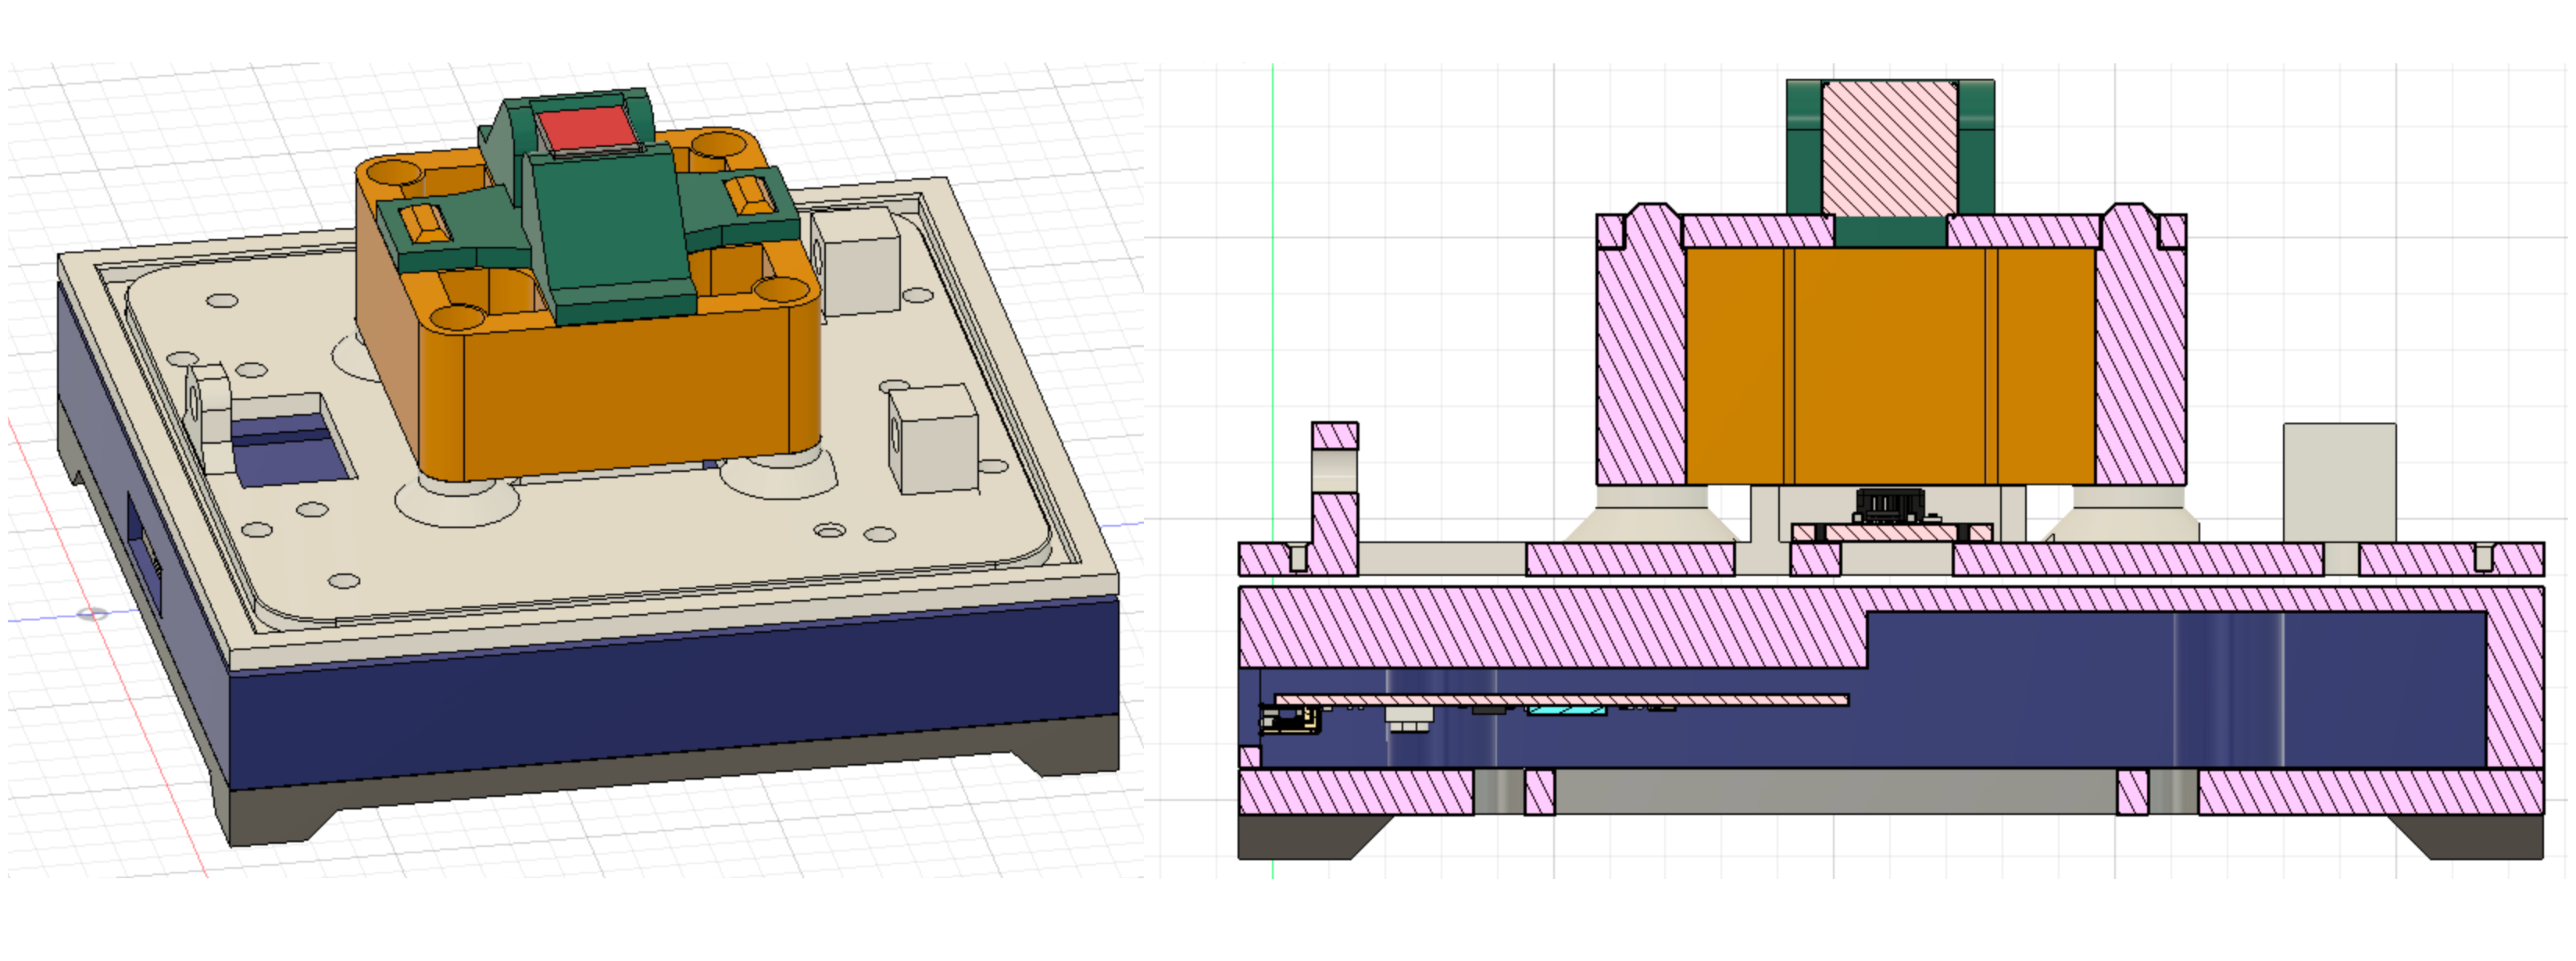
\includegraphics{./generated_images/border_Mechanical_components_for_the_1D_sensor_using_3D_printed_parts.png}
\caption{Mechanical components for the 1D sensor using 3D printed parts
\label{Mechanical_components_for_the_1D_sensor_using_3D_printed_parts.png}}
\end{figure}

The mechanical design of a sensor would be kept as simple as possible so
that it can be replicated as easily as possible. The focus was on
providing a stable foundation for the sensor \gls{ic} and an
exchangeable holder for different magnets.

The following figure
\ref{Mechanical_components_for_the_1D_sensor_using_3D_printed_parts.png},
shows a sectional view of the \gls{cad} drawing of the 1D-Single sensor
\ref{d-single-sensor}.

All parts were produced using the 3D printing additive manufacturing
processes. The sensor circuit board was glued underneath the magnet
holder. This is interchangeable, so different distances between sensor
and magnet can be realised.

The exchangeable magnetic holder (shown in green) can be adapted to
different magnets. It can be produced quickly due to the small amount of
parts used. The two recesses lock the magnet holder with the inserted
magnet over the sensor. The specified tolerances allow the magnet to be
inserted into the holder with repeat accuracy and without backlash. This
is important if several magnets have to be measured, where the
positioning over the sensor must always be the same.

\hypertarget{electrical-interface}{%
\section{Electrical Interface}\label{electrical-interface}}

\begin{figure}
\centering
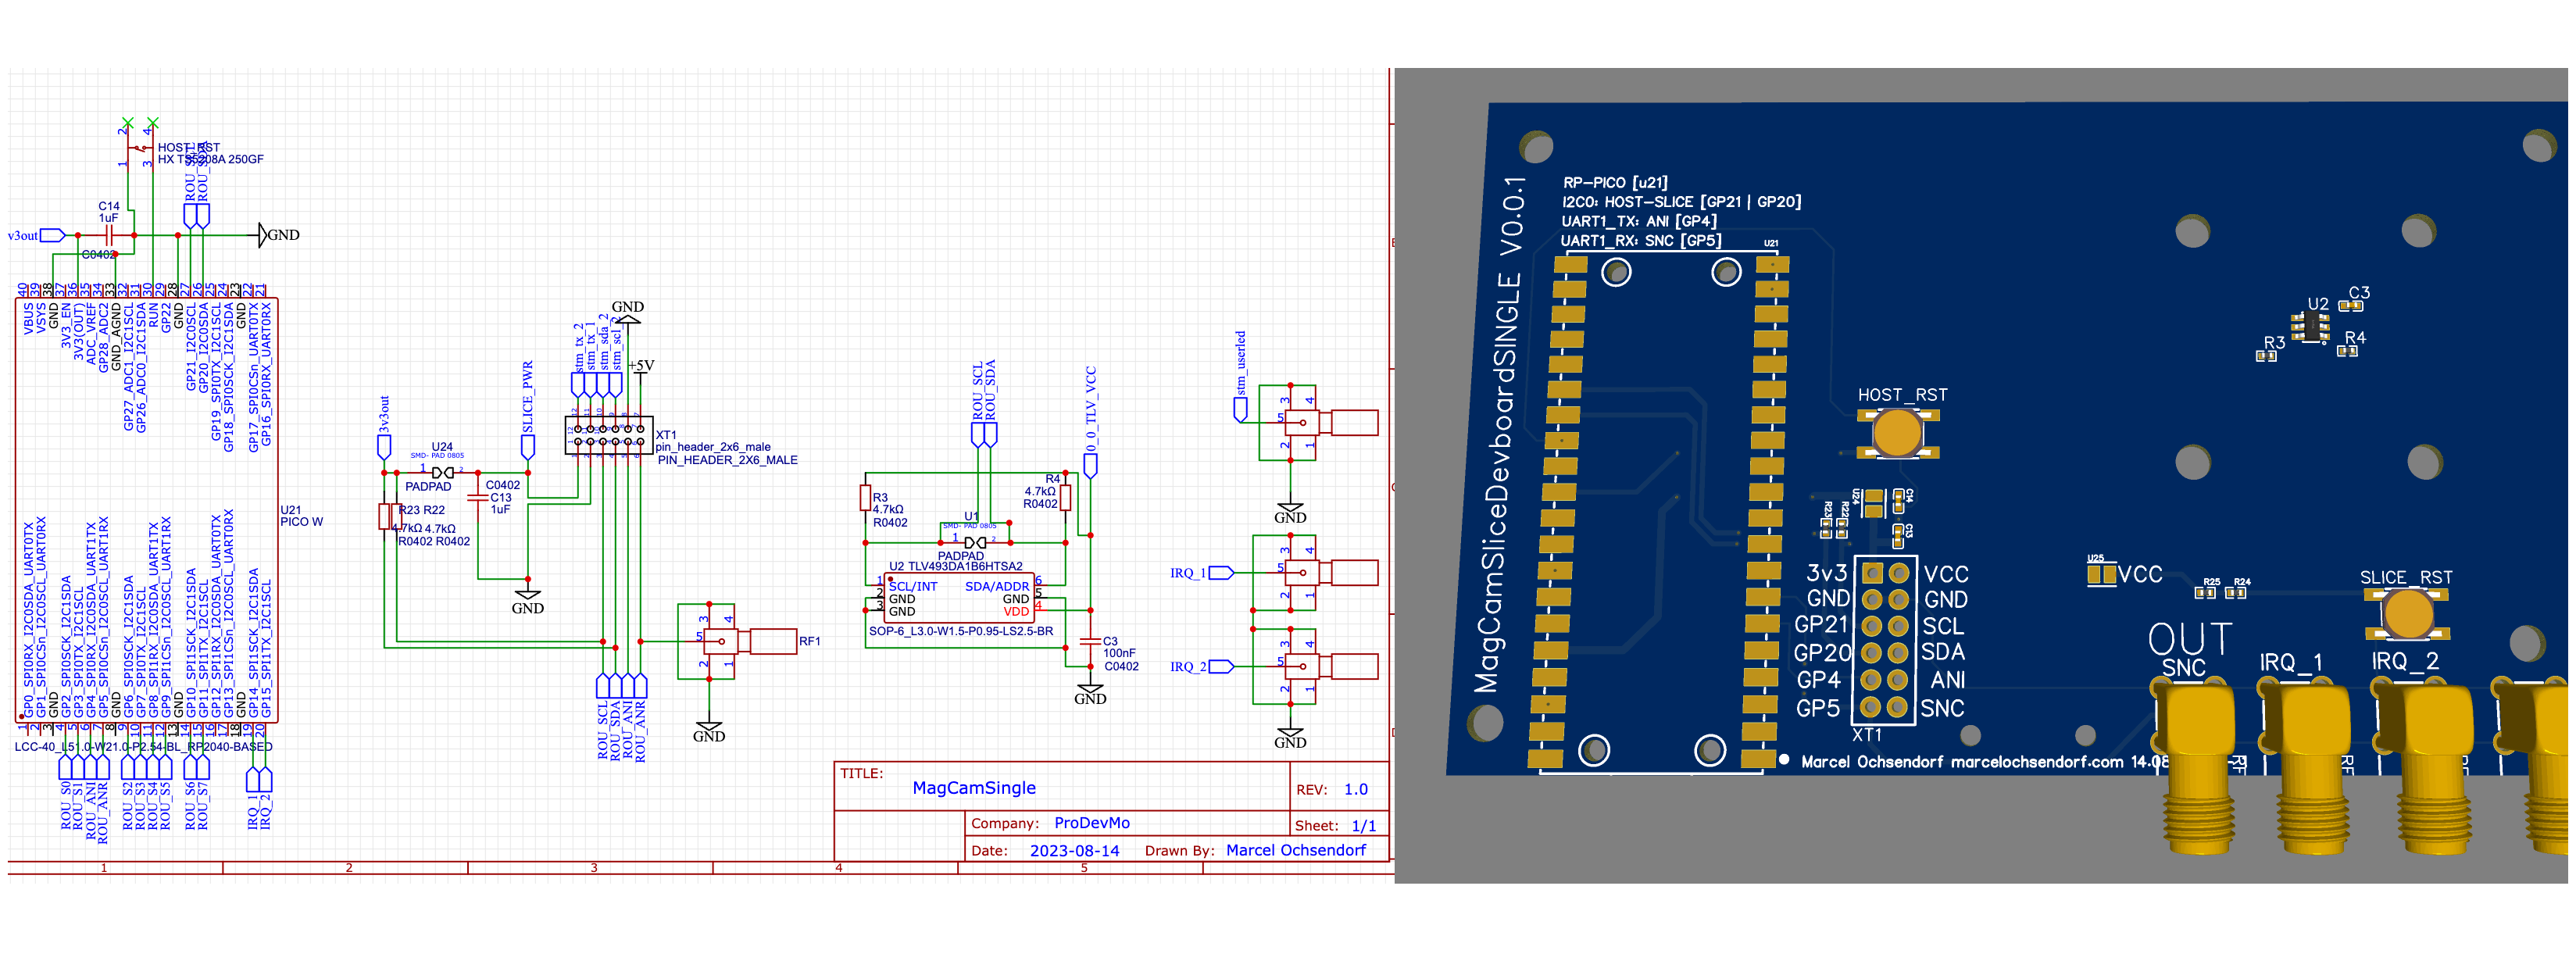
\includegraphics{./generated_images/border_1D_sensor_schematic_and_circuit_board.png}
\caption{1D sensor schematic and circuit board
\label{1D_sensor_schematic_and_circuit_board.png}}
\end{figure}

The electronics consist of the magnetic field sensor and the electrical
interface to connect it to a \gls{pc} in the form of a microcontroller.

The focus here was on utilising existing microcontroller development and
evaluation boards, which already integrate all the components required
for basic operation. This not only enabled a time-saving implementation,
but also ensured a cost-efficient realisation.

All the necessary components and their circuitry were then recorded on a
\gls{pcb} \ref{1D_sensor_schematic_and_circuit_board.png} and
subsequently manufactured. In addition, footprints were provided for
various sensor \gls{ic} packages. By placing mounting holes on the
\gls{pcb}, it is possible to attach various mechanical mounts ontop of
the sensor \gls{ic}s.

Special attention was paid to the provision of an accessible
SYNC-\gls{gpio} connector. This enables subsequent multi-sensor
synchronization and also offers options for later extensions. This
functionality opens up the possibility of synchronising data from
different sensors to achieve precise and coherent measurement results.
Overall, this integrated approach represents an effective solution for
the flexible evaluation of sensors and helps to optimise the development
process.

\hypertarget{firmware}{%
\section{Firmware}\label{firmware}}

\begin{figure}
\centering
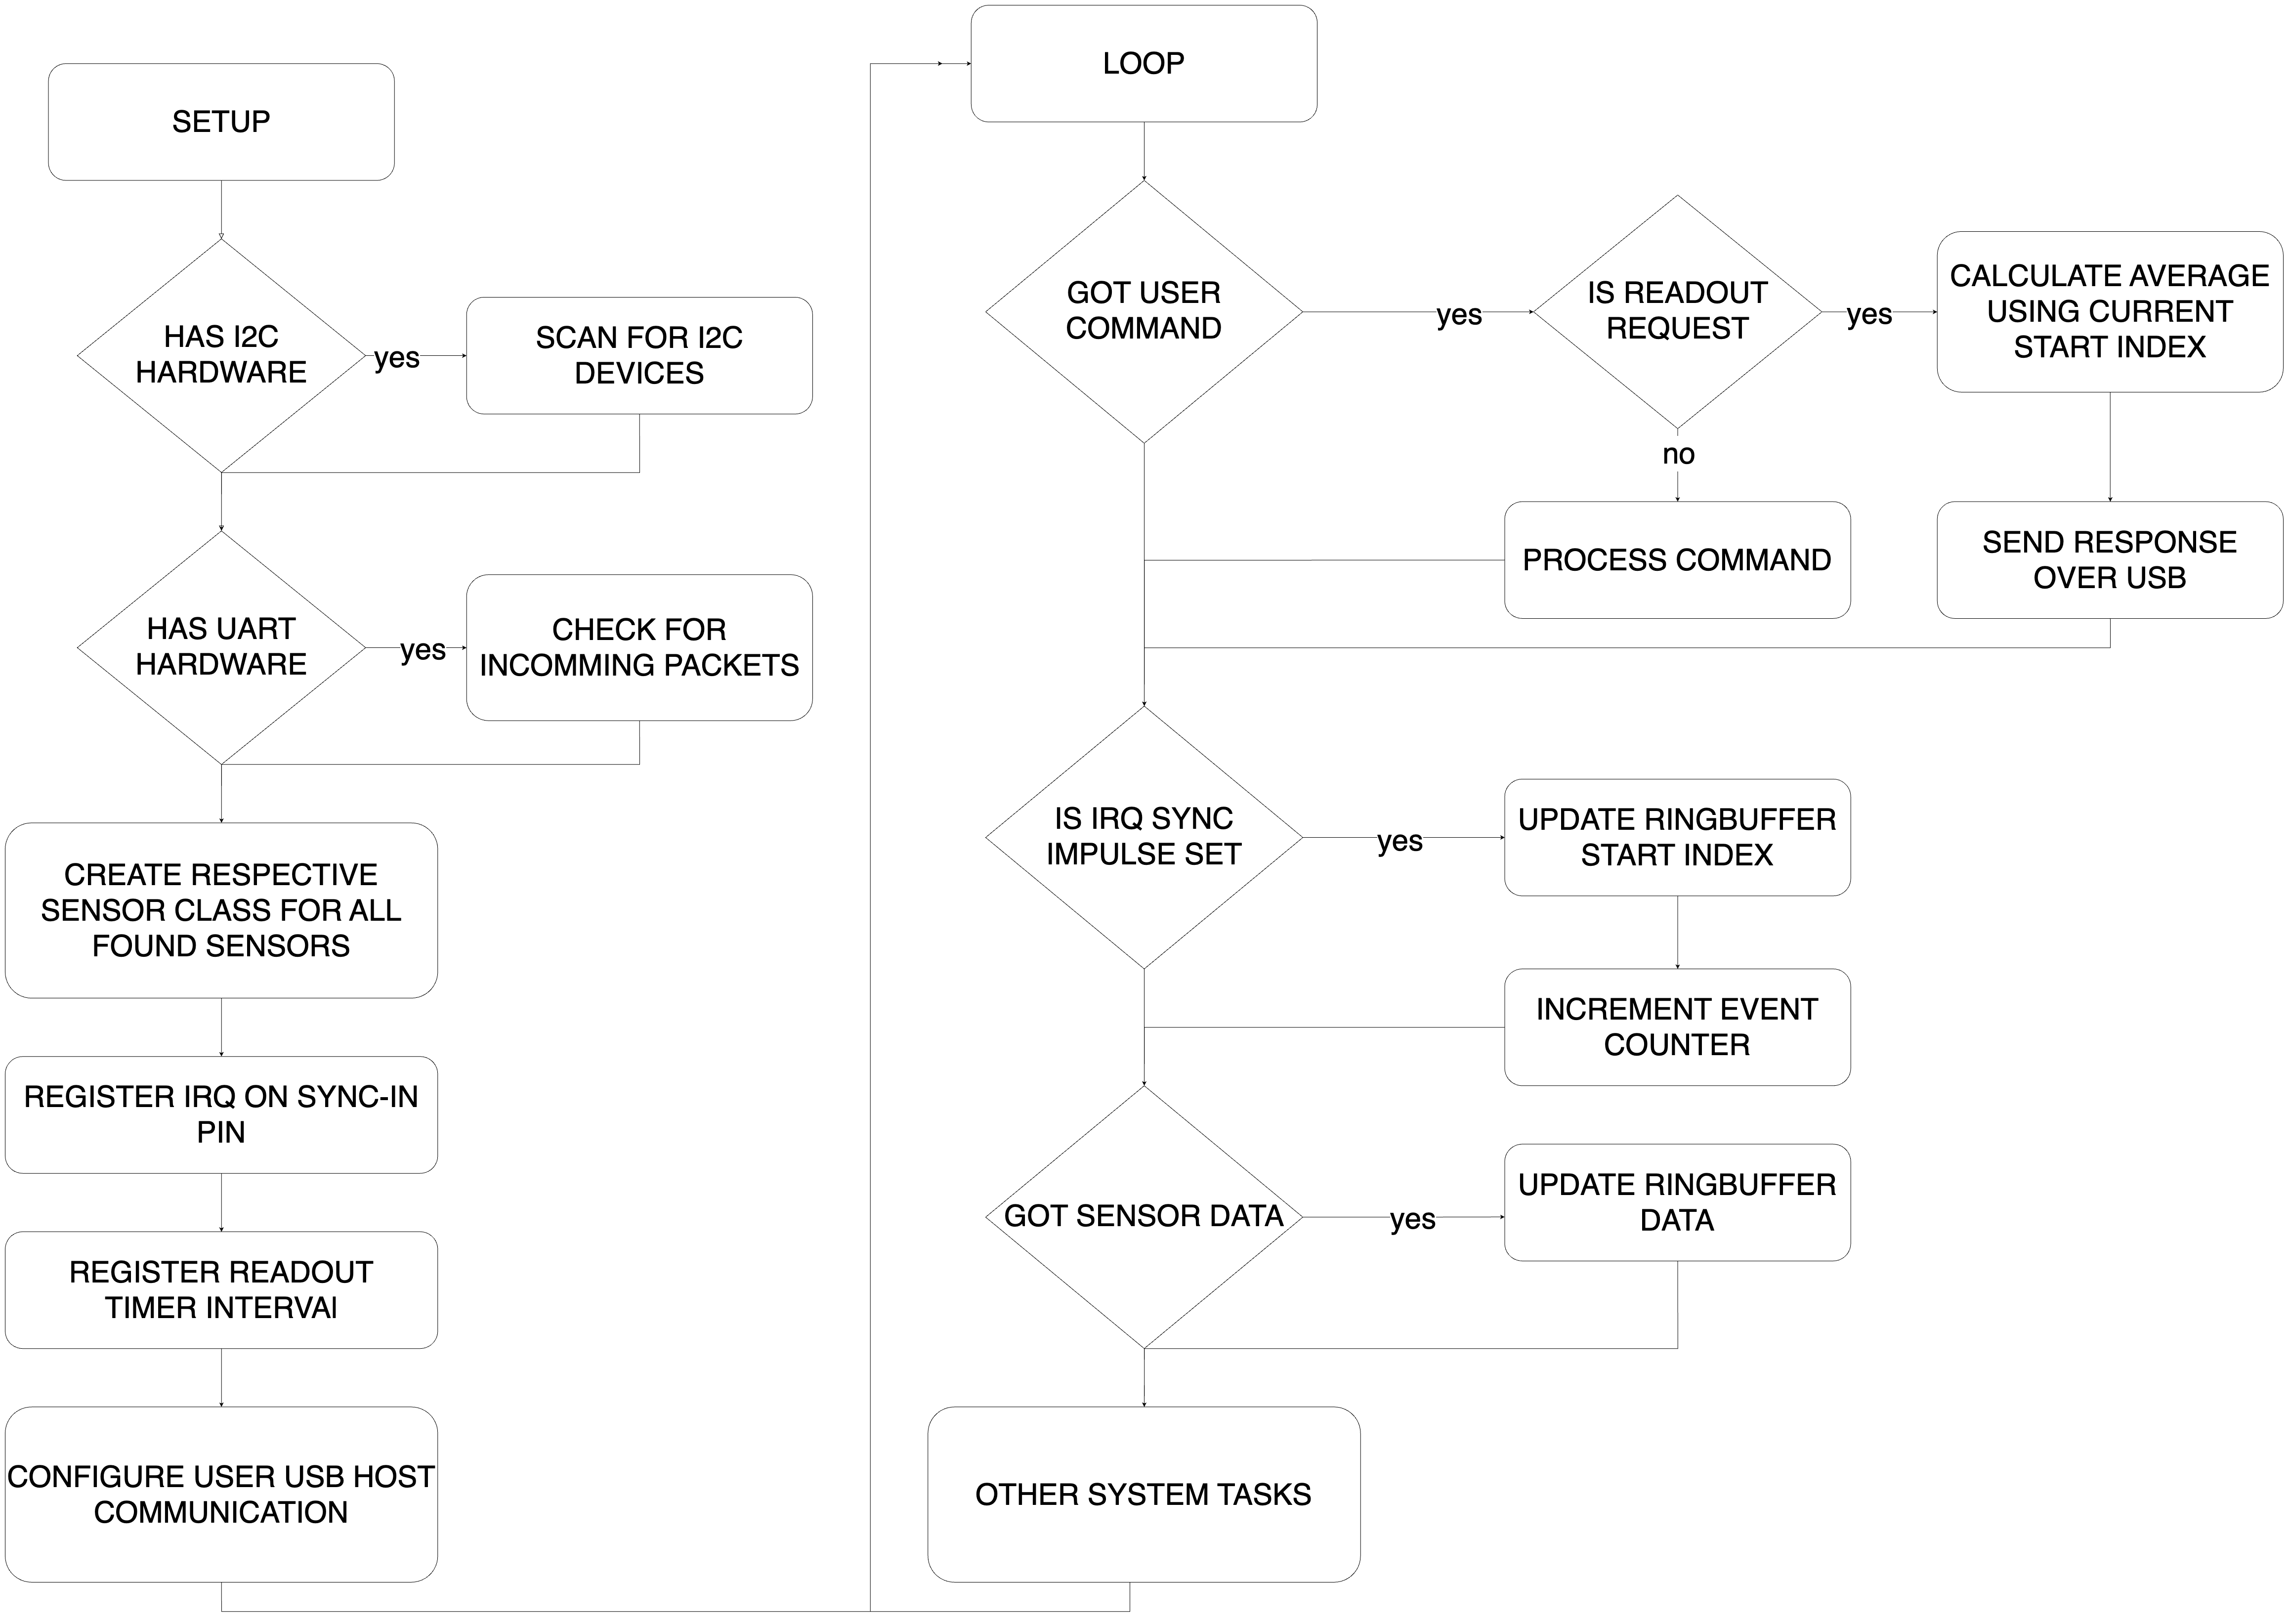
\includegraphics{./generated_images/border_Unified_sensor_firmware_simplified_program_structure.png}
\caption{Unified sensor firmware simplified program structure
\label{Unified_sensor_firmware_simplified_program_structure.png}}
\end{figure}

The microcontroller firmware is software that is executed on a
microcontroller in an embedded system. It controls the hardware and
enables the execution of predefined functions. The firmware is used to
process input data, control output devices and performs specific tasks
according to the program code.

It handles communication with sensors, actuators and other peripheral
devices, processing data and making decisions. Firmware is critical to
the functioning of devices.

The firmware is responsible for detecting the possible connected sensors
\ref{Implemented_digital_magnetic_field_sensors.csv} and query
measurements. This measured data can be forwarded to a host \gls{pc} via
a user interface and can then be further processed there.

An important component is that as many common sensors as possible can be
easily connected without having to adapt the firmware. This modularity
was implemented using abstract class design. These are initiated
according to the sensors found at startup. If new hardware is to be
integrated, only the required functions \ref{lst:CustomSensorClass} need
to be implemented.

\begin{lstlisting}[language={C++}, caption={CustomSensor-Class for adding new sensor hardware support}, label=lst:CustomSensorClass]
#ifndef __CustomSensor_h__
#define __CustomSensor_h__
// register your custom sensor in implemented_sensors.h also
class CustomSensor: public baseSensor
{
public:
  CustomSensor();
  ~CustomSensor();
  // implement depending sensor communication interface
  bool begin(TwoWire& _wire_instance); // I2C
  bool begin(HardwareSerial& _serial_instance); // UART
  bool begin(Pin& _pin_instance); // ANALOG or DIGITAL PIN like onewire
  // FUNCTIONS USED BY READOUT LOGIC
  bool is_valid() override;
  String capabilities() override;
  String get_sensor_name() override;
  bool query_sensor() override;
  sensor_result get_result() override;        
};
#endif
\end{lstlisting}

The flow chart
\ref{Unified_sensor_firmware_simplified_program_structure.png} shows the
start process and the subsequent main loop for processing the user
commands and sensor results. When the microcontroller is started, the
software checks whether known sensors are connected to \gls{i2c} or
\gls{uart} interfaces.

If any are found (using a dedicated \gls{lut} with sensor address
translation information), the appropriate class instances are created
and these can later be used to read out measurement results.

The next initialisation system is dedicated for multi-sensor
synchronisation \ref{sensor-syncronisation-interface}. The last step in
the setup is to configure communication with the host or connected
\gls{pc}. All implemented microcontroller platforms used (Raspberry Pi
Pico, STM32F4) have a \gls{usb} slave port.

The used usb descriptor is a \gls{usb} \gls{cdc}. This is used to
emulate a virtual RS232 communication port using a \gls{usb} port on a
\gls{pc} and usually no additional driver is needed on modern host
systems.

After execution of the setup routine is completed, the system switches
to an infinite loop, which processes several possible actions. One task
is, to react to user commands which can be sent to the system by the
user via the integrated \gls{cli}. All sensors are read out via a timer
interval set in the setup procedure and their values are stored in a
ringbuffer. Ring buffer offers efficient data management in limited
memory. Its cyclic structure enables continuous overwriting of older
data, saves memory space and facilitates seamless processing of
real-time data.

Ring buffers are well suited for applications with variable data rates
and minimise the need for complex memory management. The buffer can be
read out by command and the result of the measurement is sent to the
host. Each sensor measurement result is transmitted from the buffer to
the host together with a time stamp and a sequential number. This
ensures that in a multi-sensor setup with several sensors. The
measurements are synchronized \ref{sensor-syncronisation-interface} in
time and are not out of sequence or drift.

\hypertarget{communication-interface}{%
\subsection{Communication Interface}\label{communication-interface}}

\begin{figure}
\centering
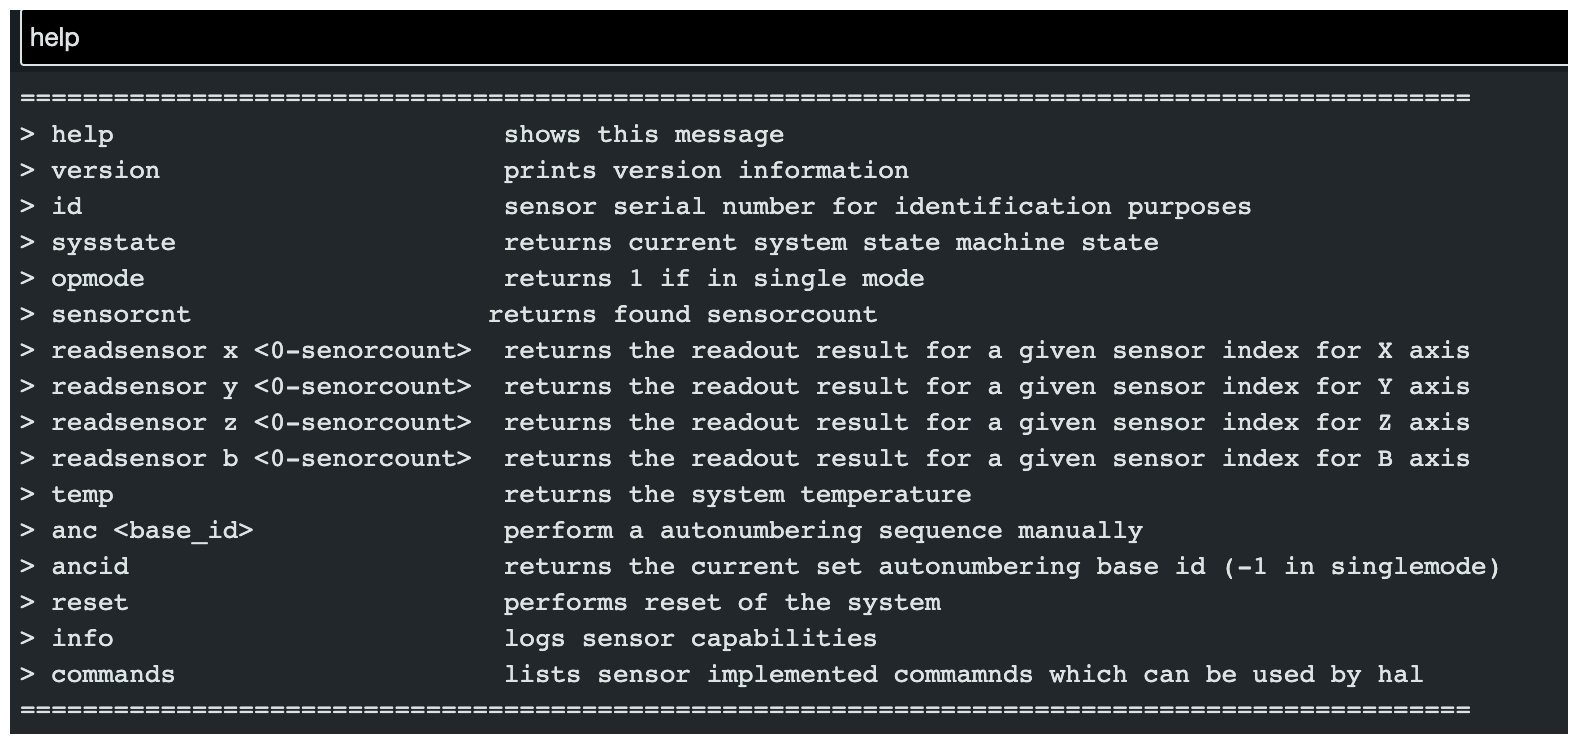
\includegraphics{./generated_images/border_Sensors_(+cli).png}
\caption{Sensors \gls{cli} \label{Sensors_(+cli).png}}
\end{figure}

Each sensor that has been loaded with the firmware, registeres on to the
host \gls{pc} as a serial interface. There are several ways for the user
to interact with the sensor:

\begin{itemize}
\tightlist
\item
  Use with \gls{mrp} \ref{software-readout-framework}-libaray
\item
  Stand-alone mode via sending commands using built-in \gls{cli}
\end{itemize}

The \gls{cli} mode is a simple text-based interface with which it is
possible to read out current measured values, obtain debug information
and set operating parameters. This allows to quickly determine whether
the hardware is working properly after installation. The \gls{cli}
behaves like terminal programmes, displaying a detailed command
reference \ref{Sensors_(+cli).png} to the user after connecting. The
current measured value can be output using the
\passthrough{\lstinline!readout!} command
\ref{Query_sensors_b_value_using_(+cli).png}.

\begin{figure}
\centering
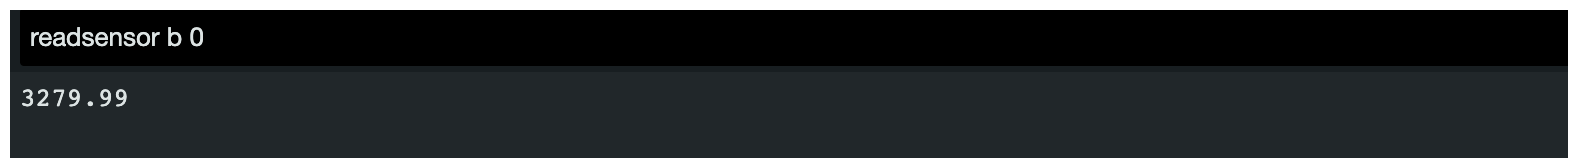
\includegraphics{./generated_images/border_Query_sensors_b_value_using_(+cli).png}
\caption{Query sensors b value using \gls{cli}
\label{Query_sensors_b_value_using_(+cli).png}}
\end{figure}

The other option is to use the \gls{mrp}
\ref{software-readout-framework}-library. The serial interface is also
used here. However, after a connection attempt by the \gls{hal}
\ref{mrphal} module of the \gls{mrp}
\ref{software-readout-framework}-library, the system switches to binary
mode, which is initiated using the \passthrough{\lstinline!sbm!}
command. The same commands are available as for \gls{cli}-based
communication, but in a binary format.

\hypertarget{sensor-syncronisation-interface}{%
\subsection{Sensor Syncronisation
Interface}\label{sensor-syncronisation-interface}}

\begin{figure}
\centering
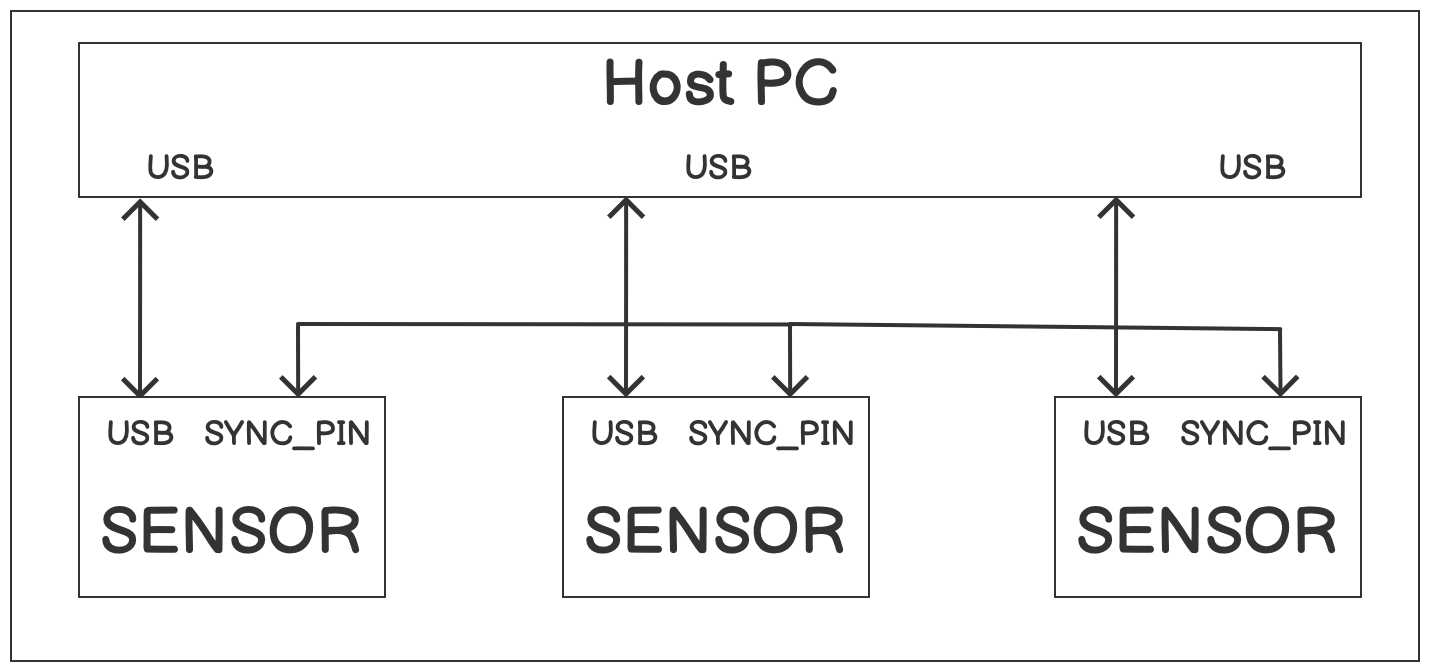
\includegraphics{./generated_images/border_Multi_sensor_synchronisation_wiring_example.png}
\caption{Multi sensor synchronisation wiring example
\label{Multi_sensor_synchronisation_wiring_example.png}}
\end{figure}

One problem with the use of several sensors on one readout host \gls{pc}
is that the measurements may drift over time. On the one hand, \gls{usb}
latencies can occur. This can occur due to various factors, including
device drivers, data transfer speed and system resources. High-quality
\gls{usb} devices and modern drivers often minimise latencies.
Nevertheless, complex data processing tasks and overloaded \gls{usb}
ports can lead to delays.

\begin{longtable}[]{@{}lllll@{}}
\caption{Measured sensor readout to processing using host software
\label{Measured_sensor_readout_to_processing_using_host_software.csv}}\tabularnewline
\toprule
\begin{minipage}[b]{0.08\columnwidth}\raggedright
Data-Points\strut
\end{minipage} & \begin{minipage}[b]{0.11\columnwidth}\raggedright
Run runtime {[}ms{]}\strut
\end{minipage} & \begin{minipage}[b]{0.35\columnwidth}\raggedright
Average Sensor communication time per reading {[}ms{]}\strut
\end{minipage} & \begin{minipage}[b]{0.22\columnwidth}\raggedright
Communication jitter time {[}ms{]}\strut
\end{minipage} & \begin{minipage}[b]{0.10\columnwidth}\raggedright
Comment\strut
\end{minipage}\tabularnewline
\midrule
\endfirsthead
\toprule
\begin{minipage}[b]{0.08\columnwidth}\raggedright
Data-Points\strut
\end{minipage} & \begin{minipage}[b]{0.11\columnwidth}\raggedright
Run runtime {[}ms{]}\strut
\end{minipage} & \begin{minipage}[b]{0.35\columnwidth}\raggedright
Average Sensor communication time per reading {[}ms{]}\strut
\end{minipage} & \begin{minipage}[b]{0.22\columnwidth}\raggedright
Communication jitter time {[}ms{]}\strut
\end{minipage} & \begin{minipage}[b]{0.10\columnwidth}\raggedright
Comment\strut
\end{minipage}\tabularnewline
\midrule
\endhead
\begin{minipage}[t]{0.08\columnwidth}\raggedright
1\strut
\end{minipage} & \begin{minipage}[t]{0.11\columnwidth}\raggedright
9453\strut
\end{minipage} & \begin{minipage}[t]{0.35\columnwidth}\raggedright
1.44\strut
\end{minipage} & \begin{minipage}[t]{0.22\columnwidth}\raggedright
0\strut
\end{minipage} & \begin{minipage}[t]{0.10\columnwidth}\raggedright
\strut
\end{minipage}\tabularnewline
\begin{minipage}[t]{0.08\columnwidth}\raggedright
1\strut
\end{minipage} & \begin{minipage}[t]{0.11\columnwidth}\raggedright
9864\strut
\end{minipage} & \begin{minipage}[t]{0.35\columnwidth}\raggedright
1.5\strut
\end{minipage} & \begin{minipage}[t]{0.22\columnwidth}\raggedright
0\strut
\end{minipage} & \begin{minipage}[t]{0.10\columnwidth}\raggedright
\strut
\end{minipage}\tabularnewline
\begin{minipage}[t]{0.08\columnwidth}\raggedright
10\strut
\end{minipage} & \begin{minipage}[t]{0.11\columnwidth}\raggedright
12984\strut
\end{minipage} & \begin{minipage}[t]{0.35\columnwidth}\raggedright
1.22\strut
\end{minipage} & \begin{minipage}[t]{0.22\columnwidth}\raggedright
0.9\strut
\end{minipage} & \begin{minipage}[t]{0.10\columnwidth}\raggedright
\strut
\end{minipage}\tabularnewline
\begin{minipage}[t]{0.08\columnwidth}\raggedright
10\strut
\end{minipage} & \begin{minipage}[t]{0.11\columnwidth}\raggedright
12673\strut
\end{minipage} & \begin{minipage}[t]{0.35\columnwidth}\raggedright
1.13\strut
\end{minipage} & \begin{minipage}[t]{0.22\columnwidth}\raggedright
1.1\strut
\end{minipage} & \begin{minipage}[t]{0.10\columnwidth}\raggedright
\strut
\end{minipage}\tabularnewline
\begin{minipage}[t]{0.08\columnwidth}\raggedright
10\strut
\end{minipage} & \begin{minipage}[t]{0.11\columnwidth}\raggedright
43264\strut
\end{minipage} & \begin{minipage}[t]{0.35\columnwidth}\raggedright
2.19\strut
\end{minipage} & \begin{minipage}[t]{0.22\columnwidth}\raggedright
8.2\strut
\end{minipage} & \begin{minipage}[t]{0.10\columnwidth}\raggedright
96\% system load\strut
\end{minipage}\tabularnewline
\bottomrule
\end{longtable}

The table
shows\ref{Measured_sensor_readout_to_processing_using_host_software.csv}
shows various jitter measurements. These were performed on a
\passthrough{\lstinline!RaspberryPi 4 4GB!}-\gls{sbc} together with an
\passthrough{\lstinline!1D: Single Sensor!} \ref{d-single-sensor} and
the following software settings:

\begin{itemize}
\tightlist
\item
  Raspberry Pi OS Lite - \gls{os}
  \passthrough{\lstinline!debian bookworm x64!},
\item
  \gls{mrp} \ref{software-readout-framework}-library - Version
  \passthrough{\lstinline!1.4.1!}
\item
  Unified Sensor \ref{unified-sensor}-firmware - Version
  \passthrough{\lstinline!1.0.1!}
\end{itemize}

It can be seen that a jitter time of up to an additional
\passthrough{\lstinline!1ms!} is added between the triggering of the
measurements by the host system and the receipt of the command by the
sensor hardware. If the host system is still under load, this value
increases many times over. This means that synchronising several sensors
via the \gls{usb} connection alone is not sufficient.

The other issue is sending the trigger signal from the readout software
\ref{software-readout-framework}. Here too, unpredictable latencies can
occur, depending on which other tasks are also executed on this port.

In order to enable the most stable possible synchronisation between
several sensors, an option has already been created to establish an
electrical connection between sensors. This is used together with the
firmware to synchronise the readout intervals. The schematic
\ref{Multi_sensor_synchronisation_wiring_example.png} shows how several
sensors must be wired together in order to implement this form of
synchronisation.

\begin{figure}
\centering
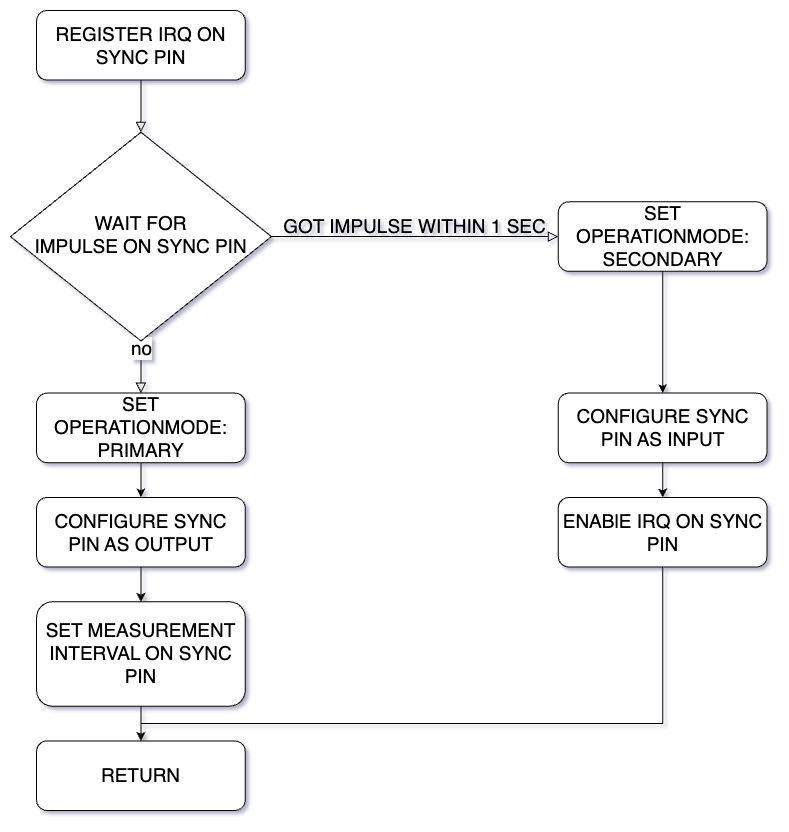
\includegraphics{./generated_images/border_Unified_sensor_firmware_multi_sensor_synchronisation_procedure.png}
\caption{Unified sensor firmware multi sensor synchronisation procedure
\label{Unified_sensor_firmware_multi_sensor_synchronisation_procedure.png}}
\end{figure}

Once the hardware has been prepared, the task of the firmware of the
various sensors is to find a common synchronisation clock. To do this,
the function \passthrough{\lstinline!register irq on sync pin!} is
overwritten. To set one \passthrough{\lstinline!primary!} and several
\passthrough{\lstinline!secondary!} sensors, each sensor waits for an
intial pulse on the SYNC-\gls{gpio}
\ref{Unified_sensor_firmware_multi_sensor_synchronisation_procedure.png}.
Each sensor starts a random timer beforehand, which sends a pulse on the
sync line. All others receive this and switch to
\passthrough{\lstinline!secondary!} mode and synchronise the
measurements based on each sync pulse received.

Since the presumed \passthrough{\lstinline!primary!} sensor cannot
register its own sync pulse (because the pin is switched to output),
there is a timeout branch condition
\passthrough{\lstinline!got pulse within 1000ms!} and this becomes the
\passthrough{\lstinline!primary!} sensor. This means that in a chain of
sensors there is exactly one \passthrough{\lstinline!primary!} and many
\passthrough{\lstinline!secondary!} sensors.

In single-sensor operation, this automatically jumps to
\passthrough{\lstinline!primary!} sensor operation through the
\passthrough{\lstinline!got impulse within 1000ms!} branch result. The
synchronisation status can be queried via the user interface
\ref{communication-interface} using the \passthrough{\lstinline!opmode!}
\ref{Query_opmode_using_(+cli).png} command. An important aspect of the
implementation here was that there is no numbering or sequence of the
individual sensors.

This means that for the subsequent readout of the measurements, it is
only important that they are taken at the same interval across all
sensors. The sensor differentiation takes place later in the \gls{mrp}
\ref{software-readout-framework}-library by using the sensor \gls{uuid}.

\begin{figure}
\centering
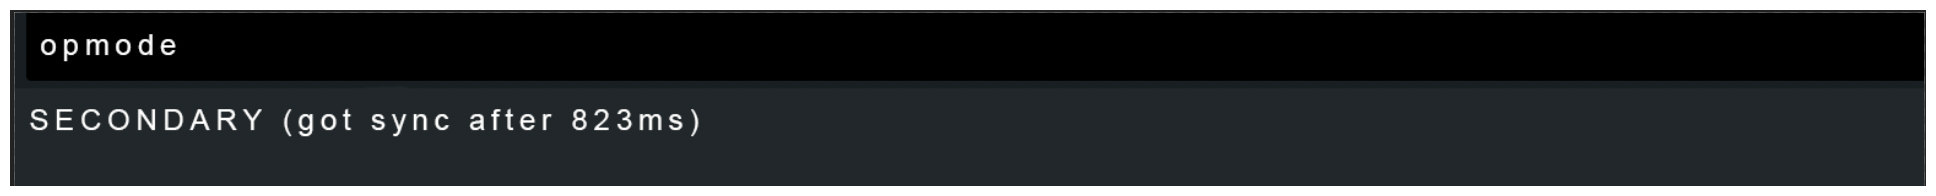
\includegraphics{./generated_images/border_Query_opmode_using_(+cli).png}
\caption{Query opmode using \gls{cli}
\label{Query_opmode_using_(+cli).png}}
\end{figure}

\hypertarget{example-sensors}{%
\section{Example Sensors}\label{example-sensors}}

Two functional sensor platforms
\ref{Build_sensors_with_different_capabilities.csv} were built in order
to create a solid test platform for later tests and for the development
of the \gls{mrp} \ref{software-readout-framework}-library with the
previously developed sensor concepts.

\begin{longtable}[]{@{}llll@{}}
\caption{Build sensors with different capabilities
\label{Build_sensors_with_different_capabilities.csv}}\tabularnewline
\toprule
& 1D\ref{d-single-sensor} & 1D: dual sensor & 3D:
Fullsphere\ref{d-fullsphere}\tabularnewline
\midrule
\endfirsthead
\toprule
& 1D\ref{d-single-sensor} & 1D: dual sensor & 3D:
Fullsphere\ref{d-fullsphere}\tabularnewline
\midrule
\endhead
Maximal magnet size & Cubic 30x30x30 & Cubic 30x30x30 & Cubic
20x20x20\tabularnewline
Sensor type & MMC5603NJ & TLV493D & TLV493D\tabularnewline
Sensor count & 1 & 2 & 1\tabularnewline
Scanmode & static (1 point) & static (2 points) & dynamic
(fullsphere)\tabularnewline
\bottomrule
\end{longtable}

These cover all the required functions described in the usecases
\ref{usecases}. The most important difference, apart from the sensor
used, is the \passthrough{\lstinline!scan mode!}. In this context, this
describes whether the sensor can measure a
\passthrough{\lstinline!static!} fixed point on the magnet or if the
sensor can move \passthrough{\lstinline!dynamically!} around the magnet
using a controllable manipulator.

In the following, the hardware structure of a
\passthrough{\lstinline!static!} and \passthrough{\lstinline!dynamic!}
sensor is described. For the \passthrough{\lstinline!static!} sensor,
only the \passthrough{\lstinline!1D!} variant is shown, as this does not
differ significantly from the structure of the
\passthrough{\lstinline!1D: dual sensor!}, except it uses two
\passthrough{\lstinline!TLV493D!} sensors, mounted above and on top of
the magnet.

\hypertarget{d-single-sensor}{%
\subsection{1D: Single Sensor}\label{d-single-sensor}}

\begin{figure}
\centering
\includegraphics{./generated_images/border_1D_sensor_construction_with_universal_magnet_mount.png}
\caption{1D sensor construction with universal magnet mount
\label{1D_sensor_construction_with_universal_magnet_mount.png}}
\end{figure}

The 1D sensor
\ref{1D_sensor_construction_with_universal_magnet_mount.png} is the
simplest possible sensor that is compatible with the Unified Sensor
firmware \ref{firmware} platform.

The electrical level here is based on a
\passthrough{\lstinline!Raspberry-Pi Pico!} together with the
\passthrough{\lstinline!MMC5603NJ!} magnetic sensor. The mechanical
setup consists of four 3D printed components, which are fixed together
with nylon screws to minimise possible influences on the measurement.

Since the \passthrough{\lstinline!MMC5603NJ!} only has limited
measurement range of total 6uT, even small coin sized neodymium magnets
already saturates the sensor. It is possible to mount 3D printed spacers
over the sensor to increase the distance between the magnet and the
sensor and thus also measure these magnets.

The designed magnet holder can be adapted for different magnet shapes
and can be placed on the spacer without backlash in order to be able to
perform a repeatable measurement without introducing measurement
irregularities by mechanically changing the magnet.

\hypertarget{d-fullsphere}{%
\subsection{3D: Fullsphere}\label{d-fullsphere}}

\begin{figure}
\centering
\includegraphics{./generated_images/border_Full-Sphere_sensor_implementation_using_two_Nema17_stepper_motors_in_a_polar_coordinate_system.png}
\caption{Full-Sphere sensor implementation using two Nema17 stepper
motors in a polar coordinate system
\label{Full-Sphere_sensor_implementation_using_two_Nema17_stepper_motors_in_a_polar_coordinate_system.png}}
\end{figure}

The 3D fullsphere sensor
\ref{Full-Sphere_sensor_implementation_using_two_Nema17_stepper_motors_in_a_polar_coordinate_system.png}
offers the possibility to create a 3D map of the inserted magnet.

The graphic
\ref{3D_plot_of_an_N45_12x12x12_magnet_using_the_3D_fullsphere_sensor.png}
shows the visualisation of such a scan in the form of a spherical 3D
map. On the sphere is the magnetic field strength, which was detected by
the sensor at the position. The transition from a fully positive field
strength (red) to a negative field strength (blue) is clearly
recognisable and corresponds to the orientation of the magnet in the
holder.

The magnet sensor is mounted on a movable arm, which can move 180
degrees around the magnet on one axis. In order to be able to map the
full sphere, the magnet is mounted on a turntable. This permits the
manipulator to move a polar coordinate system.

\begin{figure}
\centering
\includegraphics{./generated_images/border_3D_plot_of_an_N45_12x12x12_magnet_using_the_3D_fullsphere_sensor.png}
\caption{3D plot of an N45 12x12x12 magnet using the 3D fullsphere
sensor
\label{3D_plot_of_an_N45_12x12x12_magnet_using_the_3D_fullsphere_sensor.png}}
\end{figure}

As the magnets in the motors, as with the screws used in the 1D sensor,
can influence the measurements of the magnetic field sensor, the
distance between these components and the sensor or magnets was
increased. The turntable and its drive motor are connected to each other
via a belt.

On the electrical side, it also consists of a
\passthrough{\lstinline!SKR-Pico!} stepper motor controller, together
with the \passthrough{\lstinline!TLV493D!} magnetic field sensor. This
was chosen because of its larger measuring range and can therefore be
used more universally without having to change the sensor of the arm.

\hypertarget{integration-of-an-industry-teslameter}{%
\subsection{Integration of an
Industry-Teslameter}\label{integration-of-an-industry-teslameter}}

As the sensors shown so far relate exclusively to self-built, low-cost
hardware, the following section shows how existing hardware can be
integrated into the system. A temperature-compensated
\passthrough{\lstinline!Voltcraft GM-70!} telsameter
\ref{Voltcraft_GM70_teslameter_with_custom_(+pc)_interface_board.png} is
used, which has a measuring range of 0T to 3T with a resolution of
0.1mT. It offers an RS232 interface with a documented protocol
\ref{Voltcraft_GM70_serial_protocol.csv} for connection to a \gls{pc}.

This connectivity makes it possible to make the device compatible with
the unified sensor ecosystem using a separate interface software
\cite{VoltcraftGM70Rest} executable on the host \gls{pc}. However,
it does not offer the range of functions that the unified sensor
firmware offers.

Another option is a custom interface board between the meter and the PC.
This is a good option as many modern \gls{pc}s or \gls{sbc}s no longer
offer an physical RS232 interface. As with the other sensors, this
interface consists of your \passthrough{\lstinline!Raspberry-Pi Pico!}
with an additional level shifter.

The teslameter is connected to the microcontroller using two free
\gls{gpio}s in \gls{uart} mode. The firmware was adapted using a
separate build configuration. In order to be able to read and correctly
interpret the data from the microcontoller, the serial protocol from
table \ref{Voltcraft_GM70_serial_protocol.csv} of the sensor was
implemented in a customized version of the
\passthrough{\lstinline!CustomSensor!} class
\ref{lst:CustomSensorClass}.

This software or hardware integration can be carried out on any other
measuring device with a suitable communication interface and a known
protocol thanks to the modular design.

\begin{figure}
\centering
\includegraphics{./generated_images/border_Voltcraft_GM70_teslameter_with_custom_(+pc)_interface_board.png}
\caption{Voltcraft GM70 teslameter with custom \gls{pc} interface board
\label{Voltcraft_GM70_teslameter_with_custom_(+pc)_interface_board.png}}
\end{figure}

\begin{longtable}[]{@{}lll@{}}
\caption{Voltcraft GM70 serial protocol
\label{Voltcraft_GM70_serial_protocol.csv}}\tabularnewline
\toprule
BYTE-INDEX & REPRESENTATION & VALUE\tabularnewline
\midrule
\endfirsthead
\toprule
BYTE-INDEX & REPRESENTATION & VALUE\tabularnewline
\midrule
\endhead
0 & PREAMBLE & 0x2\tabularnewline
1 & & 0x1\tabularnewline
2 & & 0x4\tabularnewline
3 & UNIT & `B' =\textgreater{} Gauss `E' =\textgreater{}
mT\tabularnewline
5 & POLARITY & `1' =\textgreater{} \emph{0.1 `2' =\textgreater{}
}0.01\tabularnewline
6 & value MSB & 0x-0xFF\tabularnewline
13 & value LSB & 0x-0xFF\tabularnewline
14 & STOP & 0x3\tabularnewline
\bottomrule
\end{longtable}

\hypertarget{software-readout-framework}{%
\chapter{Software Readout Framework}\label{software-readout-framework}}

The software readout framework is the central software component that
was developed as part of this work. This software framework is intended
to provide a user-oriented data acquisition and analysis environment.
For this purpose, typical individual steps that occur in relation to
these tasks were implemented:

\begin{itemize}
\tightlist
\item
  Data acquisition - from hardware sensors \ref{unified-sensor} or other
  data sources
\item
  Storage - export of data in various open formats
  \ref{storage-and-datamanagement}
\item
  Analysis - algorithms to analyze different data sets \ref{analysis}
\end{itemize}

All these possible task parts were divided into different blocks and
users were given the possibility of adding their own functionalities.

As the following, this concept is referred to as
\passthrough{\lstinline!user interaction points!}
\ref{user-interaction-points} and is explained in the following chapter.

\hypertarget{user-interaction-points}{%
\section{User Interaction Points}\label{user-interaction-points}}

User interaction points represent the core concept of the developed
library and are intended to provide user-friendliness on the one hand
and the rapid development of own analysis and optimization algorithms on
the other.

For this purpose, the library was divided into individual modules, which
are shown in the graphic
\ref{MRP_library_module_high_level_overview.png}. In combination, these
represent a typical measurement-analysis-evaluation workflow of data.
For this purpose, a module system with standardised functional patterns
and data types was developed and packed together in a extendable Python
library.

\newpage

According to this concept, the user should be able to replace individual
components from this chain with their own modules without having to
worry about implementing other of these to make the project work.

\begin{figure}
\centering
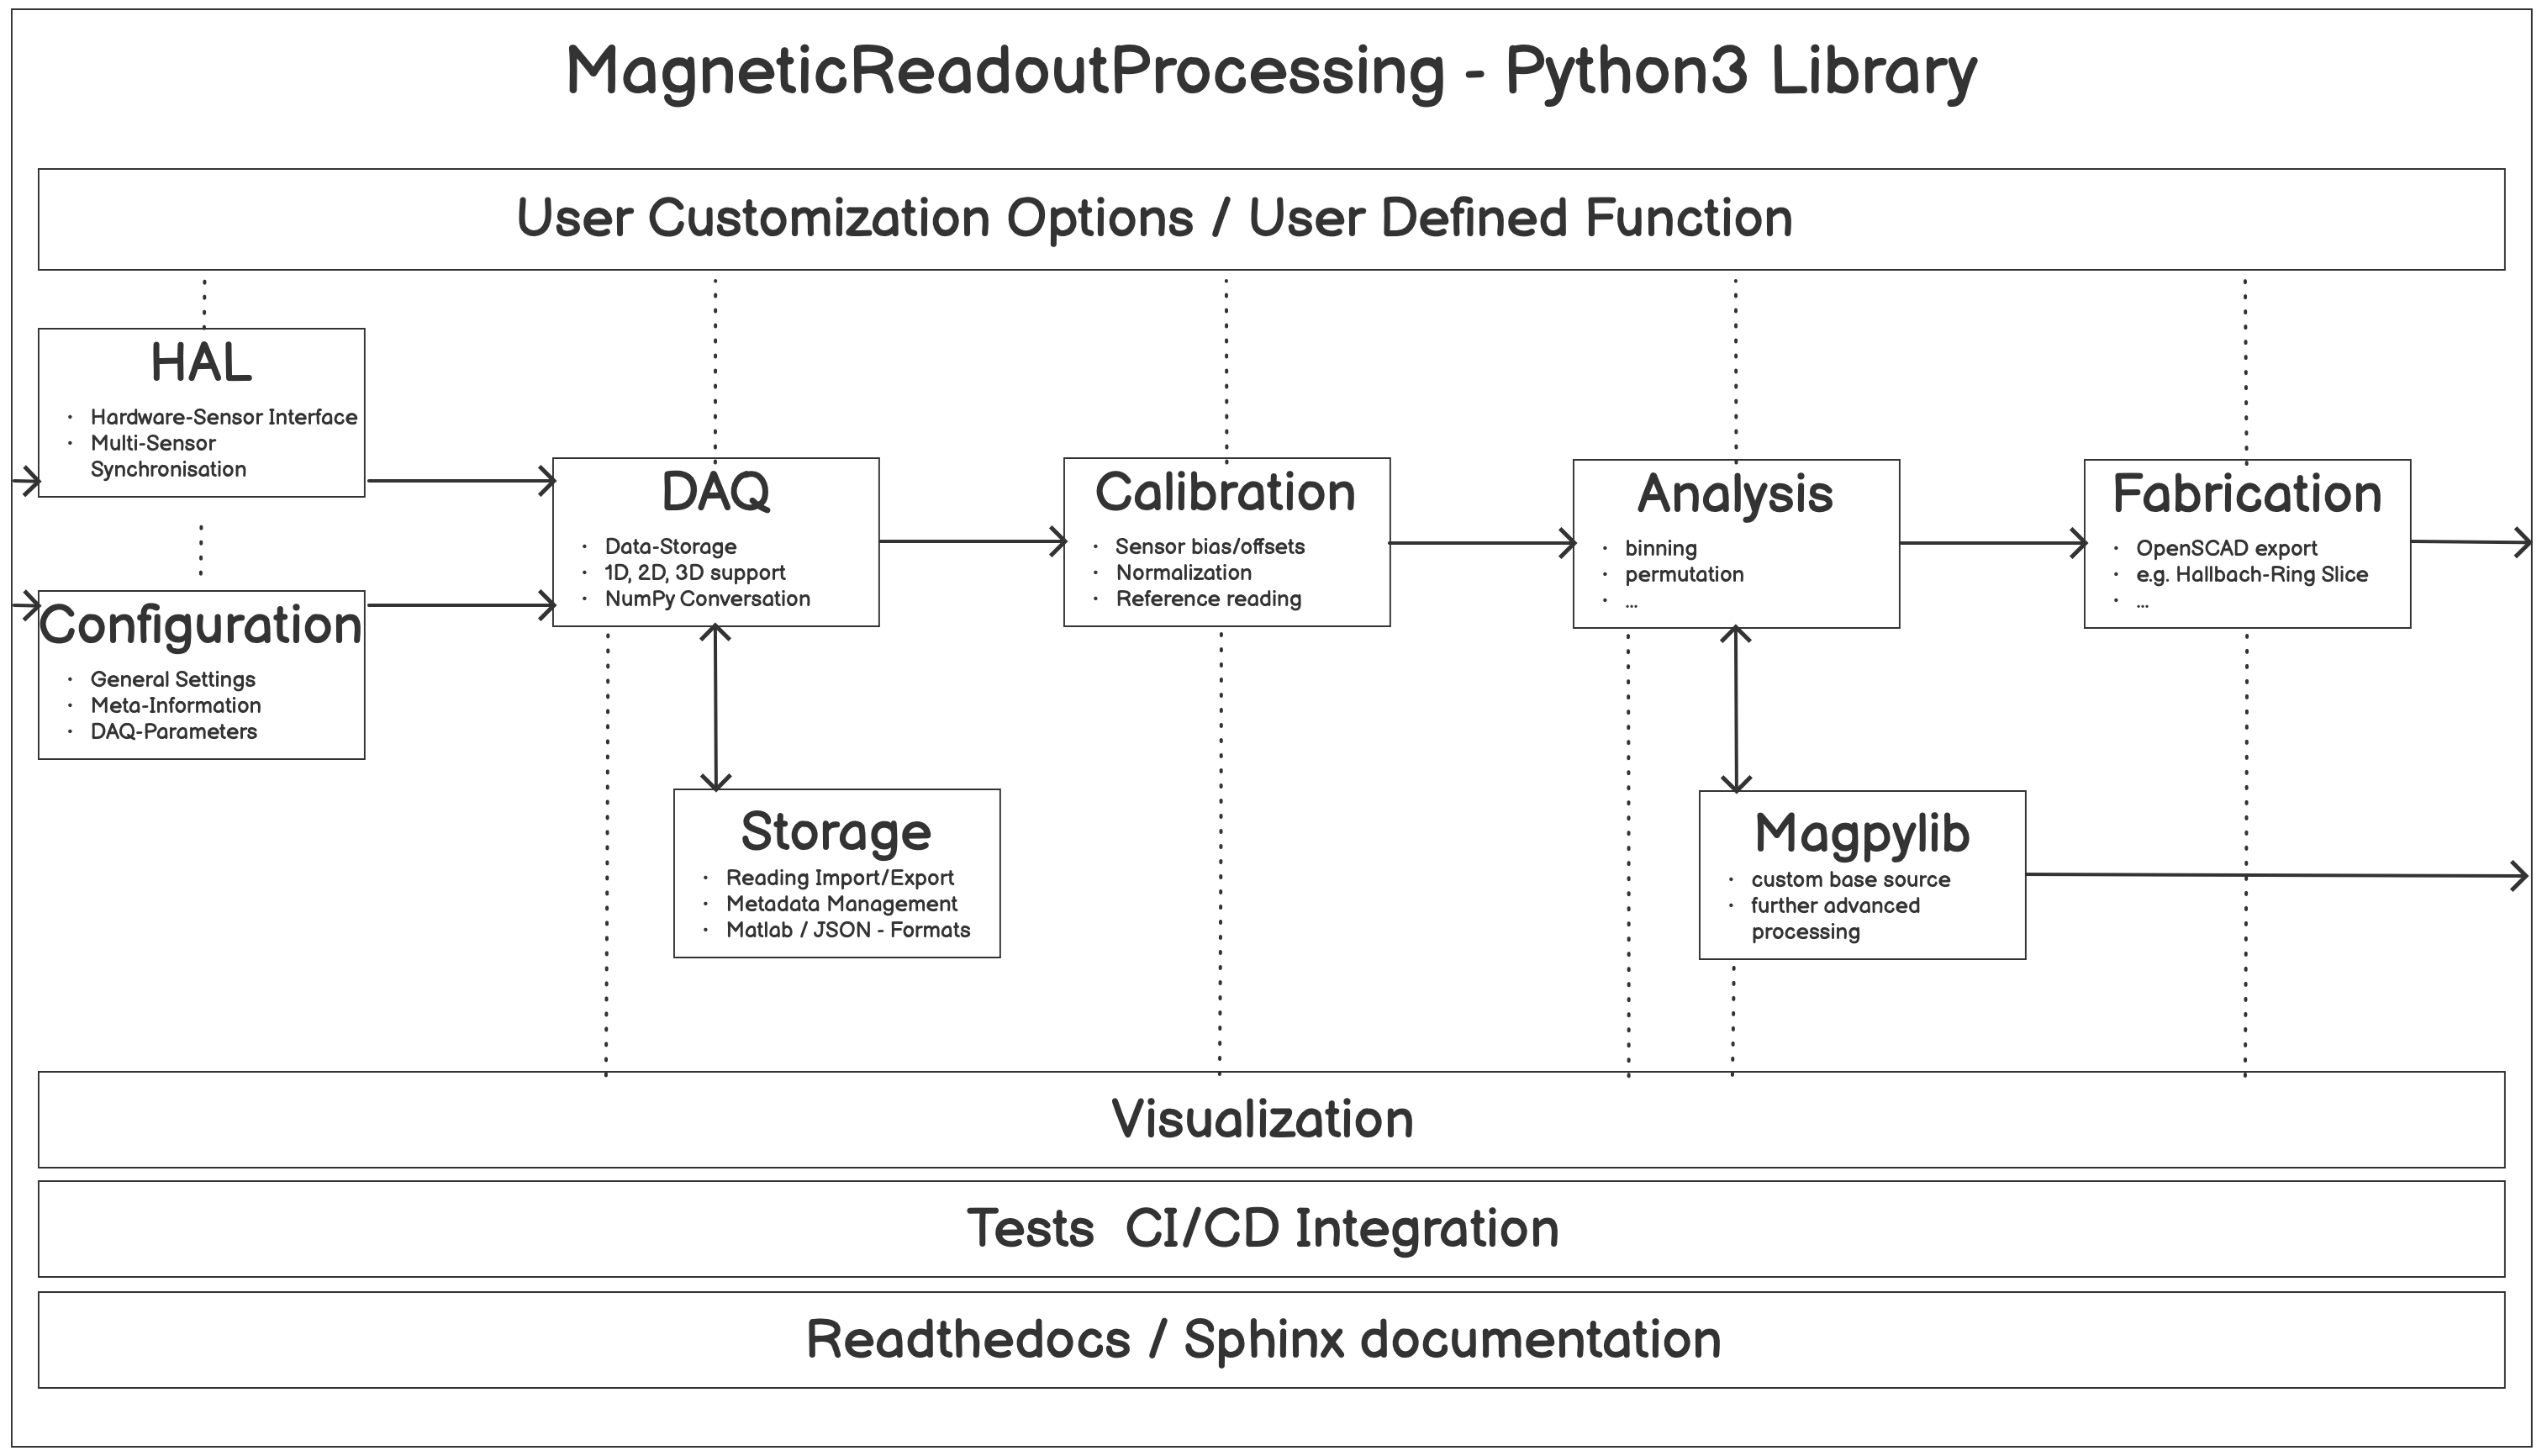
\includegraphics{./generated_images/border_MRP_library_module_high_level_overview.png}
\caption{MRP library module high level overview
\label{MRP_library_module_high_level_overview.png}}
\end{figure}

\hypertarget{user-interaction-points-example}{%
\subsection{User Interaction Points
Example}\label{user-interaction-points-example}}

The following example shows the advantages of using the
\passthrough{\lstinline!User interaction points!}:

A project called \passthrough{\lstinline!HalbachOptimisation!}
\cite{HalbachOptimisation} implements a data analysis step and
optimizes a magnetic field that is as homogeneous as possible within a
circular section using given mechanical dimensions as input parameters
of the magnets used. For this purpose, a mutation of the magnet
positions and rotations is performed. The result is a list of positions
for each magnet.

The \passthrough{\lstinline!HalbachMRIDesigner!}
\cite{HalbachMRIDesigner} opensource project, can generate basic
\gls{cad} drawings for \gls{mri} magnets in a Hallbach configuration. To
do this, the number of magnets and additional parameters for the
properties of the \gls{cad} model to be created are passed to the
function provided as input parameters using a \gls{json} file. The
result is an \passthrough{\lstinline!OpenSCAD!} \cite{OpenSCAD}
based 3D model of the magnet holder.

As a result, there are two projects which are both suitable for the task
of optimizing and creating Hallbach magnets for \gls{mri} applications.
The data structures are not compatible with each other. However, they
are executed manually one after the other to obtain a final result with
manual data conversation.

The library created is intended to solve one problem by providing
standardized and flexible data structures for use with this form of
magnetic field data. By separating the processing pipeline into defined
sub-steps, it should be possible to make individual modules and as a
result functionalities interchangeable by the user.

The implementation of the same functionalities looks as follows after
using the library:

\begin{enumerate}
\def\labelenumi{\arabic{enumi}.}
\tightlist
\item
  \textbf{Create a static set of magnets}
\end{enumerate}

The input parameters of the
\passthrough{\lstinline!HalbachOptimisation!}
\cite{HalbachOptimisation} project are on the one hand the
mechanical dimensions and the number of magnets to be used. We assume
ideal magnets here. However, it should also be possible to import field
data in a more measured form later on. Using the DataAquisition
sub-step, it is possible to generate any number of ideal magnets.

\begin{enumerate}
\def\labelenumi{\arabic{enumi}.}
\setcounter{enumi}{1}
\tightlist
\item
  \textbf{Add custom analysis processing step}
\end{enumerate}

Next, the user creates his own analysis step in order to be able to call
up its functions. In the case of the
\passthrough{\lstinline!HalbachOptimisation!}
\cite{HalbachOptimisation} project, the function signature of the
start function must be changed. This receives the result of the previous
step, in this case the generated magnet data. By optionally setting meta
data in the universal library data type, constants can be replaced in
the analysis function and made dynamically configurable. The return
result also corresponds to this data type so that subsequent steps are
compatible and contains the magnet data with modified position and
rotation data.

\begin{enumerate}
\def\labelenumi{\arabic{enumi}.}
\setcounter{enumi}{2}
\tightlist
\item
  \textbf{Generate fabrication data}
\end{enumerate}

The last step is to call up the
\passthrough{\lstinline!HalbachMRIDesigner!}
\cite{HalbachMRIDesigner} project, which creates the \gls{cad} model
of the magnet holder. The data can also be exported as files here. To
make the project compatible, the function signatures are also adapted
here. In this case, more changes are required, as the configuration file
is loaded from the file system. This logic must be removed in order to
use the added meta data in the input parameter instead.

After these customisation steps, it is possible to execute both projects
one after the other and all required configuration parameters are
contained in the data structure looped through the individual steps as
meta data. This also maps the functionality of a project file, which can
be executed or passed on repeatedly.

This also fulfills the goal of making individual user-created algorithms
interchangeable. If the user now wishes to use a different \gls{cad}
algorithm instead of the \passthrough{\lstinline!HalbachMRIDesigner!}
\cite{HalbachMRIDesigner}, the other steps can simply be preserved
and only the new step needs to be implemented.

\hypertarget{modules}{%
\section{Modules}\label{modules}}

In order to realise the concept of user interaction points, the library
was divided into different modules. These modules can be divided into
two main categories:

\begin{itemize}
\tightlist
\item
  Core - All modules related to measurement data management
\item
  Extensions - Contains modules for visualisations, hardware sensor
  access
\end{itemize}

In each of these categories there are then several sub-categories
divided into User Interaction Points. An overview of these is given in
the subchapters as the following. There are also introductory examples
which provide an overview of the basic functions in the
\passthrough{\lstinline!Examples!} \ref{examples} section, as well as
further examples in the online documentation
\cite{MagneticReadoutProcessingReadTheDocs}.

\hypertarget{core-modules}{%
\subsection{Core Modules}\label{core-modules}}

The included core modules are essential for using the library. Basic
data types are implemented, as well as functions for import and export.
In addition, there are other support scripts that are required
internally.

The following modules are implemented in detail:

\begin{itemize}
\tightlist
\item
  \passthrough{\lstinline!MRPReading!} - storage of measured values
\item
  \passthrough{\lstinline!MRPMeasurementConfig!} - storage of the
  measurement parameters
\item
  \passthrough{\lstinline!MRPMagnetTypes!} - various physical constants
  for basic magnet types
\end{itemize}

The \passthrough{\lstinline!MRPReading!} module performs a crucial role
in streamlining the centralized management of measurement data. It
serves as a storage provider for various measurements, offering
functionalities that facilitate the creation and addition of data
records. To customize and add meta-data, users have the flexibility to
configure parameters through the dedicated
\passthrough{\lstinline!MRPMeasurementConfig!} module into an
\passthrough{\lstinline!MRPReading!} instance.

Within the realm of measurement data, a diverse range of data points can
be seamlessly incorporated. The process is initiated by employing
specialized functions designed for the creation and addition of data
records.

To configure parameters, ensuring a tailored approach to the entire
measurement process, these parameters act as a crucial bridge between
user preferences and the robust capabilities of the
\passthrough{\lstinline!MRPReading!} module.

The system is also designed to be compatible with
\passthrough{\lstinline!Extension Modules!} \ref{extension-modules},
allowing the generation of measurement data through various modules.
This extensibility enhances the versatility of the system, accommodating
diverse measurement scenarios and expanding its utility across different
domains.

To enhance the accessibility and interpretability of the recorded data,
a dedicated module, \passthrough{\lstinline!MRPMagnetTypes!}, comes into
play. This module is specifically designed for the storage of physical
parameters pertaining to the magnets targeted for measurement.

By centralizing this information, users can streamline the subsequent
phases of evaluation and analysis, simplifying the overall process and
ensuring a more efficient and insightful exploration of the collected
data.

At the end of processing, the collected and modified data are typically
exported; various functions are provided for this purpose. This process
is described in the following subchapter.

\hypertarget{storage-and-datamanagement}{%
\subsection{Storage and
Datamanagement}\label{storage-and-datamanagement}}

An important aspect is data import and export. On the one hand, this
allows the library to reuse and archive the measurements. On the other
hand, the focus during development was that it is also possible to use
the data in other programs.

For this purpose, an open, documented export format must be selected.
Ideally, this should be human-readable and viewable with a simple text
editor. This eliminates all binary-based formats such as the Python
pickle built into Python.

Taking these points into account, the \gls{json} format was chosen. This
is human and machine readable and there is a compatible parser for
almost every programming language.

The following code snippet \ref{lst:json_export_format_example} shows
the \gls{json} structure which is generated when a measurement thatt
using the library is exported. Here you can see that by using the
\gls{json} format, all measurement points and metadata are available in
readable plain text.

This means that they can also be read out in other programs. Using
serialization, the \passthrough{\lstinline!MRPReading!} class inherited
from Python-\passthrough{\lstinline!Object!} class is serialized via an
dictionary conversion step. This \gls{json} string can then be processed
directly or written to the file system as a file.

\begin{lstlisting}[caption={JSON export structure of an MRPReading based measurement}, label=lst:json_export_format_example]
{
  "time_start": "Wed Sep 20 08:50:13 2023",
  "time_end": "Wed Sep 20 08:54:13 2023",
  "additional_data": {
      "sensor_device_path": "/dev/ttyUnifiedSensorSingle",
      "sensor_name": "Unified Sensor Single Sensor",
      "sensor_id": "386731533439",
      "sensor_capabilities": ["static", "axis_b", "axis_x", "axis_y", "axis_z", "axis_temp", "axis_stimestamp"],
      "configname": "calibrationtemp30.yaml",
      "runner": "cli"
  },
  "data": [{
      "value": 0.135,
      "is_valid": true,
      "id": 0,
      "temperature": 34.32
  }],
  "measurement_config": {
      "id": "525771256544952",
      "sensor_distance_radius": 40.0,
      "magnet_type": 0
  },
  "name": "calibrationtemp30",
}
\end{lstlisting}

The exported example \ref{lst:json_export_format_example} contains the
following different object keys, which contain the following
information:

\begin{itemize}
\tightlist
\item
  \passthrough{\lstinline!additional\_data!} - Additional user-defined
  metadata
\item
  \passthrough{\lstinline!data!} - Datapoint storage consists of
  measured value, \gls{uuid} and temperature, among other parameters
\item
  \passthrough{\lstinline!measurement\_config!} - Information about the
  sensor used for measurement
\end{itemize}

In addition, further custom objects can be inserted into the \gls{json}
using the functions provided.

Since there are popular data processing frameworks such as
\passthrough{\lstinline!Numpy!} \cite{harris2020array}, or the
program for mathematical calculations, \passthrough{\lstinline!MATLAB!}
are often used, the library also supports export formats for these
systems.

The different formats can be triggered by the user by calling up the
corresponding \passthrough{\lstinline!MRPReading!} class functions:

\begin{itemize}
\tightlist
\item
  \passthrough{\lstinline!.dump()!} - \gls{json}
\item
  \passthrough{\lstinline!.to\_numpy\_matrix()!} -
  \passthrough{\lstinline!Numpy!}-Array of
  \passthrough{\lstinline!data!} object with different options
\item
  \passthrough{\lstinline!.dump\_savemat()!} -
  \passthrough{\lstinline!MATLAB!} mat-file with measurement values and
  temperatures
\end{itemize}

Currently, data re-import of an exported measurement is only supported
via the \gls{json} format, as an export using the other options
(\passthrough{\lstinline!Numpy!}, \passthrough{\lstinline!MATLAB!})loses
data during the export procedure.

\hypertarget{extension-modules}{%
\subsection{Extension Modules}\label{extension-modules}}

The extention modules build on the core modules and offer the user
additional basic functionalities. These include functions for data
acquisition, visualisation and analysis.

\hypertarget{sensor-interface}{%
\subsubsection{Sensor Interface}\label{sensor-interface}}

Another collection of optional modules provided by the library is the
connection of external hardware sensors. All compatible sensors that are
compatible with the firmware developed in the
\passthrough{\lstinline!Unified Sensor!} \ref{unified-sensor} chapter
are supported here. The library provides the following sensor \gls{hal}
modules for this purpose:

\begin{itemize}
\tightlist
\item
  \passthrough{\lstinline!MRPHal!} - Firmware protocol implementation
\item
  \passthrough{\lstinline!MRPHalLocal!} - \gls{usb} sensor interface
\item
  \passthrough{\lstinline!MRPHalRemote!} - Remote sensor interface
\end{itemize}

These provide functions to communicate with a connected hardware sensor
and send commands to it. To generate these and convert the received
measurement data into the appropriate format for the core modules, there
is a suitable module for each sensor type:

\begin{itemize}
\tightlist
\item
  \passthrough{\lstinline!MRPReadingSourceStatic!} - for 1D and 2D
  sensors such as \passthrough{\lstinline!1D: Single Sensor!}
  \ref{d-single-sensor}
\item
  \passthrough{\lstinline!MRPReadingSourceFullsphere!} - for 3D sensors
  such as \passthrough{\lstinline!3D: Fullsphere!} \ref{d-fullsphere}
\end{itemize}

The decision which of these modules to use is made automatically
depending on the connected hardware. For this purpose, a static function
\passthrough{\lstinline!createReadingSourceInstance!} is implemented in
the base class \passthrough{\lstinline!MRPReadingSource!}, which
automatically creates the appropriate instance based on the sensor
capabilites.

\hypertarget{visualisation}{%
\subsubsection{Visualisation}\label{visualisation}}

In order to give the user the possibility to display the recorded data
visually, two modules were created, which can graphically prepare
\passthrough{\lstinline!MRPReading!} instances:

\begin{itemize}
\tightlist
\item
  \passthrough{\lstinline!MRPVisualization!} - different table and graph
  based plots
\item
  \passthrough{\lstinline!MRPPolarVisualization!} - fullsphere map plots
\end{itemize}

On the one hand, it is possible with the
\passthrough{\lstinline!MRPVisualization!} module to display measurement
data as a table or plot (e.g.~stream, line, point). This makes it
possible, for example, to visually identify outliers or trends in the
measurement data. These can also be saved as an image file. The module
is compatible with all measurement data.

In contrast to the \passthrough{\lstinline!MRPPolarVisualization!}
module, this provides functions to create 2D map plots a polar
coordinate system. This requires measurement data with additionally set
spatial coordinates. These can be generated automatically with the
\passthrough{\lstinline!3D: Fullsphere!} \ref{d-fullsphere} sensor, or
the user must provide the spatial information from another source.

\hypertarget{analysis}{%
\subsubsection{Analysis}\label{analysis}}

Data analysis offers the user the greatest flexibility to implement
their own modules. For this reason \passthrough{\lstinline!MRPAnalysis!}
contains functions for calculating the following data analyses, which
are compatible with class instances of
\passthrough{\lstinline!MRPReading!}:

\begin{itemize}
\tightlist
\item
  \passthrough{\lstinline!std\_deviation!} - Standard deviation
\item
  \passthrough{\lstinline!mean!} - Mean value
\item
  \passthrough{\lstinline!variance!} - Variance
\item
  \passthrough{\lstinline!CoG!} - Center of gravity
\item
  \passthrough{\lstinline!binning!} - Distribution of a sample by means
  of a histogram
\item
  \passthrough{\lstinline!k-nearest!} - K-nearest neighbors
\end{itemize}

In addition, the export function
\passthrough{\lstinline!.to\_numpy\_matrix!} enables further processing
of the data in the \passthrough{\lstinline!Numpy!}
\cite{harris2020array} framework, in which many other standard
analysis functions are implemented.

\hypertarget{multi-sensor-setup}{%
\section{Multi Sensor Setup}\label{multi-sensor-setup}}

At the current described scenarios, it is only possible to detect and
use sensors that are directly connected to the host \gls{pc}. It has the
disadvantage that there must always be a physical connection. This can
make it difficult to install multiple sensors in measurement setups
where space or cable routing options are limited.

Multibe sensor can be connected to any \gls{pc} which is available on
the network. This can be a \gls{sbc} (e.g.~a Raspberry Pi). The small
footprint and low power consumption make it a good choice. It can also
be used in a temperature chamber.

The \passthrough{\lstinline!MRPProxy!} \ref{MRPlib_Proxy_Module.png}
module has been developed to allow forwarding and interaction with
several sensors over a network connection using a \gls{rest} interface.

The approach of implementing this via a \gls{rest} interface also offers
the advantage that several measurements or experiments can be recorded
at the same time with one remote sensor setup.

\begin{figure}
\centering
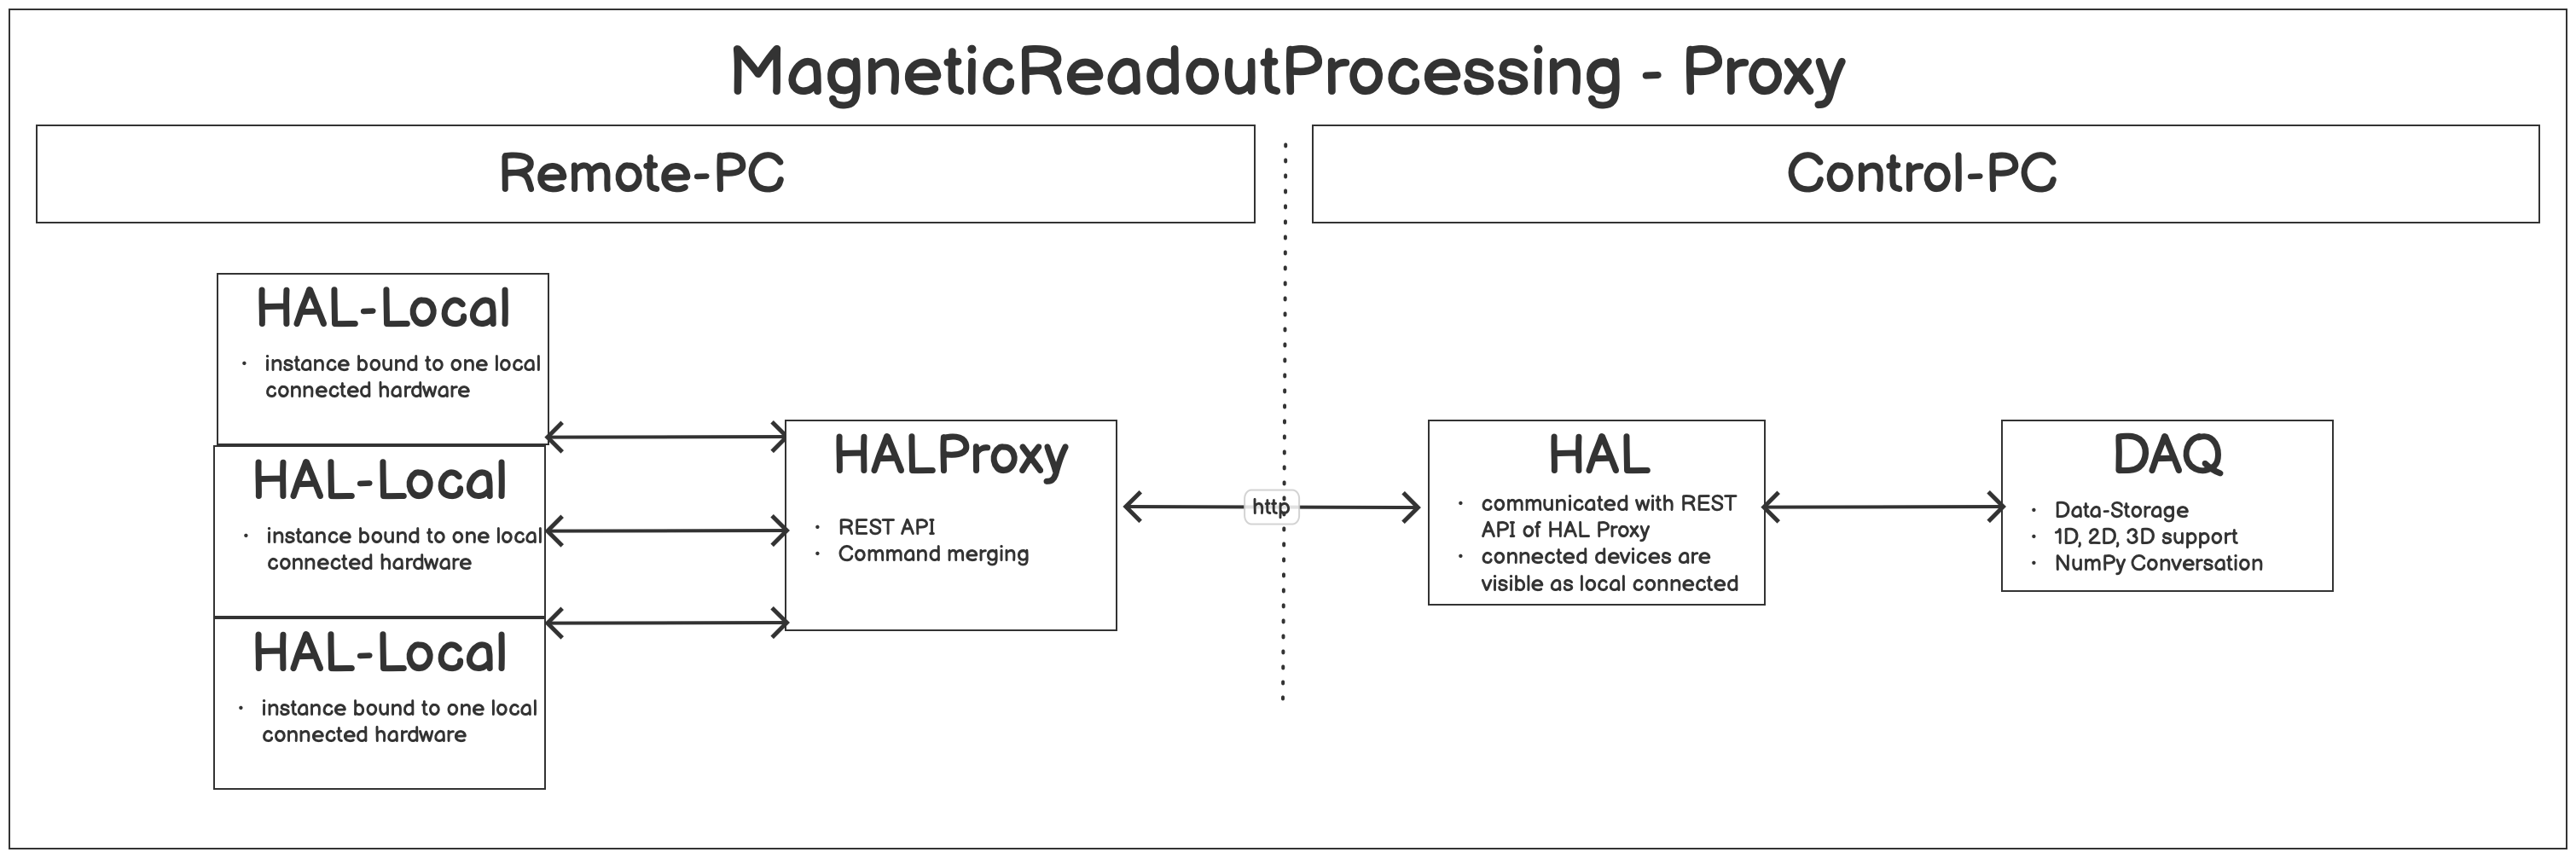
\includegraphics{./generated_images/border_MRPlib_Proxy_Module.png}
\caption{MRPlib Proxy Module \label{MRPlib_Proxy_Module.png}}
\end{figure}

Another application example is when sensors are physically separated or
there are long distances between them. By connecting several sensors via
the proxy module, it is possible to link several instances and all
sensors available in the network are available to the
\passthrough{\lstinline!control!} \gls{pc}.

\begin{figure}
\centering
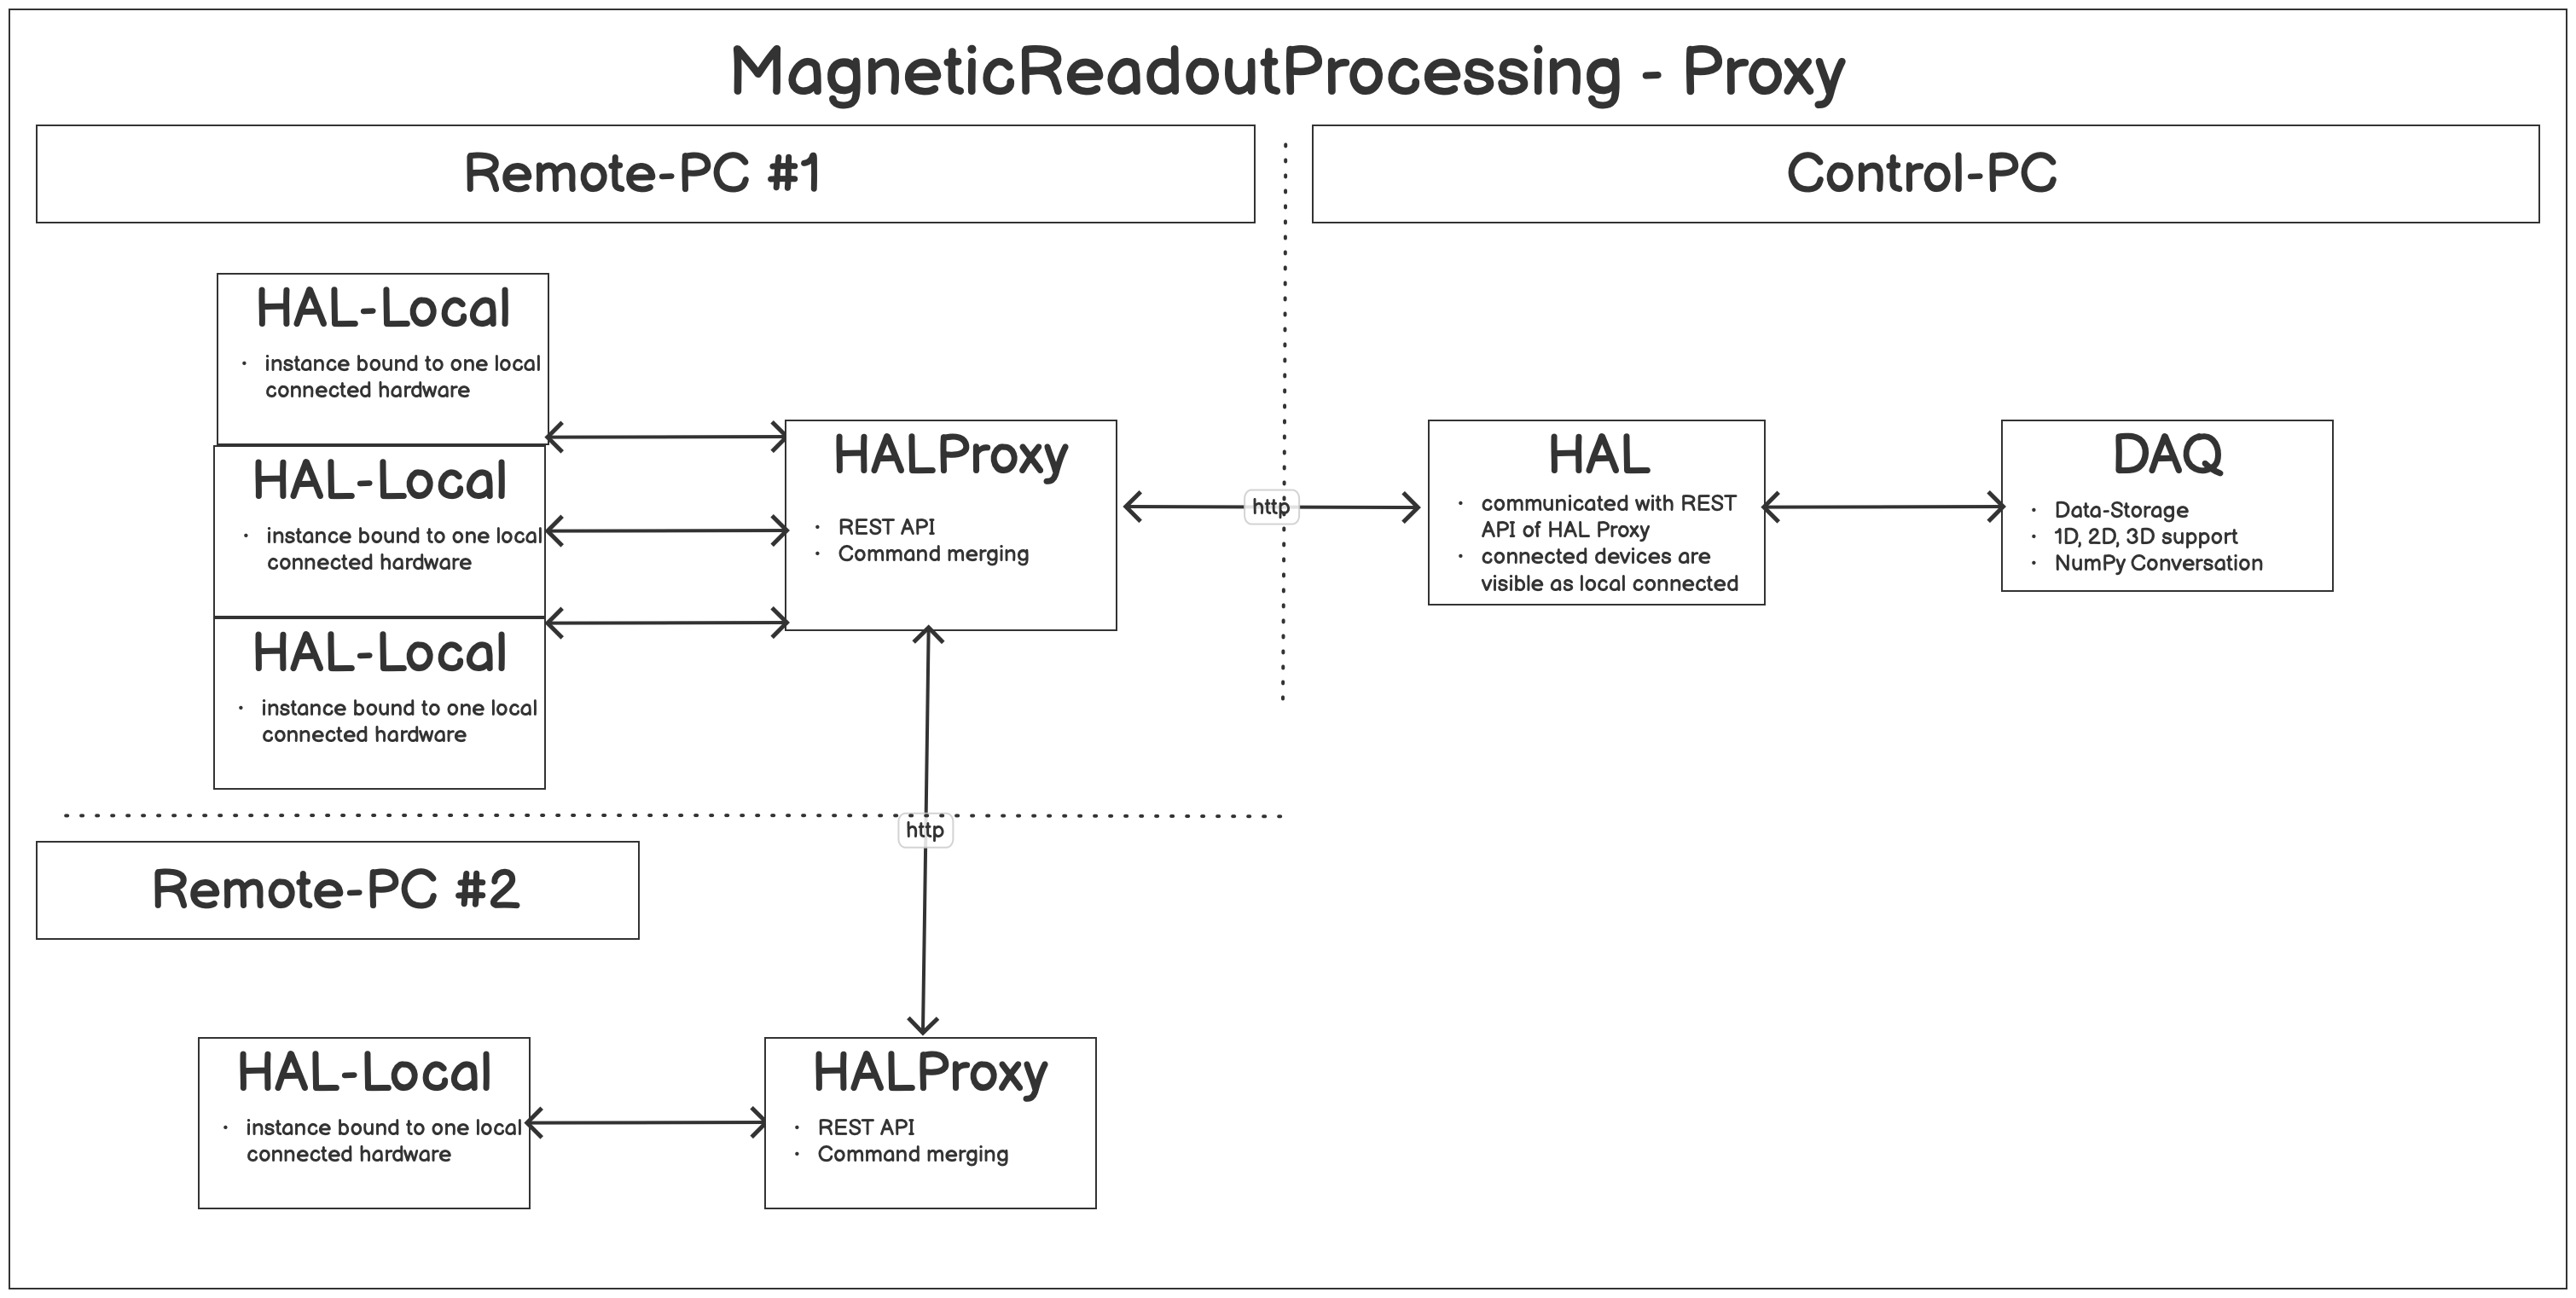
\includegraphics{./generated_images/border_Example_MRP_proxy_module_usage,_using_two_remote_(+pc)s.png}
\caption{Example MRP proxy module usage, using two remote \gls{pc}s
\label{Example_MRP_proxy_module_usage,_using_two_remote_(+pc)s.png}}
\end{figure}

The figure
\ref{Example_MRP_proxy_module_usage,_using_two_remote_(+pc)s.png} shows
the modified \passthrough{\lstinline!multi-proxy - multi-sensor!}
topology. Here, both proxy instances do not communicate directly with
the \passthrough{\lstinline!control!} \gls{pc}, but the proxy instance
\passthrough{\lstinline!remote!}\gls{pc} \passthrough{\lstinline!\#2!}
can acces the proxy running on \passthrough{\lstinline!remote!}\gls{pc}
\passthrough{\lstinline!\#1!}.

The \passthrough{\lstinline!control!} \gls{pc} only communicates with
the \passthrough{\lstinline!remote!} \gls{pc}
\passthrough{\lstinline!\#1!}, but can access all sensors in this chain.

\hypertarget{network-proxy}{%
\subsection{Network-Proxy}\label{network-proxy}}

The figure \ref{MRPlib_Proxy_Module.png} shows the separation of the
various \gls{hal} instances, which communicate with the physically
connected sensors on the \passthrough{\lstinline!remote!} \gls{pc} and
the \passthrough{\lstinline!control!} \gls{pc} side, which communicates
with the remote side via the network. For the user, nothing changes in
the procedure for setting up a measurement. The
\passthrough{\lstinline!MRPProxy!} \gls{cli} application must always be
started \ref{lst:mrpcli_proxy_start} on the \gls{pc} with connected
hardware sensors attached.

\begin{lstlisting}[language=bash, caption={MRPproxy usage to enable local sensor usage over network}, label=lst:mrpcli_proxy_start]
# START PROXY INSTNACE WITH TWO LOCALLY CONNECTED SENSORS
$ python3 mrpproxy.py proxy launch /dev/ttySENSOR_A /dev/ttySENSOR_B # add another proxy instance http://proxyinstance_2.local for multi-sensor, multi-proxy chain
Proxy started. http://remotepc.local:5556/
PRECHECK: SENSOR_HAL: 1337 # SENSOR A FOUND
PRECHECK: SENSOR_HAL: 4242 # SENSOR B FOUND
Terminate  Proxy instance [y/N] [n]: 
\end{lstlisting}

After the proxy instance has been successfully started, it is optionally
possible to check the status via the \gls{rest} interface:
\ref{lst:mrpcli_config_rest}

\begin{lstlisting}[language=bash, caption={MRPProxy REST endpoint query examples}, label=lst:mrpcli_config_rest]
# GET PROXY STATUS
$ wget http://proxyinstance.local:5556/proxy/status
{
"capabilities":[
  "static",
  "axis_b",
  "axis_x",
  "axis_y",
  "axis_z",
  "axis_temp",
  "axis_stimestamp"
],
"commands":[
  "status",
  "initialize",
  "disconnect",
  "combinedsensorcnt",
  "sensorcnt",
  "readsensor",
  "temp"
]}
# RUN A SENSOR COMMAND AND GET THE TOTAL SENSOR COUNT
$ wget http://proxyinstance.local:5556/proxy/command?cmd=combinedsensorcnt
{
"output":[
  "2"
]}
\end{lstlisting}

The query result shows that the sensors are connected correctly and that
their capabilites have also been recognised correctly. To be able to
configure a measurement on the \passthrough{\lstinline!control!}
\gls{pc}, only the \gls{ip} address or hostname of the \gls{pc} running
an \passthrough{\lstinline!MRPProxy!} instance is required
\ref{lst:mrpcli_config_using_rpc}.

\begin{lstlisting}[language=bash, caption={MRPcli usage example to connect with a network sensor}, label=lst:mrpcli_config_using_rpc]
# CONFIGURE MEASUREMENT JOB USING A PROXY INSTANCE
$ MRPcli config setupsensor testcfg --path http://proxyinstance.local:5556
> remote sensor connected: True using proxy connection:
> http://proxyinstance.local:5556 with 1 local sensor connected
\end{lstlisting}

\hypertarget{sensor-syncronisation}{%
\subsection{Sensor Syncronisation}\label{sensor-syncronisation}}

Another important aspect when using several sensors via the proxy system
is the synchronisation of the measurement intervals between the sensors.
Individual sensor setups do not require any additional synchronisation
information, as this is communicated via the \gls{usb} interface.

If several sensors are connected locally, they can be connected to each
other via their sync input using short cables. One sensor acts as the
central clock as described in \ref{sensor-syncronisation-interface}.
this no longer works for long distances and the syncronisation must be
made via a shared network connection.

If time-critical synchronisation over the network is required, \gls{ptp}
and \gls{pps} output functionality \cite{PTPIEEE1588} can be used on
many \gls{sbc}, such as the
\passthrough{\lstinline!Raspberry-Pi Compute Module!}.

\hypertarget{command-router}{%
\subsection{Command-Router}\label{command-router}}

As it is possible to connect many identical sensors to one host, it must
be possible to address them separately. This separation is done by the
\passthrough{\lstinline!MRPProxy!} module and is a separate part from
the core \gls{mrp}-library, to keep installation package dependencies
small.

Each connected sensor is accessed via the text-based \gls{cli}, this is
initially the same for each sensor. The only identification feature is
the sensor \gls{uuid} by using the \passthrough{\lstinline!id!} command
of the sensor \gls{cli}.

The \passthrough{\lstinline!MRPProxy!} instance claims to be a sensor to
the host \gls{pc} running \gls{mrp} \gls{cli}, so the multiple sensors
must be combined into one virtual one. This is done in several steps,
start procedure described by the following sub-chapters.

\hypertarget{construct-the-sensor-id-lookup-table}{%
\subsubsection{Construct the Sensor ID
LookUp-Table}\label{construct-the-sensor-id-lookup-table}}

Immediately after starting the \passthrough{\lstinline!MRPProxy!}, the
\gls{uuid}s of all locally connected sensors are read out. These are
stored together with the class instance of the
\passthrough{\lstinline!MRPHal!} module in a \gls{lut}. This makes it
possible to address a sensor directly using its \gls{uuid}.

\hypertarget{merging-the-sensor-capabilities}{%
\subsubsection{Merging the Sensor
Capabilities}\label{merging-the-sensor-capabilities}}

\begin{longtable}[]{@{}llll@{}}
\caption{Sensor capabilities merging algorithm
\label{Sensor_capabilities_merging_algorithm.csv}}\tabularnewline
\toprule
SENSOR A & SENSOR B & MERGED CAPABILITIES & CAPABLE SENSORS ID
LUT\tabularnewline
\midrule
\endfirsthead
\toprule
SENSOR A & SENSOR B & MERGED CAPABILITIES & CAPABLE SENSORS ID
LUT\tabularnewline
\midrule
\endhead
static & & static & A\tabularnewline
& dynamic & dynamic & B\tabularnewline
axis\_temp & axis\_temp & axis\_temp & A B\tabularnewline
axis\_x & axis\_x & axis\_x & A B\tabularnewline
\bottomrule
\end{longtable}

When using sensors with different capabilites, these must be combined.
These are used to select the appropriate measurement mode for a
measurement. For this purpose, the \passthrough{\lstinline!info!}
command of each sensor is queried. This information is added to the
previously created \gls{lut}. Duplicate entries are summarised (see
Table \ref{Sensor_capabilities_merging_algorithm.csv}) and returned to
the host when the \passthrough{\lstinline!info!} \ref{lst:mtsc} command
is received over network.

\begin{lstlisting}[language=bash, caption={MRPproxy REST enpoiint query examples}, label=lst:mtsc]
# QUERY Network-Proxy capabilities
$ wget http://proxyinstance.local:5556/proxy/status
{"capabilities":[
"static",
"dynamic",
"axis_temp",
"axis_x"
]}
\end{lstlisting}

The same procedure is performed for the
\passthrough{\lstinline!commands!} \gls{cli}-command of each sensor, to
merge available commands of connected sensors into the \gls{lut}.

\hypertarget{dynamic-extension-of-the-available-network-proxy-commands}{%
\subsubsection{Dynamic extension of the available Network-Proxy
Commands}\label{dynamic-extension-of-the-available-network-proxy-commands}}

In order for the host to be able to send a command to the network
multi-sensor setup, the command received must be forwarded to the
correct sensor. In addition, there are commands such as the previously
used \passthrough{\lstinline!info!} or \passthrough{\lstinline!status!}
command, which must be intercepted by the
\passthrough{\lstinline!MRPProxy!} module so that it can be handled
differently (see example \ref{lst:mtsc}).

To realize this, a \gls{lut} was created in the previous steps, which
contains information regarding
\passthrough{\lstinline!requested capability!} -\textgreater{}
\passthrough{\lstinline!sensor!}-\gls{uuid} -\textgreater{}
\passthrough{\lstinline!physical sensor!} and allows the commands to be
routed.

For commands where there are several entries for
\passthrough{\lstinline!CAPABLE SENSORS ID LUT!}
\ref{Sensor_capabilities_merging_algorithm.csv}, there are two possible
approaches to how the command is processed:

\begin{itemize}
\tightlist
\item
  Redirect to each capable sensor
\item
  Extend commands using an id parameter
\end{itemize}

These two methods have been implemented and are applied automatically.
The decision is based on which hardware sensors are connected. In a
setup where only the same sensor variants are connected,
\passthrough{\lstinline!redirect to each capable sensor!} is applied.
This offers a time advantage as fewer commands need to be sent from the
host. Thus, with a \passthrough{\lstinline!readsensor!} command, all
sensors are read out via one command and the summarized result is
transmitted to the host.

The \passthrough{\lstinline!extend commands using an id parameter!}
strategy is used for different sensors. Each command is extended on the
\passthrough{\lstinline!Network-Proxy!} \ref{network-proxy} by another
\gls{uuid} parameter, according to the following scheme:

\begin{itemize}
\tightlist
\item
  \passthrough{\lstinline!readsensor <axis> <sensor number>!}
  -\textgreater{} \passthrough{\lstinline!readsensor <axis> <ID>!}
\item
  \passthrough{\lstinline!opmode!}-\textgreater{}
  \passthrough{\lstinline!opmode <ID>!}
\end{itemize}

This allows the host to address individual sensors directly via their
specific \gls{uuid}.

\hypertarget{examples}{%
\section{Examples}\label{examples}}

The following shows some examples of how the \gls{mrp}-library can be
used. These examples are limited to a functional minimum for selected
modules of the \gls{mrp}-library. The documentation \ref{documentation}
contains further and more detailed examples. Many basic examples are
also supplied in the form of the test scripts used for testing
\ref{testing}.

\hypertarget{mrpreading}{%
\subsection{MRPReading}\label{mrpreading}}

The \passthrough{\lstinline!MRPReading!} is the key module of the
\gls{mrp} core. It is used to manage the measurement data and can be
imported and exported. The following example
\ref{lst:mrpexample_reading} shows how a measurement is created and
measurement points are added in the form of
\passthrough{\lstinline!MRPReadingEntry!} instances.

An important point is the management of the meta data, which further
describes the measurement. This is realised in the example using the
\passthrough{\lstinline!set\_additional\_data!} function.

\begin{lstlisting}[language=Python, caption={MRPReading example for setting up an basic measurement}, label=lst:mrpexample_reading]
from MRP import MRPReading, MRPMeasurementConfig
# [OPTIONAL] CONFIGURE READING USING MEASUREMENT CONFIG INSTANCE
config: MRPMeasurementConfig = MRPMeasurementConfig
config.sensor_distance_radius(40) # 40mm DISTANCE BETWEEN MAGNET AND SENSOR
config.magnet_type(N45_CUBIC_12x12x12) # CHECK MRPMagnetTypes.py FOR IMPLEMENTED TYPES
# CREATE READING
reading: MRPReading = MRPReading(config)
# ADD METADATA
reading.set_name("example reading")
## ADD FURTHER DETAILS
reading.set_additional_data("description", "abc")
reading.set_additional_data("test-number", 1)
# INSERT A DATAPOINT
measurement = MRPReadingEntry.MRPReadingEntry()
measurement.value = random.random()
reading.insert_reading_instance(measurement, False)
# USE MEASURED VALUES IN OTHER FRAMEWORKS / DATAFORMATS
## NUMPY
npmatrix: np.ndarray = reading.to_numpy_matrix()
## CSV
csv: []= reading.to_value_array()
## JSON
js: dict= reading.dump()
# EXPORT READING TO FILE
reading.dump_to_file("exported_reading.mag.json")
# IMPORT READING
imported_reading: MRPReading = MRPReading()
imported_reading.load_from_file("exported_reading.mag.json")
\end{lstlisting}

Finally, the measurement is exported for archiving and further
processing; various export formats are available. Using the
\passthrough{\lstinline!dump\_to\_file!} function, the measurement can
be converted into an open \gls{json} format. This file can then be
imported again using the \passthrough{\lstinline!load\_from\_file!}
function.

\hypertarget{mrphal}{%
\subsection{MRPHal}\label{mrphal}}

After generating simple measurements with random values in the previous
example \ref{mrpreading}, the next step is to record real sensor data.
For this purpose, the \passthrough{\lstinline!MRPHal!} module was
developed, which can interact with all
\passthrough{\lstinline!Unified Sensor!} \ref{unified-sensor}-compatible
sensors. In the following example \ref{lst:mrpexample_hal}, an
\passthrough{\lstinline!1D: Single Sensor!} \ref{d-single-sensor} is
connected locally to the host \gls{pc}.

\begin{lstlisting}[language=Python, caption={MRPHal example to use an connected hardware sensor to store readings inside of a measurement}, label=lst:mrpexample_hal]
from MRP import MRPHalSerialPortInformation, MRPHal, MRPBaseSensor, MRPReadingSource
# SEARCH FOR CONNECTED SENSORS
## LISTS LOCAL CONNECTED OR NETWORK SENSORS
system_ports = MRPHalSerialPortInformation.list_sensors()
sensor = MRPHal(system_ports[0])
# OR USE SPECIFIED SENSOR DEVICE
device_path = MRPHalSerialPortInformation("UNFSensor1")
sensor = MRPHal(device_path)
# RAW SENSOR INTERACTION MODE
sensor.connect()
basesensor = MRPBaseSensor.MRPBaseSensor(sensor)
basesensor.query_readout()
print(basesensor.get_b()) # GET RAW MEASUREMENT
print(basesensor.get_b(1)) # GET RAW DATA FROM SENSOR WITH ID 1
# TO GENERATE A READING THE perform_measurement FUNCTION CAN BE USED
reading_source = MRPReadingSourceHelper.createReadingSourceInstance(sensor)
result_readings: [MRPReading] = reading_source.perform_measurement(_readings=1, _hwavg=1)
\end{lstlisting}

In general, a sensor can be connected using its specific system path or
the sensor-\gls{uuid} via the
\passthrough{\lstinline!MRPHalSerialPortInformation!} function. Locally
connected or network sensors can also be automatically recognised using
the \passthrough{\lstinline!list\_sensors!} function. Once connected,
these are then converted into a usable data source using the
\passthrough{\lstinline!MRPReadingSource!} module. This automatically
recognises the type of sensor and generated an
\passthrough{\lstinline!MRPReading!} instance with the measured values
of the sensor.

\hypertarget{mrpsimulation}{%
\subsection{MRPSimulation}\label{mrpsimulation}}

If no hardware sensor is available or for the generation of test data,
the \passthrough{\lstinline!MRPSimulation!} module is available. This
contains a series of functions that simulate various magnets and their
fields. The result is a complete \passthrough{\lstinline!MRPReading!}
measurement with a wide range of set meta data.

The example \ref{lst:mrpexample_simulation} illustrated the basic usage.
Different variations of the \passthrough{\lstinline!generate\_reading!}
function offers the user additional parameterisation options, such as
random polarisation direction or a defined centre-of-gravity vector. The
data is generated in the background using the
\passthrough{\lstinline!magpylib!} \cite{ortner2020magpylib} library
according to the specified parameters.

\begin{lstlisting}[language=Python, caption={MRPSimulation example illustrates the usage of several data analysis functions}, label=lst:mrpexample_simulation]
from MRP import MRPSimulation, MRPPolarVisualization, MRPReading
# GENERATE SILUMATED READING USING A SIMULATED HALLSENSOR FROM magpy LIBRARY
reading = MRPSimulation.generate_reading(MagnetType.N45_CUBIC_12x12x12,_add_random_polarisation=True)
# GENERATE A FULLSPHERE MAP READING
reading_fullsphere = MRPSimulation.generate_random_full_sphere_reading()
# RENDER READING TO FILE IN 3D
visu = MRPPolarVisualization(reading)
visu.plot3d(None)
visu.plot3d("simulated_reading.png")
# EXPORT READING
reading.dump_to_file("simulated_reading.mag.json")
\end{lstlisting}

\hypertarget{mrpanalysis}{%
\subsection{MRPAnalysis}\label{mrpanalysis}}

Once data can be acquired using hardware or software sensors, the next
step is to analyse this data. \gls{mrp} provides some simple analysis
functions for this purpose. The code example shows the basic use of the
module. The \passthrough{\lstinline!Evaluation!} \ref{evaluation}
chapter shows how the user can implement their own algorithms and add
them to the library.

\begin{lstlisting}[language=Python, caption={MRPAnalysis example code performs several data analysis steps}, label=lst:mrpexample_analysis]
from MRP import MRPAnalysis, MRPReading
# CREATE A SAMPLE MEASUREMENT WITH SIMULATED DATA
reading = MRPSimulation.generate_reading(MagnetType.N45_CUBIC_10x10x10)
# CALCULATE MEAN
print(MRPAnalysis.calculate_mean(reading))
# CALCULATE STD DEVIATION ON TEMPERATURE AXIS
print(MRPAnalysis.calculate_std_deviation(reading, _temperature_axis=True))
# CALCULATE CENTER OF GRAVITY
(x, y, z) = MRPAnalysis.calculate_center_of_gravity(reading)
# APPLY CALIBRATION READING TO REMOVE BACKGROUND NOISE
calibration_reading = MRPSimulation.generate_reading(MagnetType.N45_CUBIC_10x10x10, _ideal = True)
MRPAnalysis.apply_calibration_data_inplace(calibration_reading, reading)
\end{lstlisting}

\hypertarget{mrpvisualisation}{%
\subsection{MRPVisualisation}\label{mrpvisualisation}}

This final example shows the use of the
\passthrough{\lstinline!MRPVisualisation!} module, which provides
general functions for visualising measurements. The visualisation
optionsmakes it possible to visually assess the results of a
measurement. This is particularly helpful for full-sphere measurements
recorded with the \passthrough{\lstinline!3D: Fullsphere!}
\ref{d-fullsphere} sensor. The sub-module
\passthrough{\lstinline!MRPPolarVisualisation!} is specially designed
for these. The figure
\ref{Example_full_sphere_plot_of_an_measurement_using_the_MRPVisualisation_module.png}
shows a plot of a fullsphere measurement. It is also possible to export
the data from the \passthrough{\lstinline!MRPAnalysis!} module
graphically as diagrams. The \passthrough{\lstinline!MRPVisualisation!}
modules are used here. The following example
\ref{lst:mrpexample_visualisation} shows the usage of both modules.

\begin{lstlisting}[language=Python, caption={MRPVisualisation example which plots a fullsphere to an image file}, label=lst:mrpexample_visualisation]
from MRP import MRPPolarVisualization
# CREATE MRPPolarVisualization INSTANCE
## IT CAN BE REUSED CALLING plot2d AGAIN, AFTER LINKED READING DATA WERE MODIFIED
visu = MRPPolarVisualization.MRPPolarVisualization(reading)
# 2D PLOT INTO A WINDOW
visu.plot2d_top(None)
visu.plot2d_side(None)
# 3D PLOT TO FILE
visu.plot3d(os.path.join('./plot3d_3d.png'))
# PLOT ANALYSIS RESULTS
from MRP import MRPDataVisualization
MRPDataVisualization.MRPDataVisualization.plot_error([reading_a, reading_b, reading_c])
\end{lstlisting}

\begin{figure}
\centering
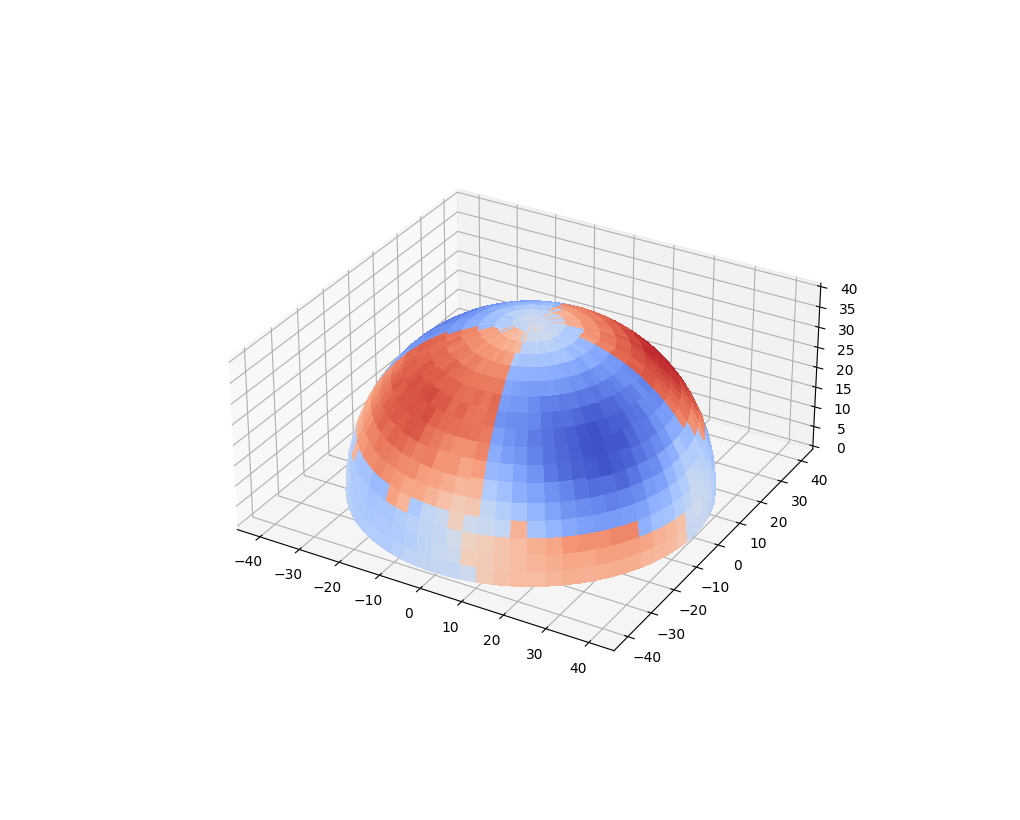
\includegraphics{./generated_images/border_Example_full_sphere_plot_of_an_measurement_using_the_MRPVisualisation_module.png}
\caption{Example full sphere plot of an measurement using the
MRPVisualisation module
\label{Example_full_sphere_plot_of_an_measurement_using_the_MRPVisualisation_module.png}}
\end{figure}

\hypertarget{mrphallbacharraygenerator}{%
\subsection{MRPHallbachArrayGenerator}\label{mrphallbacharraygenerator}}

The following example code \ref{lst:mrpexample_hallbach}, shows how a
simple Hallbach magnetic ring can be generated.

This can then be used to construct a Halbach ring magnet (see chapter
\ref{magnet-system}) for a low-field \gls{mri}.

Eight random measurements are generated here. It is important that the
magnet type (here \passthrough{\lstinline!N45\_CUBIC\_15x15x15!}) is
specified. This is necessary so that the correct magnet cutouts can be
generated when creating the 3D model.

After the measurements have been generated, they are provided with a
position and rotation offset according to the Hallbach design and
calucation scheme \cite{HallbachMagnetDesignPaper} using the
\passthrough{\lstinline!MRPHallbachArrayGenerator!} module.

\begin{lstlisting}[language=Python, caption={MRPHallbachArrayGenerator example for generating an OpenSCAD based hallbach ring}, label=lst:mrpexample_hallbach]
readings = []
for idx in range(8):
  # GENERATE EXAMPLE READINGS USING N45 CUBIC 15x15x15 MAGNETS
  readings.append(MRPSimulation.MRPSimulation.generate_reading(MRPMagnetTypes.MagnetType.N45_CUBIC_15x15x15))
## GENERATE HALLBACH
hallbach_array: MRPHallbachArrayGenerator.MRPHallbachArrayResult = MRPHallbachArrayGenerator.MRPHallbachArrayGenerator.generate_1k_hallbach_using_polarisation_direction(readings)
# EXPORT TO OPENSCAD
## 2D MODE DXF e.g. for lasercutting
MRPHallbachArrayGenerator.MRPHallbachArrayGenerator.generate_openscad_model([hallbach_array], "./2d_test.scad",_2d_object_code=True)
## 3D MODE e.g. for 3D printing
MRPHallbachArrayGenerator.MRPHallbachArrayGenerator.generate_openscad_model([hallbach_array], "./3d_test.scad",_2d_object_code=False)
\end{lstlisting}

In the last step, a 3D model with the dimensions of the magnet type set
is generated from the generated magnet positions. The result is an
\passthrough{\lstinline!OpenSCAD!} \cite{OpenSCAD} file, which
contains the module generated. After computing the model using the
\passthrough{\lstinline!OpenSCAD!} \gls{cli} utility, the following
model rendering
\ref{Generated_Hallbach_array_with_generated_cutouts_for_eight_magnets.png}
can be generated.

\begin{figure}
\centering
\includegraphics{./generated_images/border_Generated_Hallbach_array_with_generated_cutouts_for_eight_magnets.png}
\caption{Generated Hallbach array with generated cutouts for eight
magnets
\label{Generated_Hallbach_array_with_generated_cutouts_for_eight_magnets.png}}
\end{figure}

\hypertarget{usability-improvements}{%
\chapter{Usability Improvements}\label{usability-improvements}}

Usability improvements in software libraries are crucial for efficient
and user-friendly development. Intuitive API documentation, clearly
structured code examples and improved error messages promote a smooth
developer experience. A \gls{gui} or \gls{cli} application for complex
libraries can make it easier to use, especially for developers with less
experience. Continuous feedback through automated tests and
comprehensive error logs enable faster bug fixing.

The integration of user feedback and regular updates promotes the
adaptability of the \gls{mrp}-library. Effective usability improvements
help to speed up development processes and increase the satisfaction of
the developer community. In the following, some of these have been added
in and around the \gls{mrp}-library, but they are only optional
components for the intended use.

\hypertarget{command-line-interface}{%
\section{Command Line Interface}\label{command-line-interface}}

\begin{figure}
\centering
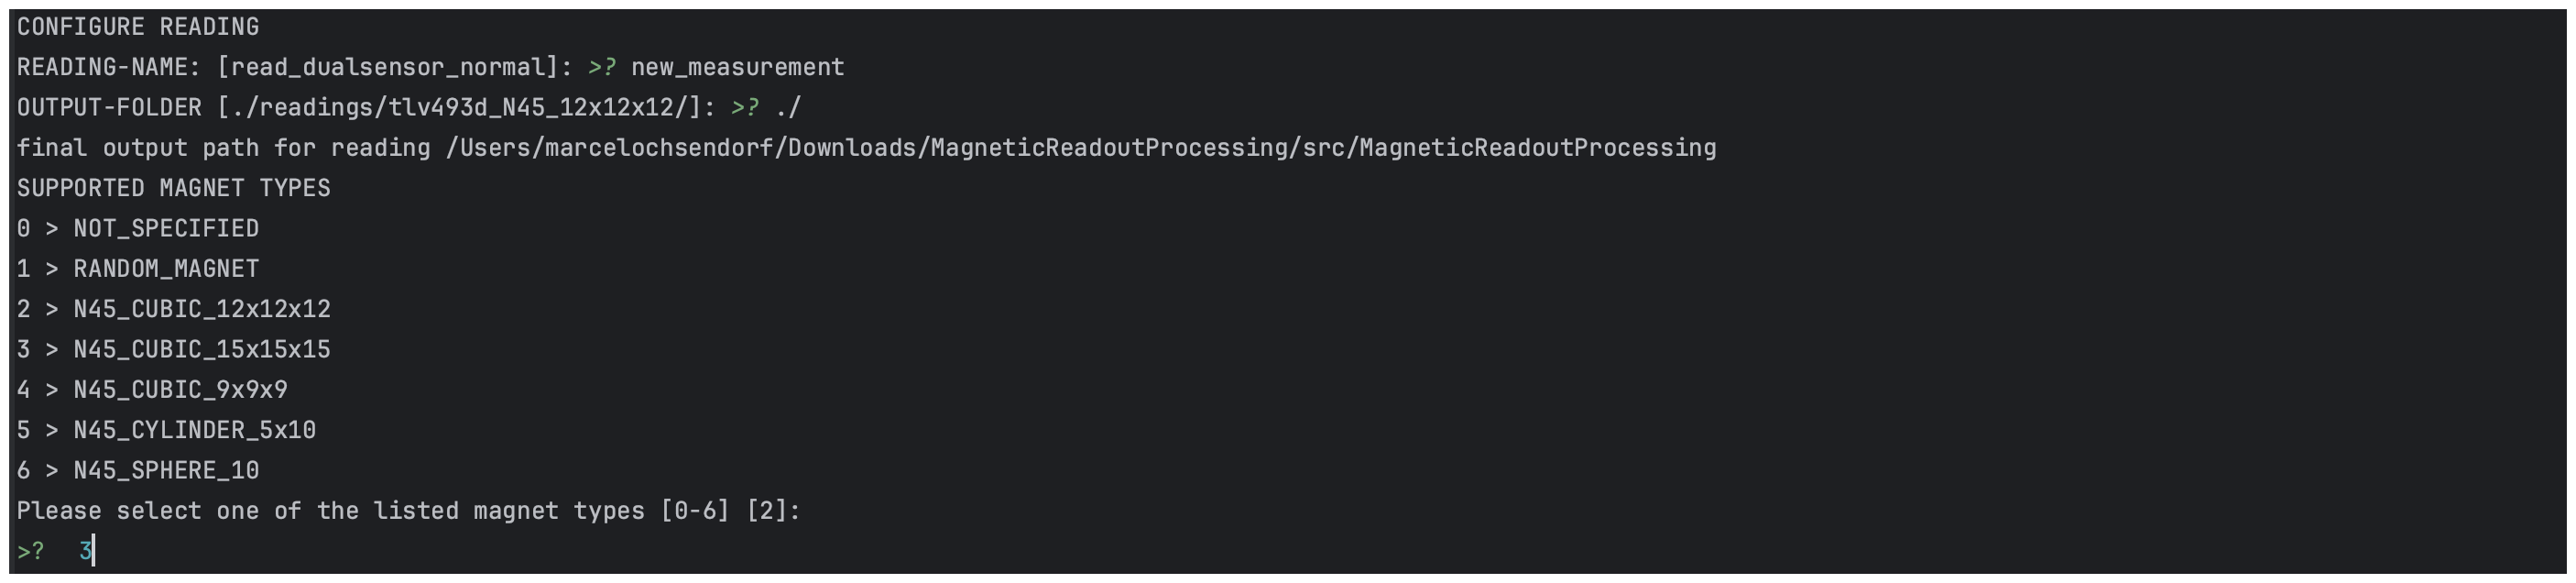
\includegraphics{./generated_images/border_MRP_(+cli)_output_to_configure_a_new_measurement.png}
\caption{MRP \gls{cli} output to configure a new measurement
\label{MRP_(+cli)_output_to_configure_a_new_measurement.png}}
\end{figure}

In the first version of the \gls{mrp}-library, the user had to write his
own Python scripts even for short measurement and visualisation tasks.
However, this was already time-consuming for reading out a sensor and
configuring the measurement parameters and metadata and quickly required
more than 100 lines of new Python code.

Although such examples are provided in the documentation, it must be
possible for programming beginners in particular to use them. To
simplify these tasks, a \gls{cli}
\ref{Example_measurement_analysis_pipeline.png} was implemented. The
libaray \gls{cli} implements the following functionalities:

\begin{itemize}
\tightlist
\item
  Detection of connected sensors
\item
  Configuration of measurement series
\item
  Recording of measured values from stored measurement series
\item
  Simple commands for checking recorded measurement series and their
  data
\end{itemize}

Thanks to this functionality of the \gls{cli}, it is now possible to
connect a sensor to the \gls{pc}, configure a measurement series with it
and run it at the end. The result is an exported file with the measured
values. These can then be read in again using the
\passthrough{\lstinline!MRPReading!} module and processed further. The
following bash code \ref{lst:mrpcli_config_run} shows the setup
procedure in detail:

\begin{lstlisting}[language=bash, caption={CLI example for configuring a measurement run}, label=lst:mrpcli_config_run]
# CLI EXAMPLE FOR CONFIGURING A MEASUREMENT RUN
## CONFIGURE THE SENSOR TO USE
$ MRPcli config setupsensor testcfg
> 0 - Unified Sensor 386731533439 - /dev/cu.usbmodem3867315334391
> Please select one of the found sensors [0]:
> sensor connected: True 1243455
## CONFIGURE THE MEASUREMENT
$ MRPcli config setup testcfg
> CONFIGURE testcfg
> READING-NAME: [testreading]: testreading
> OUTPUT-FOLDER [/cli/reading]: /tmp/reading_folder_path
> NUMBER DATAPOINTS: [1]: 10
> NUMBER AVERAGE READINGS PER DATAPOINT: [1]: 100
# RUN THE CONFIGURED MEASUREMENT
$ MRPcli measure run
> STARTING MEASUREMENT RUN WITH FOLLOWING CONFIGS: ['testcfg']
> config-test: OK
> sensor-connection-test: OK
> START MEASUREMENT CYCLE
> sampling 10 datapoints with 100 average readings
> SID:0 DP:0 B:47.359mT TEMP:23.56
> ....
> dump_to_file testreading_ID:525771256544952_SID:0_MAG:N45_CUBIC_12x12x12.mag.json
\end{lstlisting}

\hypertarget{programmable-data-processing-pipeline}{%
\section{Programmable Data Processing
Pipeline}\label{programmable-data-processing-pipeline}}

After it is easy for users to carry out measurements using the
\gls{cli}, the next logical step is to analyse the recorded data. This
can involve one or several hundred data records. Again, the procedure
for the user is to write their own evaluation scripts using the
\gls{mrp}-library.

This is particularly useful for complex analyses or custom algorithms,
but not necessarily for simple standard tasks such as bias compensation
or graphical plot outputs.

\begin{figure}
\centering
\includegraphics{./generated_images/border_Example_measurement_analysis_pipeline.png}
\caption{Example measurement analysis pipeline
\label{Example_measurement_analysis_pipeline.png}}
\end{figure}

For this purpose, a further \gls{cli} application was created, which
enables the user to create and execute complex evaluation pipelines for
measurement data without programming. The example
\ref{Example_measurement_analysis_pipeline.png} shows a typical
measurement data analysis pipeline, which consists of the following
steps:

\begin{enumerate}
\def\labelenumi{\arabic{enumi}.}
\tightlist
\item
  Import the measurements
\item
  Determine sensor bias value from imported measurements using a
  reference measurement
\item
  Apply linear temperature compensation
\item
  Export the modified measurements
\item
  Create a graphical plot of all measurements with standard deviation
\end{enumerate}

In order to implement such a pipeline, the
\passthrough{\lstinline!yaml!} file format was chosen for the definition
of the pipeline, as this is for non programmers to understand and can
also be easily edited with a plain text editor. Detailed examples can be
found in the documentation
\cite{MagneticReadoutProcessingReadTheDocs}. The pipeline definition
consists of sections which execute the appropriate Python commands in
the background.

The signatures in the \passthrough{\lstinline!yaml!} file are called
using \passthrough{\lstinline!reflection!} and a real-time search of the
loaded \passthrough{\lstinline!global()!} functions symbol table
\cite{PythonGlobalSymbolTable}. This system makes almost all Python
functions available to the user. To simplify use, a pre-defined list of
verified functions for use in pipelines is listed in the documentation
\cite{MagneticReadoutProcessingReadTheDocs}. The following pipeline
definition \ref{lst:mrpuddp_example_yaml} shows the previously defined
steps \ref{Example_measurement_analysis_pipeline.png} as
\passthrough{\lstinline!yaml!} syntax.

\begin{lstlisting}[caption={Example YAML code of an user defined processing pipeline with six stages linked together}, label=lst:mrpuddp_example_yaml]
stage import_readings:
  function: import_readings
  parameters:
    IP_input_folder: ./readings/fullsphere/
    IP_file_regex: 360_(.)*.mag.json

stage import_bias_reading:
  function: import_readings
  parameters:
    IP_input_folder: ./readings/fullsphere/
    IP_file_regex: bias_reading.mag.json

stage apply_bias_offset:
  function: apply_sensor_bias_offset
  parameters:
    bias_readings: stage import_bias_reading # USE RESULT FROM FUNCTION import_bias_reading
    readings_to_calibrate: stage import_readings

stage apply_temp_compensation:
  function: apply_temperature_compensation
  parameters:
    readings_to_calibrate: stage import_readings # USE RESULT FROM FUNCTION import_readings

stage plot_normal_bias_offset:
  function: plot_readings
  parameters:
    readings_to_plot: stage apply_temp_compensation
    IP_export_folder: ./readings/fullsphere/plots/
    IP_plot_headline_prefix:  Sample N45 12x12x12 magnets calibrated

stage export_readings:
  function: export_readings
  parameters:
    readings_to_plot: stage apply_temp_compensation
    IP_export_folder: ./readings/fullsphere/plots/
\end{lstlisting}

Each pipeline step is divided into \passthrough{\lstinline!stages!},
which contain a name, the function to be executed and its parameters.

\newpage

The various steps are then linked by using the
\passthrough{\lstinline!stage <name>!} makro as input parameter of the
next function to be executed (see comments in
\ref{lst:mrpuddp_example_yaml}).

It is therefore also possible to use the results of one function in
several others without them directly following each other. The
disadvantages of this system are the following:

\begin{itemize}
\tightlist
\item
  No circular parameter dependencies
\item
  Complex determination of the execution sequence of the steps
\end{itemize}

To determine the order of the pipeline steps, the parser script created
converts them into one problem of the graph theories. Each step
represents a node in the graph and the steps referred to by the input
parameter form the edges. After several simplification steps,
determination of possible start steps and repeated traversal, the final
execution sequence can be determined in the form of a call tree
\ref{Example_result_of_an_step_execution_tree_from_user_defined_processing_pipeline.png}.
The individual steps are then executed along the graph. The intermediate
results and the final results
\ref{Pipeline_output_files_after_running_example_pipeline_on_a_set_of_readings.png}
are saved for optional later use.

\begin{figure}
\centering
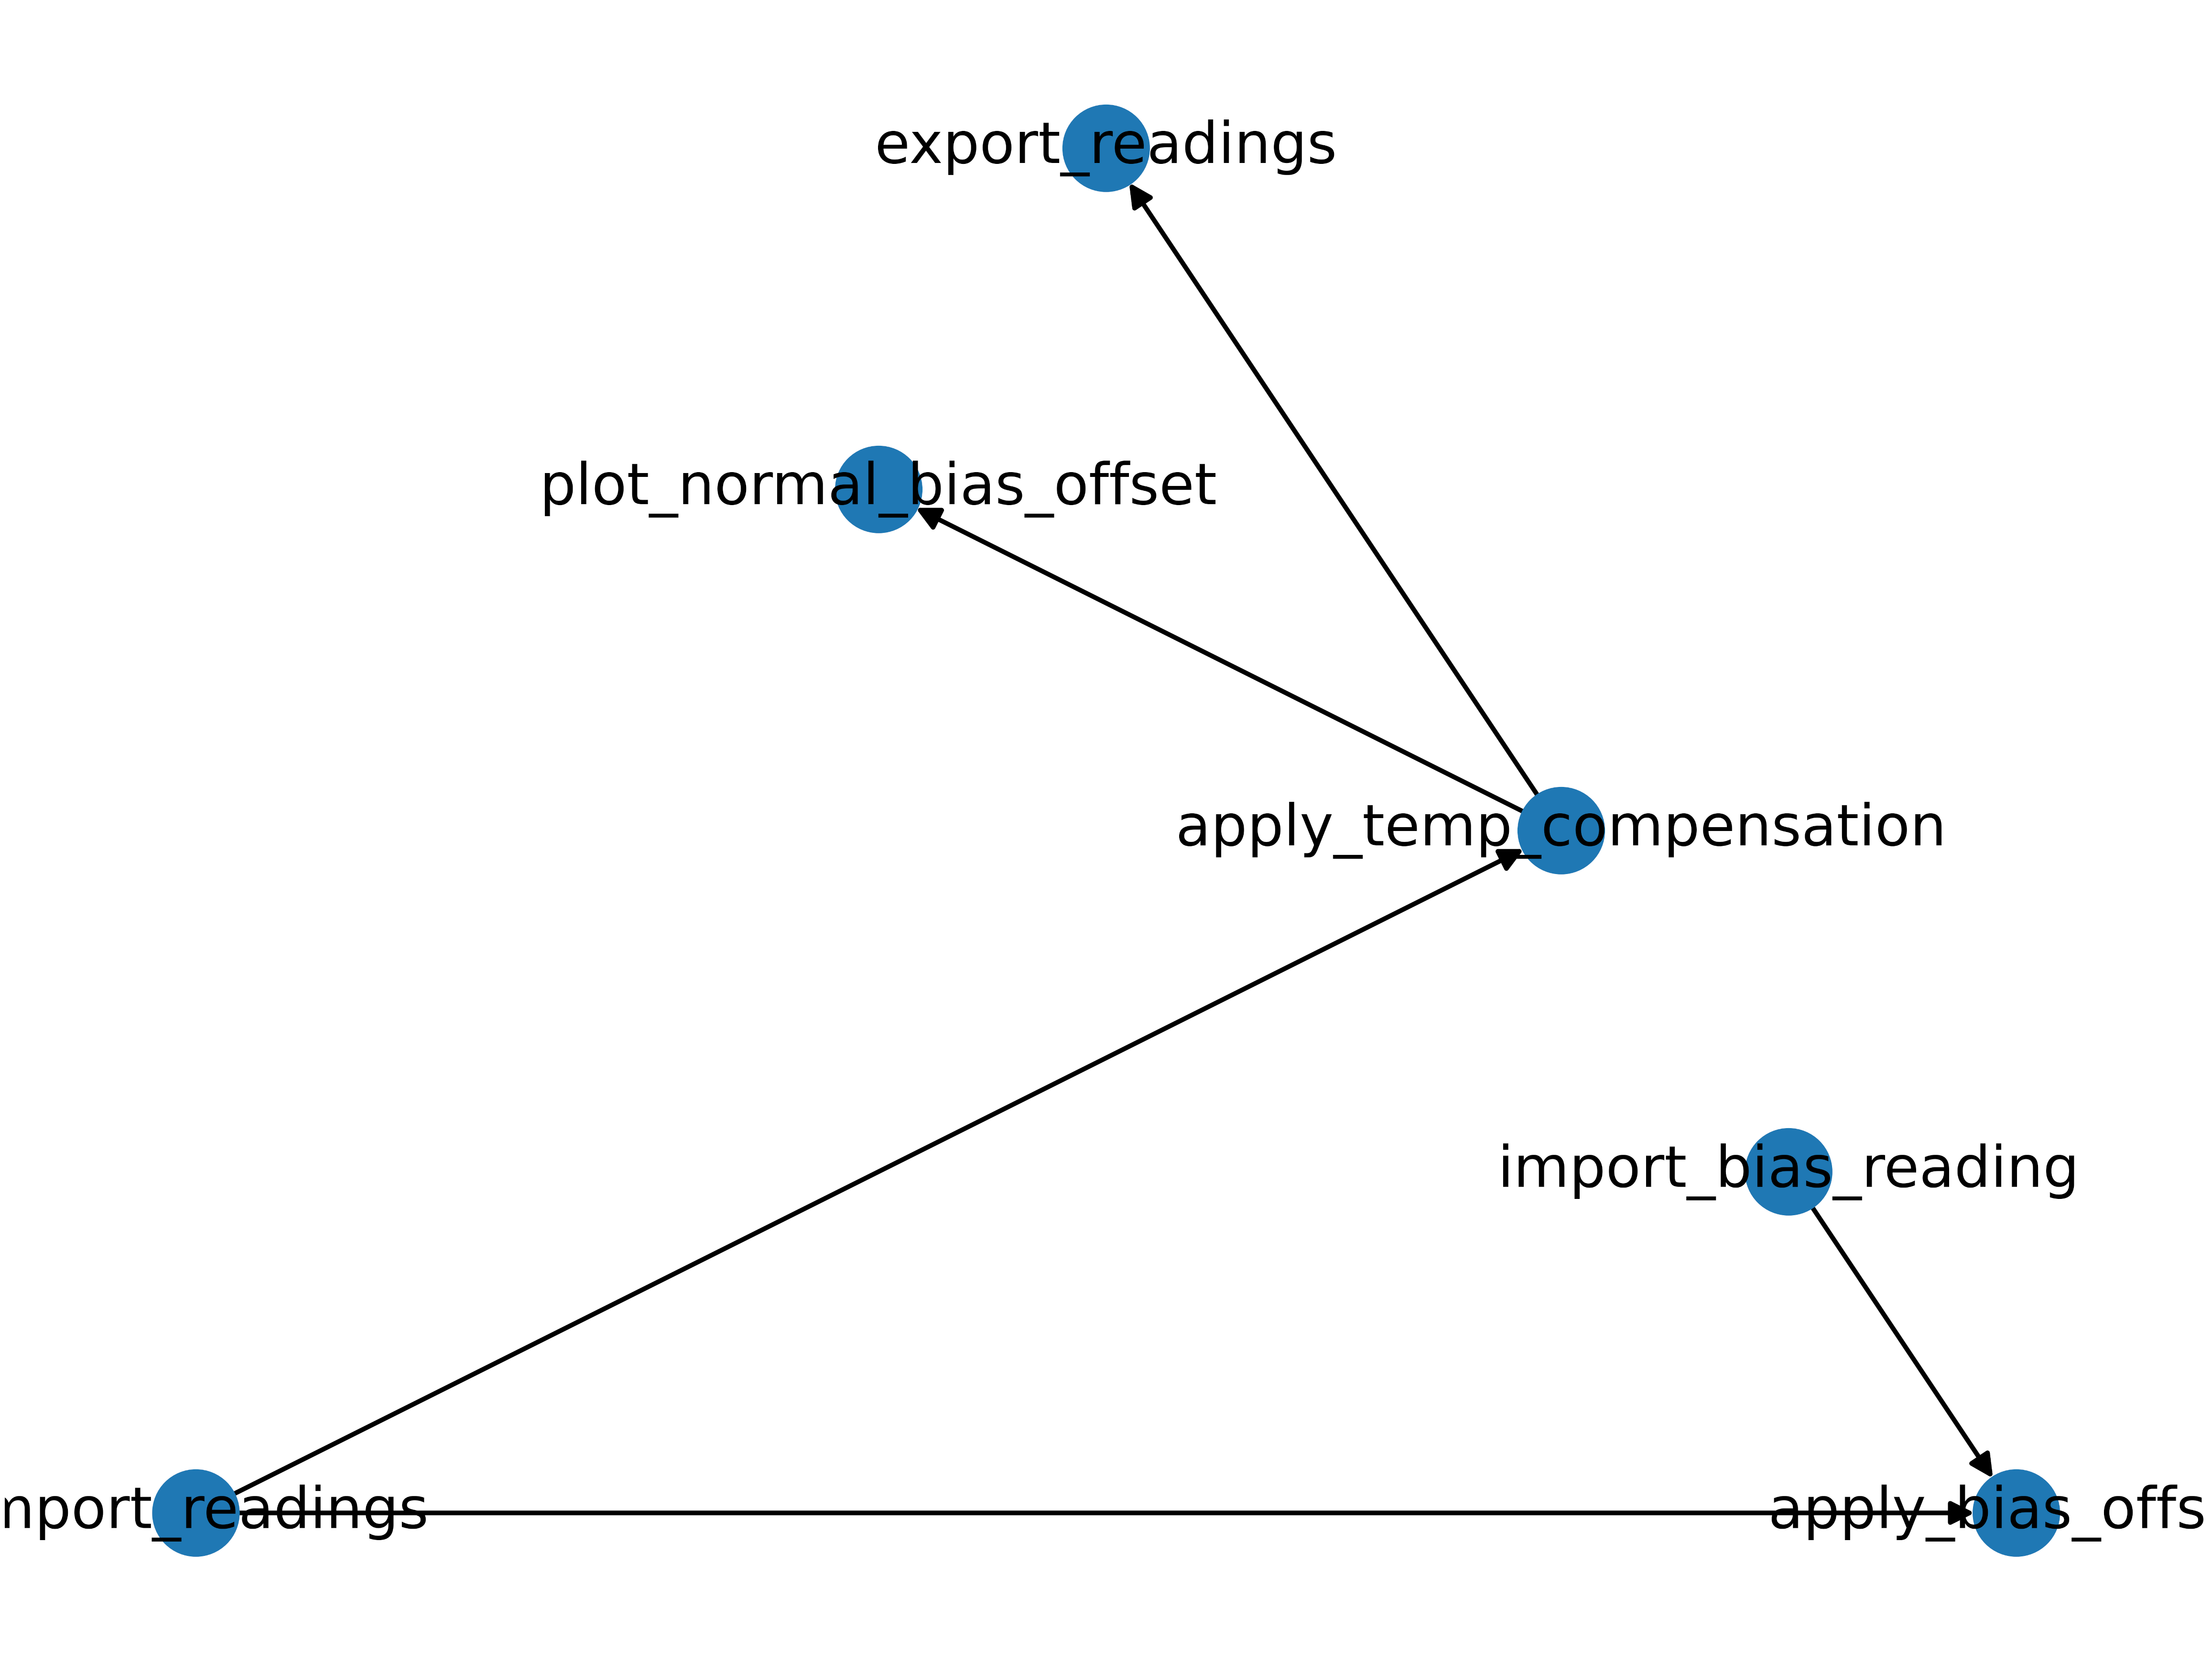
\includegraphics{./generated_images/border_Example_result_of_an_step_execution_tree_from_user_defined_processing_pipeline.png}
\caption{Example result of an step execution tree from user defined
processing pipeline
\label{Example_result_of_an_step_execution_tree_from_user_defined_processing_pipeline.png}}
\end{figure}

\begin{figure}
\centering
\includegraphics{./generated_images/border_Pipeline_output_files_after_running_example_pipeline_on_a_set_of_readings.png}
\caption{Pipeline output files after running example pipeline on a set
of readings
\label{Pipeline_output_files_after_running_example_pipeline_on_a_set_of_readings.png}}
\end{figure}

\hypertarget{testing}{%
\section{Testing}\label{testing}}

\begin{figure}
\centering
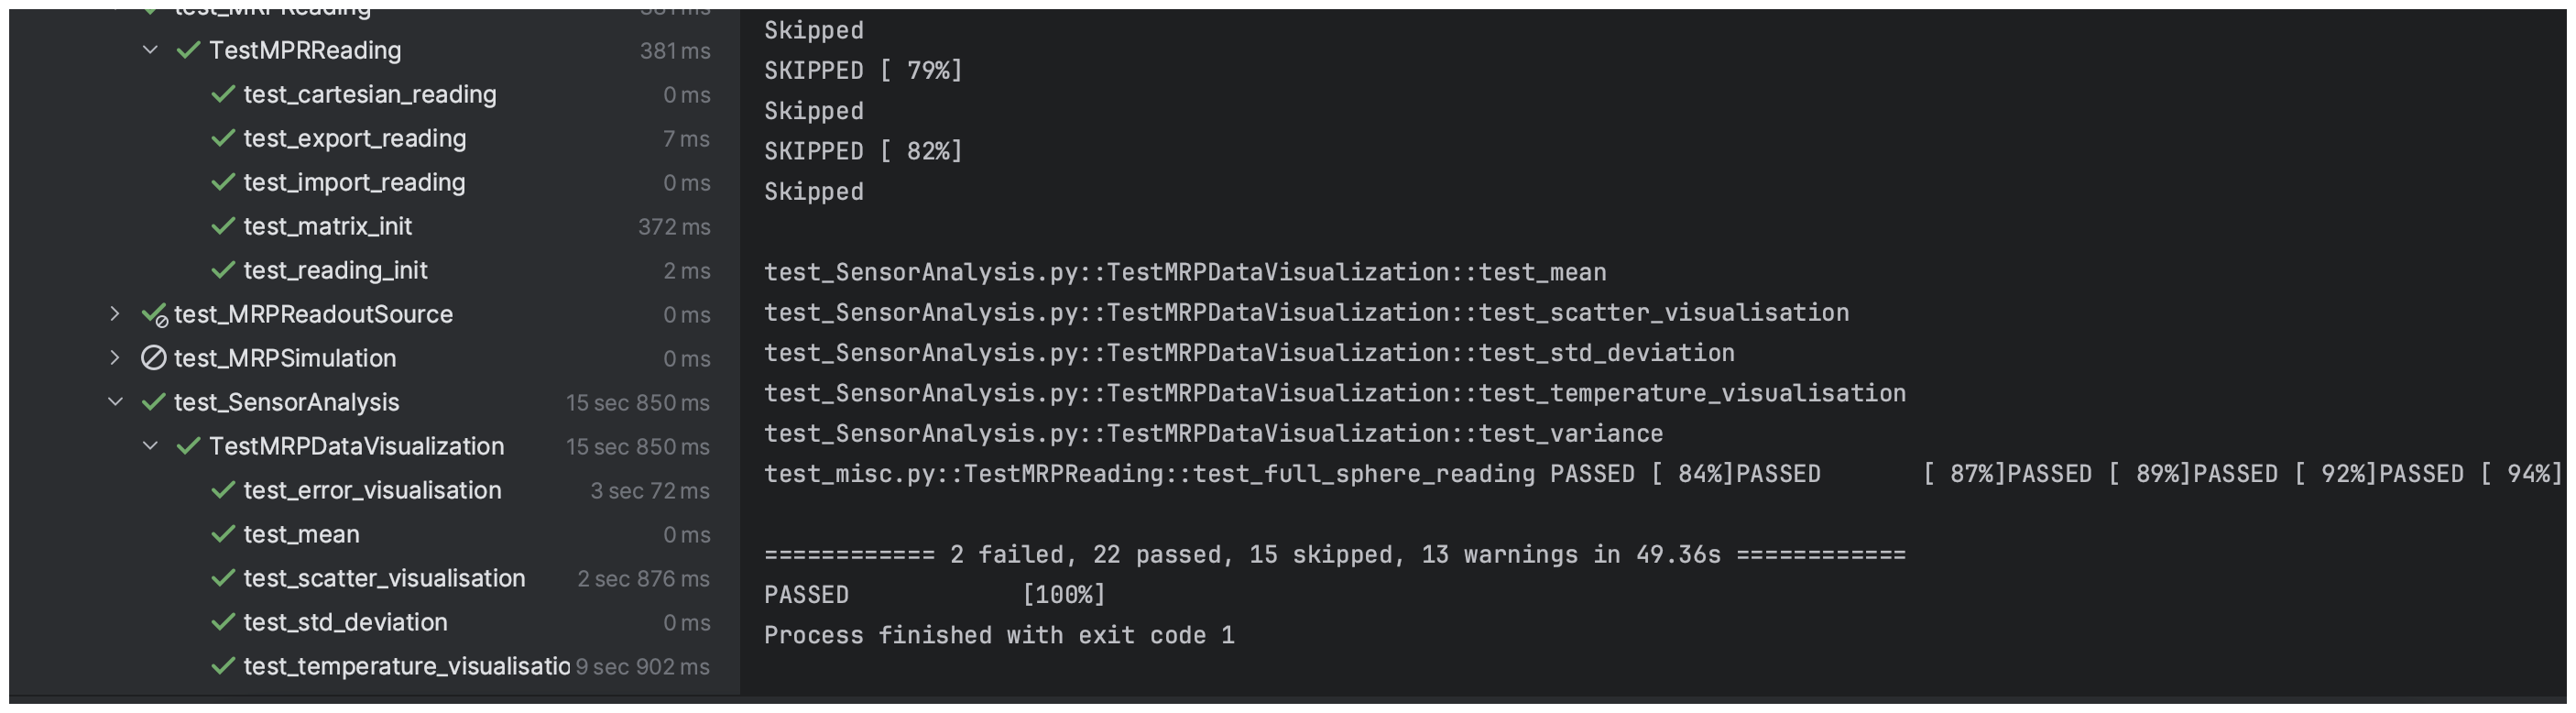
\includegraphics{./generated_images/border_MRP_library_test_results_for_different_submodules_executed_in_PyCharm_(+ide).png}
\caption{MRP library test results for different submodules executed in
PyCharm \gls{ide}
\label{MRP_library_test_results_for_different_submodules_executed_in_PyCharm_(+ide).png}}
\end{figure}

Software tests in libraries offer numerous advantages for improving
quality and efficiency. Software tests make it possible to identify
errors and vulnerabilities before the software is released as a new
version.

This significantly improves the reliability of \gls{mrp}-library
applications. Tests also ensures consistent and reliable performance,
which is particularly important when libraries are used by different
users and for different usecases.

During the development of the \gls{mrp}-library, test cases were also
created for all important functionalities and usecases. The test
framework \passthrough{\lstinline!PyTest!} \cite{PyTest} was used
for this purpose, as it offers direct integration in most \gls{ide}s
(see
\ref{MRP_library_test_results_for_different_submodules_executed_in_PyCharm_(+ide).png})
and also because it provides detailed and easy-to-understand test
reports as output in order to quickly identify and correct errors. It
also allows to tag tests, which is useful for grouping tests or
excluding certain tests in certain build environment scenarios. Since
all intended usecases were mapped using the test cases created, the code
of the test cases could later be used in slightly simplified variants
\ref{lst:pytest_example_code} as examples for the documentation.

\begin{lstlisting}[language=Python, caption={Example pytest class for testing MRPReading module functions}, label=lst:pytest_example_code]
class TestMPRReading(unittest.TestCase):
  # PREPARE A INITIAL CONFIGURATION FILE FOR ALL FOLLOWING TEST CASES IN THIS FILE
  def setUp(self) -> None:
    self.test_folder: str = os.path.join(os.path.dirname(os.path.abspath(__file__)), "tmp")
    self.test_file:str = os.path.join(self.import_export_test_folderpath, "tmp")

  def test_matrix(self):
    reading: MRPReading = MRPSimulation.generate_reading()
    matrix: np.ndarray = reading.to_numpy_matrix()
    n_phi: float = reading.measurement_config.n_phi
    n_theta: float = reading.measurement_config.n_theta
    # CHECK MATRIX SHAPE
    self.assertTrue(matrix.shape != (n_theta,))
    self.assertTrue(len(matrix.shape) <= n_phi)

  def test_export_reading(self) -> None:
    reading: MRPReading = MRPSimulation.generate_reading()
    self.assertIsNotNone(reading)
    # EXPORT READING TO A FILE
    reading.dump_to_file(self.test_file)

  def test_import_reading(self):
    # CREATE EMPTY READING AND LOAD FROM FILE
    reading_imported:MRPReading = MRPReading.MRPReading(None)
    reading_imported.load_from_file(self.test_file)
    # COMPARE
    self.assertIsNotNone(reading_imported.compare(MRPSimulation.generate_reading()))
\end{lstlisting}

One problem, is the parts of the \gls{mrp}-library that require direct
access to external hardware. These are, for example, the
\passthrough{\lstinline!MRPHal!} and
\passthrough{\lstinline!MRPHalRest!} modules, which are required to read
out sensors connected via the network. Two different approaches were
used here. In the case of local development, the test runs were carried
out on a \gls{pc} that can reach the network hardware and thus the test
run could be carried out with real data.

\newpage

In the other scenario, the tests are to be carried out before a new
release in the repository on the basis of
\passthrough{\lstinline!Github Actions!} \cite{GithubActions}. Here
there is the possibility to host local runner software, which then has
access to the hardware, but then a \gls{pc} must be permanently
available for this task. Instead, the hardware sensors were simulated by
software and executed via virtualisation on the systems provided by
\passthrough{\lstinline!Github Actions!}.

\hypertarget{package-distribution}{%
\section{Package Distribution}\label{package-distribution}}

\begin{figure}
\centering
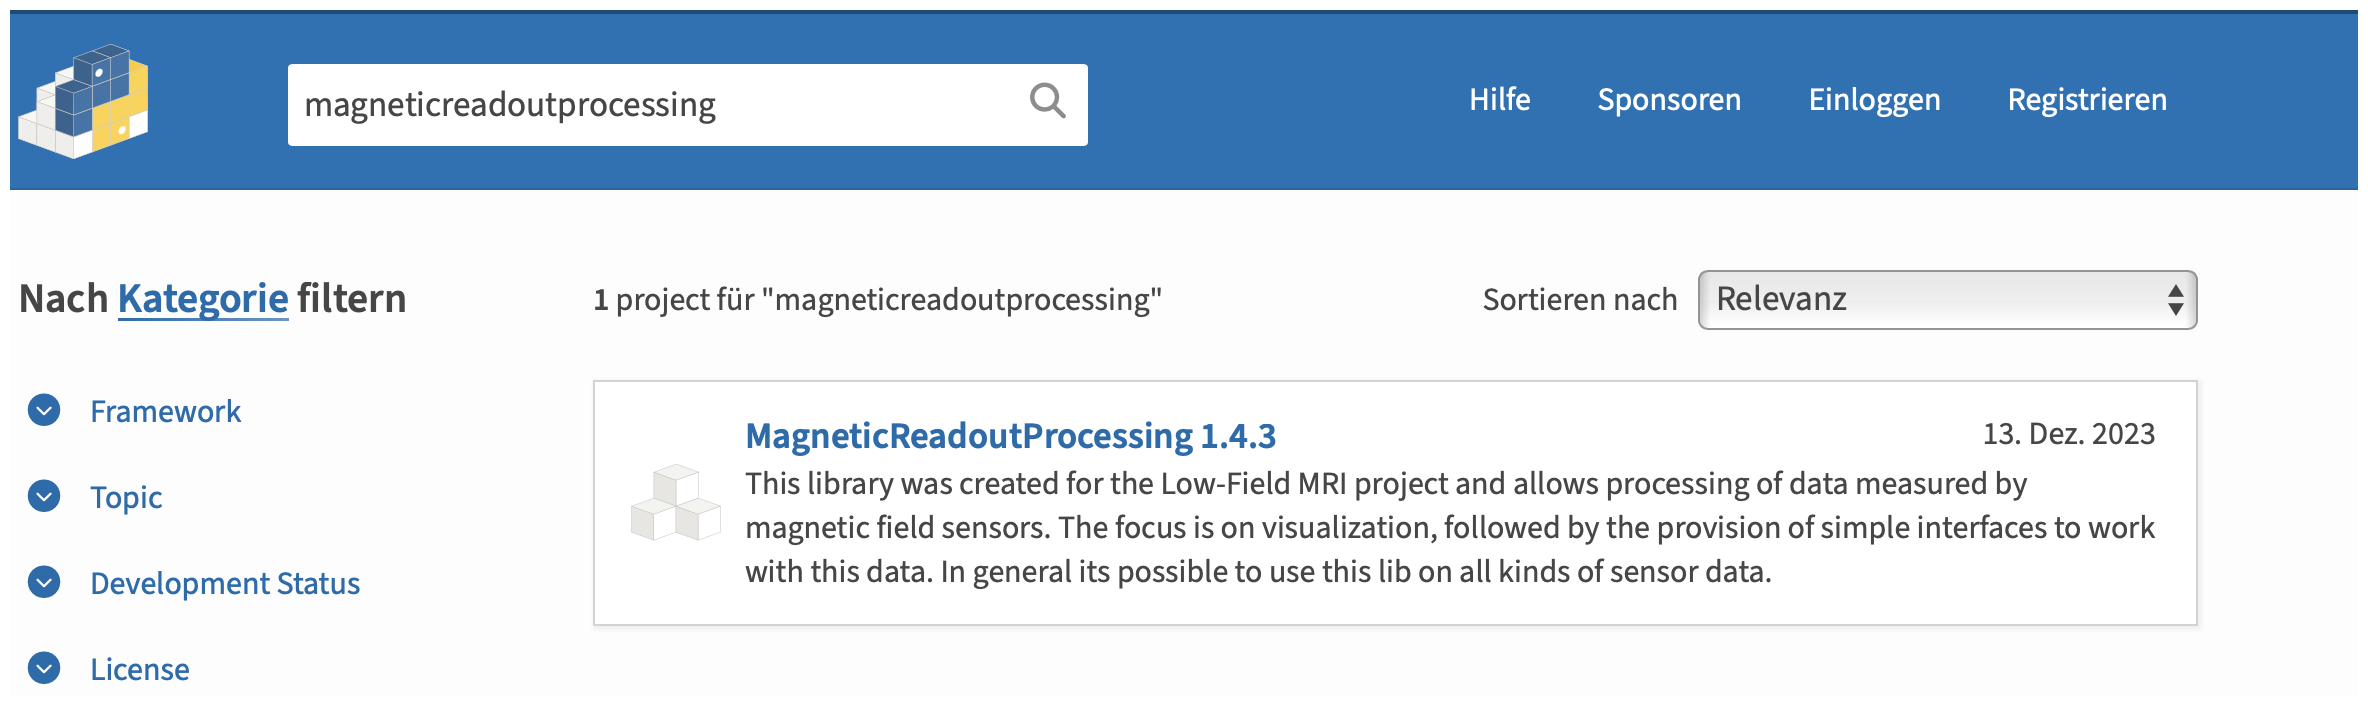
\includegraphics{./generated_images/border_MagneticReadoutProcessing_library_hosted_on_PyPi.png}
\caption{MagneticReadoutProcessing library hosted on PyPi
\label{MagneticReadoutProcessing_library_hosted_on_PyPi.png}}
\end{figure}

One important point that improves usability for users is the simple
installation of all \gls{mrp} modules. As it was created in the Python
programming language, there are several public package registry where
users can provide their software modules. Here,
\passthrough{\lstinline!PyPi!}\cite{PyPI}
\ref{MagneticReadoutProcessing_library_hosted_on_PyPi.png}
\cite{MagneticReadoutProcessingPyPI} is the most commonly used
package registry and offers direct support for the package installation
programm \gls{pip} \ref{lst:setup_lib_with_pip}.

\gls{pip} not only manages possible package dependencies, but also
manages the installation of different versions of a package. In
addition, the version compatibility is also checked during the
installation of a new package, which can be resolved manually by the
user in the event of conflicts.

\begin{lstlisting}[language=bash, caption={Bash commands to install the MagneticReadoutProcessing library using pip}, label=lst:setup_lib_with_pip]
# https://pypi.org/project/MagneticReadoutProcessing/
# install the latest version
$ pip3 install MagneticReadoutProcessing
# install the specific version 1.4.0
$ pip3 install MagneticReadoutProcessing==1.4.0
\end{lstlisting}

To make the \gls{mrp} file structure compatible with the package
registry, Python provides separate installation routines that build a
package in an isolated environment and then provide an installation
\passthrough{\lstinline!wheel!} archive. This can then be uploaded to
the package registry. Since the \gls{mrp}-library requires additional
Python dependencies (e.g.~\passthrough{\lstinline!numpy!},
\passthrough{\lstinline!matplotlib!} packages), which cannot be assumed
to be already installed on the target system, these must be installed
prior to the actual installation. These can be specified in the library
installation configuration \passthrough{\lstinline!setup.py!}
\ref{lst:setup_py_req} for this purpose.

\begin{lstlisting}[language=Python, caption={setup.py with dynamic requirement parsing used given requirements.txt}, label=lst:setup_py_req]
# dynamic requirement loading using 'requirements.txt'
req_path = './requirements.txt'
with pathlib.Path(req_path).open() as requirements_txt:
  install_requires = [str(requirement) for requirement in pkg_resources.parse_requirements(requirements_txt)]

setup(name='MagneticReadoutProcessing',
  version='1.4.3',
  url='https://github.com/LFB-MRI/MagnetCharacterization/',
  packages= ['MRP', 'MRPcli', 'MRPudpp', 'MRPproxy'],
  install_requires=install_requires,
  entry_points={
    'console_scripts': [
      'MRPCli = MRPcli.cli:run',
      'MRPUdpp = MRPudpp.uddp:run',
      'MRPproxy = MRPproxy.mrpproxy:run'
    ]
  }
)
\end{lstlisting}

To make the \gls{cli} scripts written in Python easier for the user to
execute without having to use the \passthrough{\lstinline!python3!}
prefix. This has been configured in the installation configuration using
the \passthrough{\lstinline!entry\_points!} option, and the following
commands are available to the user:

\begin{itemize}
\tightlist
\item
  \passthrough{\lstinline!MRPcli --help!} instead of
  \passthrough{\lstinline!python3 cli.py --help!}
\item
  \passthrough{\lstinline!MRPudpp --help!} instead of
  \passthrough{\lstinline!python3 udpp.py --help!}
\item
  \passthrough{\lstinline!MRPproxy --help!} instead of
  \passthrough{\lstinline!python3 proxy.py --help!}
\end{itemize}

In addition, these commands are available globally in the system without
the terminal shell being located in the \gls{mrp}-library folder.

\hypertarget{documentation}{%
\subsection{Documentation}\label{documentation}}

In order to provide comprehensive documentation for the enduser, the
source code was documented using
Python-\passthrough{\lstinline!docstrings!}
\cite{PythonDocstringReference} and the Python 3.5 type annotations:

\begin{itemize}
\tightlist
\item
  Function description
\item
  Input parameters, using \passthrough{\lstinline!param!} and
  \passthrough{\lstinline!type!}
\item
  Return value, using \passthrough{\lstinline!returns!},
  \passthrough{\lstinline!rtype!}
\end{itemize}

The use of type annotations also simplifies further development, as
modern \gls{ide}s can more reliably display possible methods to the user
as an assistance. \ref{lst:pydocstring}

\begin{lstlisting}[language=Python, caption={Documentation using Python docstring example}, label=lst:pydocstring]
# MRPDataVisualisation.py - example docstring
def plot_temperature(_readings: [MRPReading.MRPReading], _title: str = '', _filename: str = None, _unit: str = "degree C") -> str:
  """
  Plots a temperature bar graph of the reading data entries as figure
  :param _readings: readings to plot
  :type _readings: list(MRPReading.MRPReading)
  :param _title: Title text of the figure, embedded into the head
  :type _title: str
  :param _filename: export graphic to an given absolute filepath with .png
  :type _filename: str
  :returns: returns the abs filepath of the generated file
  :rtype: str
  """
  if _readings is None or len(_readings) <= 0:
      raise MRPDataVisualizationException("no readings in _reading given")
  num_readings = len(_readings)
  # ...
\end{lstlisting}

Since \passthrough{\lstinline!docstrings!} only document the source
code, but do not provide simple how-to-use instructions, the
documentation framework \passthrough{\lstinline!Sphinx!}
\cite{SphinxDocumentation} was used for this purpose. This framework
makes it possible to generate \gls{html} or \gls{pdf} documentation from
various source code documentation formats, such as the used
\passthrough{\lstinline!docstrings!}.

These are converted into a Markdown format in an intermediate step and
this also allows to add further user documentation such as examples or
installation instructions. In order to make the documentation created by
\passthrough{\lstinline!Sphinx!} accessible to the user, there are, as
with the package management by \passthrough{\lstinline!PyPi!} services,
which provide the \gls{mrp}-library documentation online.

Once the finished documentation has been generated from static
\gls{html} files, it is stored in the project repository. Another
publication option is to host the documentation via online services such
as \passthrough{\lstinline!ReadTheDocs!} \cite{ReadTheDocs}, where
users can make documentation for typical software projects available to
others.

The documentation has also been uploaded to
\passthrough{\lstinline!ReadTheDocs!}
\cite{MagneticReadoutProcessingReadTheDocs} and linked in the
repository and on the overview page
\ref{MagneticReadoutProcessing_documentation_hosted_on_ReadTheDocs.png}
on \passthrough{\lstinline!PyPi!}.

The process of creating and publishing the documentation has been
automated using \passthrough{\lstinline!GitHub Actions!}, so that it is
always automatically kept up to date with new features.

\begin{figure}
\centering
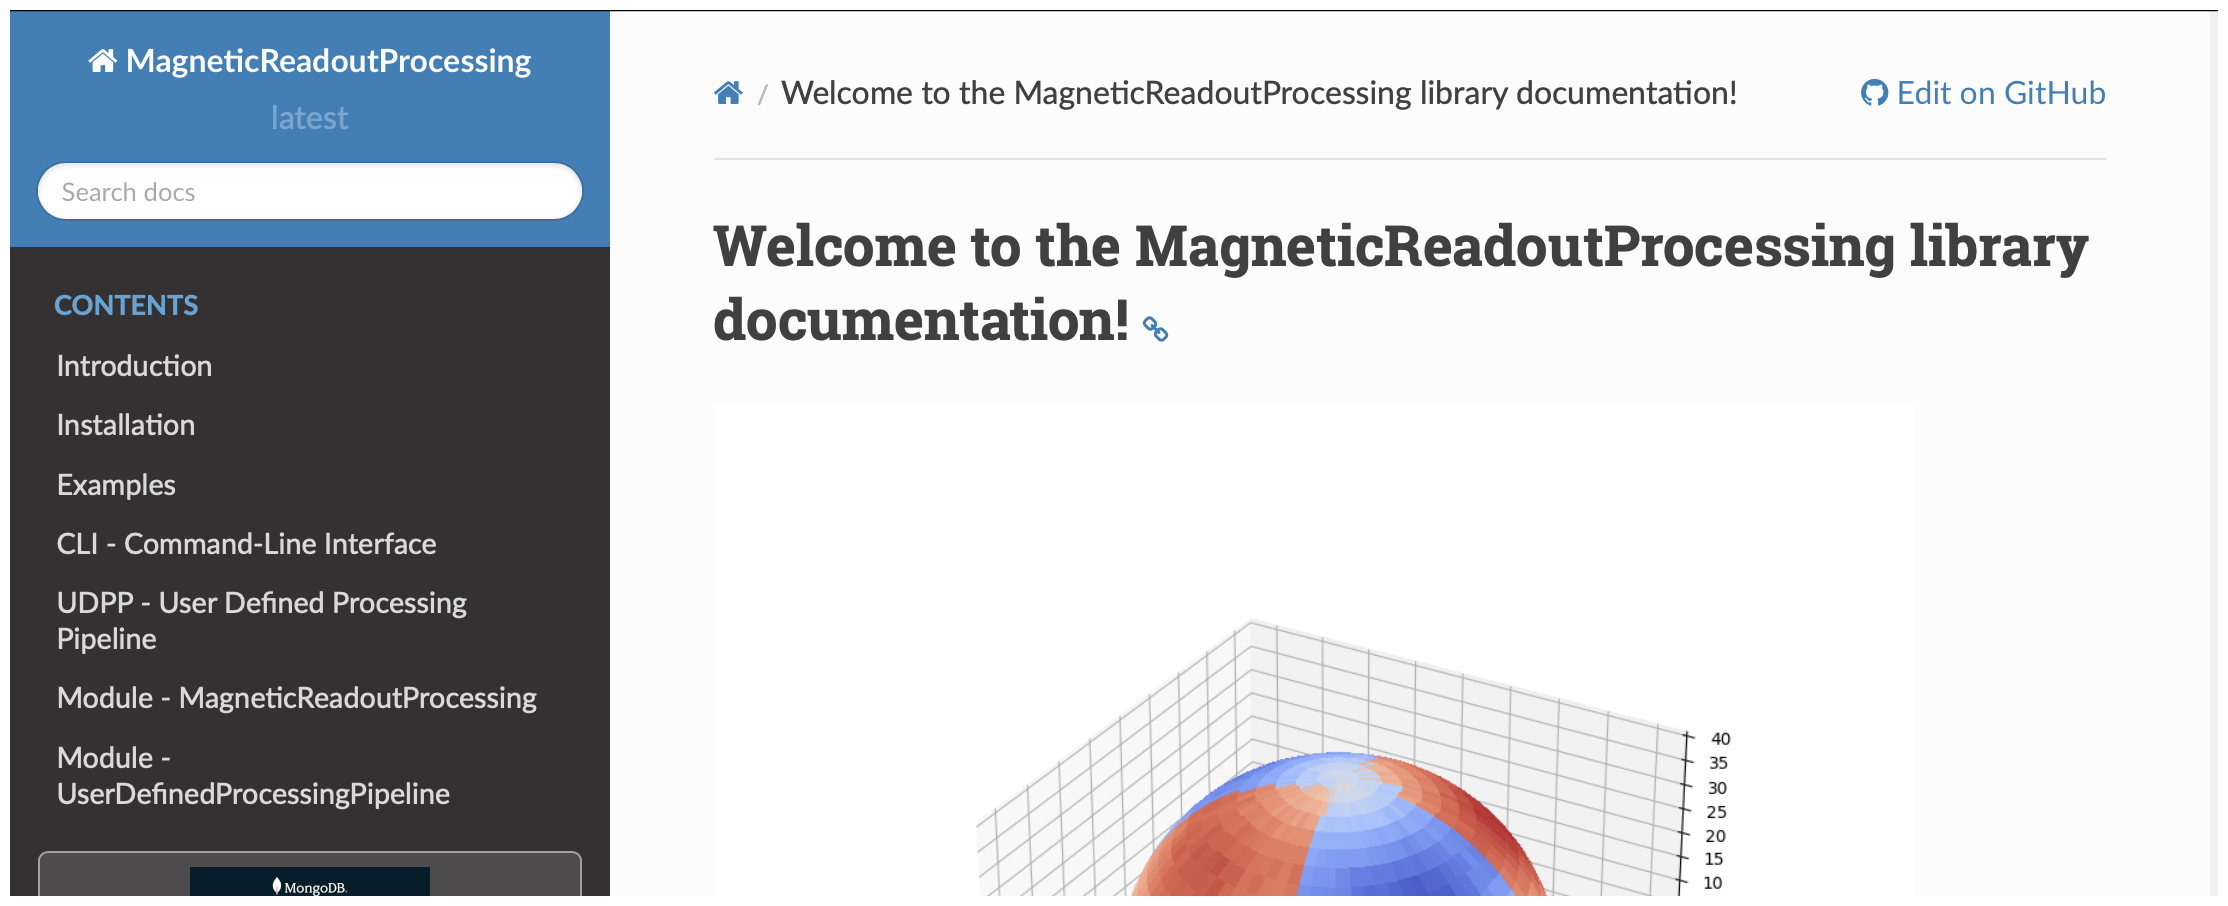
\includegraphics{./generated_images/border_MagneticReadoutProcessing_documentation_hosted_on_ReadTheDocs.png}
\caption{MagneticReadoutProcessing documentation hosted on ReadTheDocs
\label{MagneticReadoutProcessing_documentation_hosted_on_ReadTheDocs.png}}
\end{figure}

\hypertarget{evaluation}{%
\chapter{Evaluation}\label{evaluation}}

This work successfully implemented a universal hardware and software
framework for the automated characterisation of permanent magnets. This
framework consists of a low-cost hardware interface that supports
various magnetic field sensors and a library for automating and
analysing the measurement data. The process of this framework comprises
several steps, which will be explain below:

\begin{enumerate}
\def\labelenumi{\arabic{enumi}.}
\item
  \textbf{Hardware preperation}: Users can prepare measurements using
  the implemented framework. This includes the placement of the sensors
  and the selection of the relevant parameters for the characterisation
  of the permanent magnets.
\item
  \textbf{Configuration of the measurement}: The software provides a
  user-friendly interface for configuring the measurement parameters.
  Users can make the desired settings here and customise the framework
  to their specific requirements.
\item
  \textbf{Custom algorithm implementation}: An important contribution of
  the \gls{mrp} ecosystem is the possibility for users to implement
  their own algorithm for data analysis. This allows customisation to
  specific research questions or experimental requirements.
\item
  \textbf{Execution of analysis pipeline}: The analysis pipeline can
  then be executed with the implemented algorithm. The collected
  measurement data is automatically processed and analysed to extract
  characteristic parameters of the permanent magnets.
\end{enumerate}

This process covers all the essential functionalities required for a
comprehensive characterisation of permanent magnets. These were
previously described in the Usecases \ref{usecases} chapter. The
developed framework not only offers a cost-effective and flexible
hardware solution, but also enables customisation of the analysis
algorithms to meet the requirements of different research projects.

\hypertarget{hardware-preperation}{%
\section{Hardware preperation}\label{hardware-preperation}}

\begin{figure}
\centering
\includegraphics{./generated_images/border_Ten_numbered_test_magnets_in_separate_holders.png}
\caption{Ten numbered test magnets in separate holders
\label{Ten_numbered_test_magnets_in_separate_holders.png}}
\end{figure}

For the hardware setup, the 3D-Fullsphere\ref{d-fullsphere} sensor was
used for the evaulation of the framework. As this is equipped with an
exchangeable magnetic holder mount, suitable holders are required for
the magnets to be measured. Ten random
\passthrough{\lstinline!N45 12x12x12mm!} neodymium magnets were used,
which are shown in figure
\ref{Ten_numbered_test_magnets_in_separate_holders.png}.

These were placed in modified 3D printed holders
\ref{Ten_numbered_test_magnets_in_separate_holders.png} and then
numbered. This allows them to be matched to the measurement results
later.

\hypertarget{configuration-of-the-measurement}{%
\section{Configuration of the
Measurement}\label{configuration-of-the-measurement}}

The configured hardware was then connected to the host system using the
\passthrough{\lstinline!MRPcli config setupsensor!}-\gls{cli} command.
Afterwards, the measurement was configured for an measurement run, using
the following configuration commands
\ref{lst:evaluation_measurement_config}.

\newpage

\begin{lstlisting}[language=bash, caption={Measurement configuration for evaluation measurement}, label=lst:evaluation_measurement_config]
## CONFIGURE THE MEASUREMENT
$ MRPcli config setup eval_measurement_config
> READING-NAME: 360_eval_magnet_<id>
> OUTPUT-FOLDER: ./readings/evaluation/ 
> NUMBER DATAPOINTS: 18 # FOR A FULLSPHERE READING USE MULTIBLE OF 18
> NUMBER AVERAGE READINGS PER DATAPOINT: 10
\end{lstlisting}

The \passthrough{\lstinline!MRPcli measure run!} command was then called
up for each individual magnet to execute a measurement. After each run,
the \passthrough{\lstinline!READING-NAME!} parameter was filled with the
id of the next magnet so that all measurements could be assigned to the
physical magnets.

\hypertarget{custom-algorithm-implementation}{%
\section{Custom Algorithm
Implementation}\label{custom-algorithm-implementation}}

The next step for the user is the implementation of the filter algorithm
\ref{lst:custom_find_similar_values_algorithm}. This can have any
function signature and is implemented in the file
\passthrough{\lstinline!UDPPFunctionCollection.py!}. This Python file is
loaded when the pipeline is started and all functions that are imported
here as a module or implemented directly can be called via the pipeline.
As this is a short algorithm, it was inserted directly into the file.

The parameter \passthrough{\lstinline!\_readings!} should later receive
the imported measurements from the
\passthrough{\lstinline!stage rawimport!}
\ref{lst:pipeline_mrp_evaluation_yaml} and the optional
\passthrough{\lstinline!IP\_return\_count!} parameter specifies the
number of best measurements that are returned. The return parameter is a
list of measurements containing the most similar measurements, measured
by the smallest distance between all measurements. The distance for each
measurement is determined using the center of gravity function
\passthrough{\lstinline!CoG!}, the length is then calculated from the
result vector. This value can then be used for sorting.

\begin{lstlisting}[language=Python, caption={User implemented custom find most similar readings algorithm}, label=lst:custom_find_similar_values_algorithm]
@staticmethod
def FindSimilarValuesAlgorithm(_readings: [MRPReading.MRPReading], IP_return_count: int = -1) -> [MRPReading.MRPReading]:
  import heapq
  import math
  heap = []
  # SET RESULT VALUE COUNT
  IP_return_count = max([int(IP_return_count),len(_readings)])
  if IP_return_count < 0:
      IP_return_count = len(_readings) / 5
  # CALCULATE TARGET VALUE: CENTER OF GRAVITY MAGNITUDE FOR ALL READINGS
  target_value = 0.0
  for idx, r in enumerate(_readings):
      cog_vecotr = MRPAnalysis.MRPAnalysis.calculate_center_of_gravity(r)
      # COMPUTE LENGTH OF VECTOR
      cog:float = math.sqrt(cog[0]**2 + cog[1]**2 cog[2]**2)
      target_value = target_value + cog
  target_value = target_value / len(_readings)
  # PUSH READINGS TO HEAP
  for value in _readings:
      # USE DIFF AS PRIORITY VALUE IN MIN-HEAP
      diff = abs(value - target_value)
      heapq.heappush(heap, (diff, value))
  # RETURN X BEST ITEMS FROM HEAP
  similar_values = [item[1] for item in heapq.nsmallest(IP_return_count, heap)]
  # CLEAN UP USED LIBRARIES AND RETURN RESULT
  del heapq
  del math
  return similar_values
\end{lstlisting}

The Python \passthrough{\lstinline!heapq!} \cite{heapq} module,
which implements a priority queue, is used for this purpose. The
calculated distances from the \passthrough{\lstinline!CoG!} value of the
measurements to are inserted into this queue. Subsequently, as many
elements of the queue are returned as defined by the
\passthrough{\lstinline!IP\_return\_count!} parameter. The actual
sorting was carried out by the queue in the background.

\hypertarget{execution-of-analysis-pipeline}{%
\section{Execution of Analysis
Pipeline}\label{execution-of-analysis-pipeline}}

Once the filter function has been implemented, it still needs to be
integrated into the analysis
pipeline\ref{lst:pipeline_mrp_evaluation_yaml}. Here, the example
pipeline \ref{Example_measurement_analysis_pipeline.png} is simplified
and an additional stage \passthrough{\lstinline!find\_similar\_values!}
has been added, which has set
\passthrough{\lstinline!FindSimilarValuesAlgorithm!} as the function to
be called. As a final step, the result is used in the
\passthrough{\lstinline!plot\_filtered!} stage for visualisation.

\begin{lstlisting}[caption={User defined processing pipeline using custom implemented filter algorithm}, label=lst:pipeline_mrp_evaluation_yaml]
settings:
  enabled: true
  export_intermediate_results: false
  name: pipeline_mrp_evaluation

stage rawimport:
  function: import_readings
  parameters:
    IP_input_folder: ./readings/evaluation/
    IP_file_regex: 360_(.)*.mag.json

stage find_similar_values:
  function: custom_find_similar_values_algorithm
  parameters:
    _readings: stage rawimport # USE RESULTS FROM rawimport STAGE
    IP_return_count: 4 # RETURN BEST 4 of 10 READINGS

stage plot_filtered:
  function: plot_readings
  parameters:
    readings_to_plot: stage find_similar_values # USE RESULTS FROM find_similar_values STAGE
    IP_export_folder: ./readings/evaluation/plots/plot_filtered/
    IP_plot_headline_prefix:  MRP evaluation - filtered
\end{lstlisting}

The final pipeline has been saved in the pipeline directory as
\passthrough{\lstinline!pipeline\_mrp\_evaluation.yaml!} file and is
ready for execution. This is carried out using the
\passthrough{\lstinline!MRPudpp!} (cli)
\ref{lst:bash_pipeline_mrp_evaluation_yaml}. After the run has been
successfully completed, the results are saved in the result folder
specified in the pipeline using the
\passthrough{\lstinline!IP\_export\_folder!} parameter.

\begin{lstlisting}[language=bash, caption={Bash result log of evaluation pipeline run}, label=lst:bash_pipeline_mrp_evaluation_yaml]
# LIST ACTIVE PIPELINES IN PIPELINE DIRECTORY 
$ MRPudpp pipeline listenabledpipelines
> Found enabled pipelines:
> 1. pipeline_mrp_evaluation.yaml
# EXECUTE THE EVALUATION PIPELINE
$ MRPudpp pipeline run
> loading pipeline pipeline_mrp_evaluation.yaml
> stage nodes: ['import', 'find_similar_values', 'plot_raw', 'plot_filtered']
> =====> stage: import 
> =====> stage: find_similar_values 
> =====> stage plot_filtered 
> Process finished with exit code 0
\end{lstlisting}

The figure
\ref{MRP_evaluation_result_after_execution_of_the _user_defined_pipeline,_using_find_similar_values_algorithm.png}
shows this result. The plot of the raw measured values is shown on the
left. The value of the determined \passthrough{\lstinline!GoG [uT]!}
values is plotted on ten individual measured values. Here it can be seen
that there are measured values with larger deviations (see measurement
\passthrough{\lstinline!7:0!},\passthrough{\lstinline!10-2:0!},\passthrough{\lstinline!10-1:0!}).

\begin{figure}
\centering
\includegraphics{./generated_images/border_MRP_evaluation_result_after_execution_of_the _user_defined_pipeline,_using_find_similar_values_algorithm.png}
\caption{MRP evaluation result after execution of the user defined
pipeline, using find similar values algorithm
\label{MRP_evaluation_result_after_execution_of_the _user_defined_pipeline,_using_find_similar_values_algorithm.png}}
\end{figure}

On the right-hand side
\ref{MRP_evaluation_result_after_execution_of_the _user_defined_pipeline,_using_find_similar_values_algorithm.png},
the measured values are plotted as a result of the filter algorithm. As
the \passthrough{\lstinline!IP\_return\_count!} parameter was set to
four, only the four most similar measurements were exported here. It can
be seen from the plotted \passthrough{\lstinline!CoG [uT]!} deviation
values, that these are closest to an ideal Magnet with a
\passthrough{\lstinline!CoG!} value of 0uT. This ideal value was
calculated with the function
\passthrough{\lstinline!MRP.MRPSimulation.generate\_simulated\_reading!},
with the same measurement parameters (magnet type, dimensions, sensor
distance) as they correspond to the mechanical structure of the used
hardware sensor \ref{d-fullsphere}. The filter algorithm implemented by
the user was thus successfully executed using the user-programmable
pipeline. The calculation result was successfully verified using raw
measurement data and the final result of the algorithm.

\hypertarget{conclusion-and-dicussion}{%
\chapter{Conclusion and Dicussion}\label{conclusion-and-dicussion}}

\hypertarget{conclusion}{%
\section{Conclusion}\label{conclusion}}

This work describes the development of a universal Python library that
is used to efficiently process data from magnetic field sensors from
acquisition to analysis. In order to ensure a practical application and
to give users the opportunity to directly acquire their own magnetic
field data, cost-effective and easily reproducible hardware was also
developed.

The hardware is based on widely used magnetic field sensors and low-cost
microcontrollers, which enables an easily expandable and applicable
solution for measuring magnets with repeatable accuracy.

A particular focus was placed on expandability by the user.
Interchangeable modules allow the user to develop their own analysis
algorithms without having to redesign everything from scratch.

This extensibility and customisability was successfully demonstrated
during the evaluation. This underlines the performance of the developed
framework and shows that it is not only effective in the processing of
magnetic field sensor data, but also offers a flexible platform for the
implementation of user-specific analyses.

\hypertarget{outlook}{%
\section{Outlook}\label{outlook}}

A solid foundation has been built in this version of the framework,
which contains all the necessary functions and is ready for immediate
use. During development, particular emphasis was placed on comprehensive
documentation to make it easier to get started. Together with examples
for various usecases, a user can quickly evaluate the framework.

However, it should be noted that the framework has already been released
with its first stable version, but extensions and improvements are still
necessary. The stable version distributed via the package registry is
well suited for the intended purpose. All tests and evaluations took
place under normal conditions, especially for the developed hardware
sensors, as the \gls{mrp} library works successfully with the
measurement data.

On the software side, the focus is on integration for the support of
more professional measuring devices. Only in this way is it possible to
evaluate and improve the sensor hardware and quantify the measurement
results.

To summarise, it can be said that a solid software framework has been
created that can be used directly for the intended purpose. It provides
a suitable working foundation, but can be further developed by
integrating professional measurement devices to enable a more
comprehensive evaluation and improvement of the sensor hardware.










%%%%%%%%%%%%%%%%%%%%%%%%%%%%%%%%%%%%%%%%%%%%%%%%%%%%%%%%%%%%
% REFERENZEN
%%%%%%%%%%%%%%%%%%%%%%%%%%%%%%%%%%%%%%%%%%%%%%%%%%%%%%%%%%%%
%% Verschiedene Versionen, nach DIN 1505 zu zitieren
\bibliographystyle{plaindin}
%\interlinepenalty=10000
\bibliography{thesis_references}



%%%%%%%%%%%%%%%%%%%%%%%%%%%%%%%%%%%%%%%%%%%%%%%%%%%%%%%%%%%%
% ABBILDUNGSVERZEICHNIS
%%%%%%%%%%%%%%%%%%%%%%%%%%%%%%%%%%%%%%%%%%%%%%%%%%%%%%%%%%%%
\listoffigures

%%%%%%%%%%%%%%%%%%%%%%%%%%%%%%%%%%%%%%%%%%%%%%%%%%%%%%%%%%%%
% ABBILDUNGSVERZEICHNIS
%%%%%%%%%%%%%%%%%%%%%%%%%%%%%%%%%%%%%%%%%%%%%%%%%%%%%%%%%%%%
\listoftables

%%%%%%%%%%%%%%%%%%%%%%%%%%%%%%%%%%%%%%%%%%%%%%%%%%%%%%%%%%%%
% CODEVERZEICHNIS
%%%%%%%%%%%%%%%%%%%%%%%%%%%%%%%%%%%%%%%%%%%%%%%%%%%%%%%%%%%%
\lstlistoflistings

%%%%%%%%%%%%%%%%%%%%%%%%%%%%%%%%%%%%%%%%%%%%%%%%%%%%%%%%%%%%
% ANHANG
%%%%%%%%%%%%%%%%%%%%%%%%%%%%%%%%%%%%%%%%%%%%%%%%%%%%%%%%%%%%
%\newpage
%\appendix % ANHANG EINLEITEN
%\hypertarget{attachments}{%
\chapter{Attachments}\label{attachments}}



\end{document}
